% Pengaturan ukuran teks dan bentuk halaman dua sisi
\documentclass[12pt,twoside]{report}

% Judul dokumen
\title{Buku Tugas Akhir ITS}
\author{Maulana, Gilang}

% Pengaturan ukuran halaman dan margin
\usepackage[a4paper,top=30mm,left=30mm,right=20mm,bottom=25mm]{geometry}

% Pengaturan ukuran spasi
\usepackage[singlespacing]{setspace}

% Pengaturan detail pada file PDF
\usepackage[pdfauthor={\@author},bookmarksnumbered,pdfborder={0 0 0}]{hyperref}

% Pengaturan jenis karakter
\usepackage[utf8]{inputenc}

% Pengaturan pewarnaan
\usepackage[table,xcdraw]{xcolor}

% Pengaturan kutipan artikel
\usepackage[style=apa, backend=biber]{biblatex}

% Package lainnya
\usepackage{changepage}
\usepackage{enumitem}
\usepackage{eso-pic}
\usepackage{txfonts} % Font times
\usepackage{etoolbox}
\usepackage{graphicx}
\usepackage{lipsum}
\usepackage{longtable}
\usepackage{tabularx}
\usepackage{wrapfig}
\usepackage{float}

% Definisi untuk "Hati ini sengaja dikosongkan"
\patchcmd{\cleardoublepage}{\hbox{}}{
  \thispagestyle{empty}
  \vspace*{\fill}
  \begin{center}\textit{[Halaman ini sengaja dikosongkan]}\end{center}
  \vfill}{}{}

% Pengaturan penomoran halaman
\usepackage{fancyhdr}
\fancyhf{}
\renewcommand{\headrulewidth}{0pt}
\pagestyle{fancy}
\fancyfoot[LE,RO]{\thepage}
\patchcmd{\chapter}{plain}{fancy}{}{}
\patchcmd{\chapter}{empty}{plain}{}{}

% Command untuk bulan
\newcommand{\MONTH}{%
  \ifcase\the\month
  \or Januari% 1
  \or Februari% 2
  \or Maret% 3
  \or April% 4
  \or Mei% 5
  \or Juni% 6
  \or Juli% 7
  \or Agustus% 8
  \or September% 9
  \or Oktober% 10
  \or November% 11
  \or Desember% 12
  \fi}
\newcommand{\ENGMONTH}{%
  \ifcase\the\month
  \or January% 1
  \or February% 2
  \or March% 3
  \or April% 4
  \or May% 5
  \or June% 6
  \or July% 7
  \or August% 8
  \or September% 9
  \or October% 10
  \or November% 11
  \or December% 12
  \fi}

% Pengaturan format judul bab
\usepackage{titlesec}
\titleformat{\chapter}[display]{\bfseries\Large}{BAB \centering\Roman{chapter}}{0ex}{\vspace{0ex}\centering}
\titleformat{\section}{\bfseries\large}{\MakeUppercase{\thesection}}{1ex}{\vspace{1ex}}
\titleformat{\subsection}{\bfseries\large}{\MakeUppercase{\thesubsection}}{1ex}{}
\titleformat{\subsubsection}{\bfseries\large}{\MakeUppercase{\thesubsubsection}}{1ex}{}
\titlespacing{\chapter}{0ex}{0ex}{4ex}
\titlespacing{\section}{0ex}{1ex}{0ex}
\titlespacing{\subsection}{0ex}{0.5ex}{0ex}
\titlespacing{\subsubsection}{0ex}{0.5ex}{0ex}

% Atur variabel berikut sesuai namanya

% nama
\newcommand{\name}{Gilang Maulana}
\newcommand{\authorname}{Maulana, Gilang}
\newcommand{\nickname}{Gilang}
\newcommand{\advisor}{Dion Hayu Ferdiantoro, S.T., M.T.}
\newcommand{\coadvisor}{Dr. Arief Kurniawan, S.T., M.T.}
\newcommand{\examinerone}{Dr. Diah Puspito Wulandari, S.T., M.Sc}
\newcommand{\examinertwo}{Dr. Eko Mulyanto Yuniarno, S.T., M.T}
\newcommand{\examinerthree}{Arta Kusuma Hernanda, S.T., M.T.}
\newcommand{\headofdepartment}{Dr. Supeno Mardi Susiki Nugroho, S.T., M.T.}

% identitas
\newcommand{\nrp}{5024 20 1034}
\newcommand{\advisornip}{1994202011064}
\newcommand{\coadvisornip}{19740907200212 1 001}
\newcommand{\examineronenip}{19801219200501 2 001}
\newcommand{\examinertwonip}{19680601199512 1 009}
\newcommand{\examinerthreenip}{1996202311024}
\newcommand{\headofdepartmentnip}{19700313 199512 1 001}

% judul
\newcommand{\tatitle}{DETEKSI AIRGAP PADA BETON MENGGUNAKAN CNN DARI DATA GPRMAX DUA DIMENSI}
\newcommand{\engtatitle}{\emph{AIRGAP DETECTION IN CONCRETE USING CNN FROM TWO-DIMENSIONAL GPRMAX DATA}}

% tempat
\newcommand{\place}{Surabaya}

% jurusan
\newcommand{\studyprogram}{Teknik Komputer}
\newcommand{\engstudyprogram}{Computer Engineering}

% fakultas
\newcommand{\faculty}{Teknologi Elektro dan Informatika Cerdas}
\newcommand{\engfaculty}{Intelligent Electrical and Informatics Technology}

% singkatan fakultas
\newcommand{\facultyshort}{FTEIC}
\newcommand{\engfacultyshort}{F-ELECTICS}

% departemen
\newcommand{\department}{Teknik Komputer}
\newcommand{\engdepartment}{Computer Engineering}

% kode mata kuliah
\newcommand{\coursecode}{EC4801}

% Tambahkan format tanda hubung yang benar di sini
\hyphenation{
  da-lam
  te-ro-bo-san
  ro-ket
  me-ngem-bang-kan
  per-hi-tu-ngan
  tek-no-lo-gi
  me-la-ku-kan
  ber-so-si-al-i-sa-si
  ke-lum-pu-han
  be-ru-pa
  wak-tu
  di-da-pat-kan
  me-ngi-rim-kan
  pe-ngi-ri-man
  pe-ngu-ji-an
  me-nun-juk-kan
  me-la-lui
  ji-ka
  ter-hu-bung
  ter-da-pat
  meng-hu-bung-kan-nya
  me-ru-pa-kan
  me-ngi-rim-kan
  di-gu-na-kan
  add-ress
  me-mung-kin-kan
  mas-ya-ra-kat
  con-nect-ino
  commu-ni-ca-tion
  po-si-tion-ing
  mo-du-la-tion
  di-hu-bung-kan
  fre-ku-en-si
  fre-qu-en-cy
  ko-nek-si
  lib-ra-ry
}

% Menambahkan resource daftar pustaka
\addbibresource{pustaka/pustaka.bib}

% Pengaturan format potongan kode
\usepackage{listings}
\definecolor{comment}{RGB}{0,128,0}
\definecolor{string}{RGB}{255,0,0}
\definecolor{keyword}{RGB}{0,0,255}
\lstdefinestyle{codestyle}{
  commentstyle=\color{comment},
  stringstyle=\color{string},
  keywordstyle=\color{keyword},
  basicstyle=\fontsize{12}{14}\ttfamily,
  numbers=left,
  numberstyle=\fontsize{12}{14},
  numbersep=5pt,
  frame=lines,
  breaklines=true,
  prebreak=\raisebox{0ex}[0ex][0ex]{\ensuremath{\hookleftarrow}},
  showstringspaces=false,
  upquote=true,
  tabsize=2,
}
\lstset{style=codestyle}

% Include the necessary packages
\usepackage{algorithm}
\usepackage{algpseudocode}

% Isi keseluruhan dokumen
\begin{document}

% Sampul luar Bahasa Indonesia
\newcommand\covercontents{sampul/konten-id.tex}
\AddToShipoutPictureBG*{
  \AtPageLowerLeft{
    % Ubah nilai berikut jika posisi horizontal background tidak sesuai
    \hspace{-3.25mm}

    % Ubah nilai berikut jika posisi vertikal background tidak sesuai
    \raisebox{0mm}{
      
\includegraphics[width=\paperwidth,height=\paperheight]{sampul/gambar/sampul-luar.png}
    }
  }
}

% Menyembunyikan nomor halaman
\thispagestyle{empty}

% Pengaturan margin untuk menyesuaikan konten sampul
\newgeometry{
  top=55mm,
  left=30mm,
  right=20mm,
  bottom=20mm
}

\begin{flushleft}

  % Pemilihan font sans serif
  \sffamily

  % Pemilihan warna font putih
  \color{white}

  % Pemilihan font bold
  \fontseries{bx}
  \selectfont
  \begin{spacing}{1.5}
    \input{\covercontents}
  \end{spacing}

\end{flushleft}

\restoregeometry

\cleardoublepage

% Atur ulang penomoran halaman
\setcounter{page}{1}

% Sampul dalam Bahasa Indonesia
\renewcommand\covercontents{sampul/konten-id.tex}
\AddToShipoutPictureBG*{
  \AtPageLowerLeft{
    % Ubah nilai berikut jika posisi horizontal background tidak sesuai
    \hspace{-4mm}

    % Ubah nilai berikut jika posisi vertikal background tidak sesuai
    \raisebox{0mm}{
      
\includegraphics[width=\paperwidth,height=\paperheight]{sampul/gambar/sampul-luar-tipis.png}
    }
  }
}

% Menyembunyikan nomor halaman
\thispagestyle{empty}

% Pengaturan margin untuk menyesuaikan konten sampul
\newgeometry{
  top=65mm,
  left=30mm,
  right=30mm,
  bottom=20mm
}

\begin{flushleft}

  % Pemilihan font sans serif
  \sffamily

  % Pemilihan font bold
  \fontseries{bx}
  \selectfont
  \begin{spacing}{1.5}
    \input{\covercontents}
  \end{spacing}

\end{flushleft}

\restoregeometry

\clearpage
\cleardoublepage

% Sampul dalam Bahasa Inggris
\renewcommand\covercontents{sampul/konten-en.tex}
\AddToShipoutPictureBG*{
  \AtPageLowerLeft{
    % Ubah nilai berikut jika posisi horizontal background tidak sesuai
    \hspace{-4mm}

    % Ubah nilai berikut jika posisi vertikal background tidak sesuai
    \raisebox{0mm}{
      
\includegraphics[width=\paperwidth,height=\paperheight]{sampul/gambar/sampul-luar-tipis.png}
    }
  }
}

% Menyembunyikan nomor halaman
\thispagestyle{empty}

% Pengaturan margin untuk menyesuaikan konten sampul
\newgeometry{
  top=65mm,
  left=30mm,
  right=30mm,
  bottom=20mm
}

\begin{flushleft}

  % Pemilihan font sans serif
  \sffamily

  % Pemilihan font bold
  \fontseries{bx}
  \selectfont
  \begin{spacing}{1.5}
    \input{\covercontents}
  \end{spacing}

\end{flushleft}

\restoregeometry

\cleardoublepage

% Label tabel dan gambar dalam bahasa indonesia
\renewcommand{\figurename}{Gambar}
\renewcommand{\tablename}{Tabel}
\renewcommand{\lstlistingname}{Program}

% Pengaturan ukuran indentasi paragraf
\setlength{\parindent}{2em}

% Pengaturan ukuran spasi paragraf
\setlength{\parskip}{1ex}

% Lembar pengesahan
\begin{center}
  \large
  \textbf{LEMBAR PENGESAHAN}
\end{center}

% Menyembunyikan nomor halaman
\thispagestyle{empty}

\begin{center}
  \textbf{\tatitle{}}
\end{center}

\begingroup
% Pemilihan font ukuran small
\small

\begin{center}
  \textbf{TUGAS AKHIR}
  \\Diajukan untuk memenuhi salah satu syarat \\
  memperoleh gelar Sarjana Teknik pada \\
  Program Studi S-1 \studyprogram{} \\
  Departemen \department{} \\
  Fakultas \faculty{} \\
  Institut Teknologi Sepuluh Nopember
\end{center}

\begin{center}
  Oleh: \textbf{\name{}}
  \\NRP. \nrp{}
\end{center}

\begin{center}
  Disetujui oleh Tim Penguji Tugas Akhir:
\end{center}

\begingroup
% Menghilangkan padding
\setlength{\tabcolsep}{0pt}

\noindent
\begin{tabularx}{\textwidth}{X l}
  \advisor{}               & (Pembimbing I)                      \\
  NIP: \advisornip{}       &                                     \\
                           & ................................... \\
                           &                                     \\
                           &                                     \\
  \coadvisor{}             & (Pembimbing II)                     \\
  NIP: \coadvisornip{}     &                                     \\
                           & ................................... \\
                           &                                     \\
                          &                                     \\
  \examinerone{}.          & (Penguji I)                         \\
  NIP: \examineronenip{}   &                                     \\
                           & ................................... \\
                           &                                     \\
                           &                                     \\
  \examinertwo{}.          & (Penguji II)                        \\
  NIP: \examinertwonip{}   &                                     \\
                           & ................................... \\
                           &                                     \\
                           &                                     \\
  \examinerthree{}.        & (Penguji III)                       \\
  NIP: \examinerthreenip{} &                                     \\
                           & ................................... \\
\end{tabularx}
\endgroup

\begin{center}
  Mengetahui, \\
  Kepala Departemen \department{} \facultyshort{} - ITS\\

  \vspace{8ex}

  \underline{\headofdepartment{}.} \\
  NIP. \headofdepartmentnip{}
\end{center}

\begin{center}
  \textbf{\MakeUppercase{\place{}}\\\MONTH{}, \the\year{}}
\end{center}
\endgroup

\cleardoublepage
\begin{center}
  \large
  \textbf{APPROVAL SHEET}
\end{center}

% Menyembunyikan nomor halaman
\thispagestyle{empty}

\begin{center}
  \textbf{\engtatitle{}}
\end{center}

\begingroup
% Pemilihan font ukuran small
\small

\begin{center}
  \textbf{FINAL PROJECT}
  \\Submitted to fulfill one of the requirements \\
  for obtaining a degree Bachelor of Engineering at \\
  Undergraduate Study Program of \engstudyprogram{} \\
  Department of \engdepartment{} \\
  Faculty of \engfaculty{} \\
  Sepuluh Nopember Institute of Technology
\end{center}

\begin{center}
  By: \textbf{\name{}}
  \\NRP. \nrp{}
\end{center}

\begin{center}
  Approved by Final Project Examiner Team:
\end{center}

\begingroup
% Menghilangkan padding
\setlength{\tabcolsep}{0pt}

\noindent
\begin{tabularx}{\textwidth}{X l}
  \advisor{}               & (Advisor I)                         \\
  NIP: \advisornip{}       &                                     \\
                           & ................................... \\
                           &                                     \\
                           &                                     \\
  \coadvisor{}             & (Co-Advisor II)                     \\
  NIP: \coadvisornip{}     &                                     \\
                           & ................................... \\
                           &                                     \\
                           &                                     \\
  \examinerone{}.          & (Examiner I)                        \\
  NIP: \examineronenip{}   &                                     \\
                           & ................................... \\
                           &                                     \\
                           &                                     \\
  \examinertwo{}.          & (Examiner II)                       \\
  NIP: \examinertwonip{}   &                                     \\
                           & ................................... \\
                           &                                     \\
                           &                                     \\
  \examinerthree{}.        & (Examiner III)                      \\
  NIP: \examinerthreenip{} &                                     \\
                           & ................................... \\
\end{tabularx}
\endgroup


\begin{center}
  Acknowledged, \\
  Head of \engdepartment{} Department \engfacultyshort{} - ITS \\

  \vspace{8ex}

  \underline{\headofdepartment{}.} \\
  NIP. \headofdepartmentnip{}
\end{center}

\begin{center}
  \textbf{\MakeUppercase{\place{}}\\\ENGMONTH{}, \the\year{}}
\end{center}
\endgroup

\cleardoublepage

% Pernyataan keaslian
\begin{center}
  \large
  \textbf{PERNYATAAN ORISINALITAS}
\end{center}

% Menyembunyikan nomor halaman
\thispagestyle{empty}

\vspace{2ex}

% Ubah paragraf-paragraf berikut sesuai dengan yang ingin diisi pada pernyataan keaslian

\noindent Yang bertanda tangan dibawah ini:

\noindent\begin{tabularx}{\textwidth}{l l X}
                         &   &                            \\
  Nama Mahasiswa / NRP   & : & \name{} / \nrp{}           \\
  Departemen             & : & \department{}              \\
  Dosen Pembimbing / NIP & : & \advisor{} / \advisornip{} \\
                         &   &                            \\
\end{tabularx}

Dengan ini menyatakan bahwa Tugas Akhir dengan judul "\tatitle{}" adalah hasil karya sendiri, berfsifat orisinal, dan ditulis dengan mengikuti kaidah penulisan ilmiah.

Bilamana di kemudian hari ditemukan ketidaksesuaian dengan pernyataan ini, maka saya bersedia menerima sanksi sesuai dengan ketentuan yang berlaku di Institut Teknologi Sepuluh Nopember.

\vspace{8ex}

\noindent\begin{tabularx}{\textwidth}{X l}
                     & \place{}, \ENGMONTH{} \the\year{} \\
                     &                                   \\
  Mengetahui         &                                   \\
  Dosen Pembimbing   & Mahasiswa                         \\
                     &                                   \\
                     &                                   \\
                     &                                   \\
                     &                                   \\
                     &                                   \\
  \advisor{}         & \name{}                           \\
  NIP. \advisornip{} & NRP. \nrp{}                       \\
\end{tabularx}

\cleardoublepage
\begin{center}
  \large
  \textbf{STATEMENT OF ORIGINALITY}
\end{center}

% Menyembunyikan nomor halaman
\thispagestyle{empty}

\vspace{2ex}

% Ubah paragraf-paragraf berikut sesuai dengan yang ingin diisi pada pernyataan keaslian

\noindent The undersigned below:

\noindent\begin{tabularx}{\textwidth}{l l X}
                        &   &                            \\
  Name of student / NRP & : & \name{} / \nrp{}           \\
  Department            & : & \engdepartment{}           \\
  Advisor / NIP         & : & \advisor{} / \advisornip{} \\
                        &   &                            \\
\end{tabularx}

Hereby declared that the Final Project with the title of "\engtatitle{}" is the result of my own work, is original, and is written by following the rules of scientific writing.

If in future there is a discrepancy with this statement, then I am willing to accept sanctions in accordance with provisions that apply at Sepuluh Nopember Institute of Technology.

\vspace{8ex}

\noindent\begin{tabularx}{\textwidth}{X l}
                     & \place{}, \ENGMONTH{} \the\year{} \\
                     &                                   \\
  Acknowledged       &                                   \\
  Advisor            & Student                           \\
                     &                                   \\
                     &                                   \\
                     &                                   \\
                     &                                   \\
                     &                                   \\
  \advisor{}         & \name{}                           \\
  NIP. \advisornip{} & NRP. \nrp{}                       \\
\end{tabularx}
\cleardoublepage

% Nomor halaman pembuka dimulai dari sini
\pagenumbering{roman}

% Abstrak Bahasa Indonesia
\begin{center}
  \large\textbf{ABSTRAK}
\end{center}

\addcontentsline{toc}{chapter}{ABSTRAK}

\vspace{2ex}

\begingroup
% Menghilangkan padding
\setlength{\tabcolsep}{0pt}

\noindent
\begin{tabularx}{\textwidth}{l >{\centering}m{2em} X}
  Nama Mahasiswa    & : & \name{}         \\

  Judul Tugas Akhir & : & \tatitle{}      \\

  Pembimbing        & : & 1. \advisor{}   \\
                    &   & 2. \coadvisor{} \\
\end{tabularx}
\endgroup

% Ubah paragraf berikut dengan abstrak dari tugas akhir
Beton memegang peranan penting dalam berbagai proyek infrastruktur. Menurut data, sekitar 70\% dari proyek-proyek konstruksi di dunia menggunakan beton sebagai material utamanya. Adanya rongga udara dapat mengurangi kekuatan beton hingga 30\% dan mempengaruhi kinerjanya dalam jangka panjang. Pada penelitian kali ini, digunakan CNN 2D untuk mengklasifikasi data sinyal B-Scan hasil generate dari simulasi GPR menggunakan gprMax. File input untuk simulasi dipersiapkan secara otomatis menggunakan python yang nantinya akan digenerate menggunakan GPU. Data tersebut akan dilakukan preprocessing agar dapat dilakukan proses training. Digunakan 5 model CNN 2D pada percobaan kali ini dimana model pertama dilakukan percobaan sebanyak 3 kali untuk mengetahui pembagian data training yang optimal. Model hasil training nantinya akan diuji pada data yang telah disiapkan untuk testing. Digunakan pula Roboflow sebagai pembanding dari CNN 2D dan YOLOv9 sebagai pengujian tahap akhir pada implementasi deteksi berbentuk website. Hasil dari penelitian ini menunjukkan bahwa model CNN 2D yang digunakan mampu mengklasifikasi data sinyal B-Scan dengan akurasi sebesar 0.9964 pada model ke-1 dengan pembagian data 70/15/15. Pada data valiadasi, didapatkan inference time sebesar 115ms/step dengan F1 score sebesar 1.0. Hasil klasifikasi dengan Roboflow juga memiliki akurasi yang baik sebesar 0.986. Pada pengujian tahap akhir, YOLOv9 mampu mendeteksi rongga udara dengan baik dengan akurasi 0.979.

% Ubah kata-kata berikut dengan kata kunci dari tugas akhir
Kata Kunci: Beton, Rongga Udara, CNN, GPR, gprMax.

\cleardoublepage

% Abstrak Bahasa Inggris
\begin{center}
  \large\textbf{ABSTRACT}
\end{center}

\addcontentsline{toc}{chapter}{ABSTRACT}

\vspace{2ex}

\begingroup
% Menghilangkan padding
\setlength{\tabcolsep}{0pt}

\noindent
\begin{tabularx}{\textwidth}{l >{\centering}m{3em} X}
  \emph{Name}     & : & \name{}         \\

  \emph{Title}    & : & \engtatitle{}   \\

  \emph{Advisors} & : & 1. \advisor{}   \\
                  &   & 2. \coadvisor{} \\
\end{tabularx}
\endgroup

% Ubah paragraf berikut dengan abstrak dari tugas akhir dalam Bahasa Inggris
\emph{Concrete plays a crucial role in various infrastructure projects. According to data, about 70\% of construction projects worldwide use concrete as their primary material. The presence of air voids can reduce the strength of concrete by up to 30\% and affect its performance over the long term. In this study, a 2D CNN is used to classify B-Scan signal data generated from GPR simulations using gprMax. The input files for the simulations are automatically prepared using Python, and later generated using a GPU. The data undergoes preprocessing to facilitate the training process. Five 2D CNN models are tested in this experiment, with the first model undergoing three trials to determine the optimal training data split. The trained models are then tested on data prepared for testing. Roboflow is also used to compare with the 2D CNNs, and YOLOv9 is employed as the final stage tester in the website-based detection implementation. The results show that the 2D CNN models can classify B-Scan signal data with an accuracy of 0.9964 in the first model with a data split of 70/15/15. In the validation data, an inference time of 115ms/step and an F1 score of 1.0 are recorded. The classification results with Roboflow also show good accuracy at 0.986. In the final stage testing, YOLOv9 effectively detects air voids with an accuracy of 0.979.}

% Ubah kata-kata berikut dengan kata kunci dari tugas akhir dalam Bahasa Inggris
\emph{Keywords}: Concrete, Air Gap, CNN, GPR, gprMax.

\cleardoublepage

% Kata pengantar
\begin{center}
  \Large
  \textbf{KATA PENGANTAR}
\end{center}

\addcontentsline{toc}{chapter}{KATA PENGANTAR}

\vspace{2ex}

% Ubah paragraf-paragraf berikut dengan isi dari kata pengantar

Puji dan syukur kehadirat Tuhan Yang Maha Esa, atas segala rahmat dan karunia-Nya,
sehingga penulis dapat menyelesaikan penelitian ini yang berjudul
"\tatitle".


Penelitian ini disusun dalam rangka pemenuhan Tugas Akhir sebagai syarat
kelulusan Mahasiswa ITS. Oleh karena itu, penulis mengucapkan banyak terima kasih kepada

\begin{enumerate}[nolistsep]

  \item Bapak Dr.Supeno Mardi Susiko Nugroho, ST.,MT, selaku Kepala Departemen Teknik Komputer, Fakultas Teknologi Elektro dan Informatika Cerdas, Institut Teknologi Sepuluh Nopember

  \item Bapak Dion Hayu Ferdiantoro, S.T., M.T. selaku Dosen Pembimbing I dan Bapak Dr. Arief Kurniawan, S.T., M.T. telah memberikan arahan selama pengerjaan tugas akhir ini

  \item Bapak - selaku dosen penguji I, Bapak - selaku dosen penguji II dan Bapak - selaku dosen penguji III yang telah memberikan saran dan revisi agar pengerjaan Buku Tugas Akhir ini dapat menjadi lebih baik

  \item Bapak-Ibu dosen pengajar Departemen Teknik Komputer, atas ilmu dan pengajaran yang telah diberikan kepada penulis selama ini

  \item Keluarga yang senantiasa membantu serta membiayai pendidikan sedari kecil hingga sarjana

  \item Teman - teman Departemen Teknik Komputer

\end{enumerate}

Akhir kata, semoga penelitian ini dapat memberikan manfaat kepada banyak pihak,
penulis menyadari jika skripsi ini masih belum sempurna, dikarenakan keterbatasan ilmu yang dimiliki.
Untuk itu penulis mengharapkan saran dan kritik yang bersifat membangun kepada penulis untuk menuai hasil yang lebih baik lagi.

\begin{flushright}
  \begin{tabular}[b]{c}
    \place{}, \MONTH{} \the\year{} \\
    \\
    \\
    \\
    \\
    \name{}
  \end{tabular}
\end{flushright}

\cleardoublepage

% Daftar isi
\renewcommand*\contentsname{DAFTAR ISI}
\addcontentsline{toc}{chapter}{\contentsname}
\tableofcontents
\cleardoublepage

% Daftar gambar
\renewcommand*\listfigurename{DAFTAR GAMBAR}
\addcontentsline{toc}{chapter}{\listfigurename}
\listoffigures
\cleardoublepage

% Daftar tabel
\renewcommand*\listtablename{DAFTAR TABEL}
\addcontentsline{toc}{chapter}{\listtablename}
\listoftables
\cleardoublepage

% Daftar program
\renewcommand*\lstlistlistingname{DAFTAR PROGRAM}
\addcontentsline{toc}{chapter}{\lstlistingname}
\lstlistoflistings
\cleardoublepage

% Nomor halaman isi dimulai dari sini
\pagenumbering{arabic}

% Bab 1 pendahuluan
\chapter{PENDAHULUAN}
\label{chap:pendahuluan}

% Ubah bagian-bagian berikut dengan isi dari pendahuluan

\section{Latar Belakang}
\label{sec:latarbelakang}
Beton, sebagai salah satu material konstruksi yang paling sering digunakan, memegang peranan penting dalam berbagai proyek infrastruktur. Menurut data, sekitar 70\% dari proyek-proyek konstruksi di dunia menggunakan beton sebagai material utamanya \parencite{Peng2022}. Kesehatan dan integritas beton sangat penting untuk menjamin keamanan dan durabilitas struktur yang dibangun. Salah satu masalah yang sering dihadapi dalam konstruksi beton adalah adanya air gap atau rongga udara. Rongga udara ini terbentuk akibat proses pencampuran dan pengecoran beton yang kurang sempurna \parencite{Karisma2022OptimumVibration}. Adanya rongga udara dapat mengurangi kekuatan beton hingga 30\% \parencite{Goncharov2021} dan mempengaruhi kinerjanya dalam jangka panjang. Selain itu, kerusakan lain seperti retak, amorfisasi, dan delaminasi juga dapat terjadi pada struktur beton \parencite{Rodrigues2022}.

Untuk memastikan kualitas beton, diperlukan metode pengujian. Ada dua jenis metode pengujian, yaitu destructive dan non-destructive testing (NDT). Metode destructive melibatkan pengambilan sampel beton dan pengujian di laboratorium, namun metode ini dapat merusak struktur dan memerlukan biaya yang lebih besar \parencite{Karisma2022OptimumVibration}. Sebaliknya, NDT memungkinkan pengujian tanpa merusak struktur. Salah satu alat NDT yang populer adalah Ground Penetrating Radar (GPR). GPR memungkinkan deteksi objek tertanam di dalam beton, seperti rebar atau tulangan besi, serta adanya rongga udara atau air gap \parencite{Rodrigues2022}. Namun, interpretasi data dari GPR memerlukan keahlian khusus dan seringkali sulit dilakukan secara manual

Dalam dekade terakhir, perkembangan teknologi deep learning, khususnya Convolutional Neural Network (CNN), telah memberikan kemajuan signifikan dalam berbagai aplikasi, termasuk dalam bidang pengenalan pola dan analisis citra. CNN adalah salah satu metode yang dapat digunakan dalam pemanfaatan data dari GPR untuk mendeteksi objek tertanam di dalam beton dengan akurasi yang lebih tinggi \parencite{Peng2022}. Oleh karena itu, penelitian ini akan diajukan dengan judul "Deteksi Airgap di Dalam Beton Menggunakan CNN Multi-label dari Data gprMax 2 Dimensi".
\section{Permasalahan}
\label{sec:permasalahan}

Berdasarkan latar belakang yang telah dijelaskan sebelumnya, maka dapat ditarik beberapa poin permasalahan yaitu adanya airgap di dalam beton yang dapat mempengaruhi kesehatan dari beton itu sendiri dan metode pendeteksian airgap yang baik.

\section{Tujuan}
\label{sec:Tujuan}
Tujuan dari penelitian ini adalah mendeteksi adanya airgap di dalam beton dan menentukan model CNN yang baik untuk deteksi airgap.

\section{Batasan Masalah}
\label{sec:batasanmasalah}
Batasan masalah pada penelitian kali ini mengikuti referensi dari penelitian yang berjudul "Perencanaan Bangunan Gedung Tahan Gempa 11 Lantai dengan Sistem Ganda" \parencite{Jeply2021} antara lain:
\begin{enumerate}
    \item Objek yang akan dimasukkan ke dalam deteksi adalah airgap dan rebar
    \item Simulasi model yang dibentuk dengan gprMax akan berfokus pada sintesis sinyal B-Scan berbentuk parabolik dengan center frequency 4.5 GHz dan bentuk gelombang ricker
    \item Jumlah airgap yang dideteksi berjumlah 1 hingga 2 buah objek irregular yang terdiri dari beberapa objek cavities yang saling menempel.
    \item Digunakan ukuran beton sebagai media simulasi yakni beton untuk lantai dengan ketebalan 20 cm dengan error untuk posisi ketinggian rebar +- 1 cmn 
    \item Airgap yang dideteksi akan direpresentaikan dalam objek berbentuk irregular dengan ukuran airgap berdiameter 2 cm hingga 7 cm
    \item Rebar yang digunakan di dalam beton untuk lantai berdiameter 14 mm
\end{enumerate}

\section{Manfaat}
Manfaat dari penelitian ini adalah menghailkan sebuah metode yang dapat melakukan proses deteksi objek berdasarkan sinyal Ground Penetrating Radar (GPR) yang didapatkan dari hasil simulasi gprMax dengan menggunakan CNN. Hasil deteksi yang optimal diharapkan dapat membantu untuk pengaplikasian deteksi ini pada kebutuhan di dunia nyata, contohnya pada perawatan bangunan, konstruksi, dan lain-lain. Data simulasi digunakan karena data simulasi menggunakan gprMax memiliki hasil yang serupa dengan data asli menggunakan alat. Selain itu, penggunaan data simulasi didasari atas tidak tersedianya alat ground penetrating radar.
\cleardoublepage

% Bab 2 tinjauan pustaka
\chapter{TINJAUAN PUSTAKA}
\label{chap:tinjauanpustaka}

% Ubah bagian-bagian berikut dengan isi dari tinjauan pustaka

\section{Penelitian Terkait}
\label{sec:penelitianterdahulu}
Pada sub bab ini akan disampaikan penelitian terdahulu yang berkaitan dengan penelitian ini.
\subsection{Deteksi Rebar Untuk Mengukur Perbedaan Material Rebar}

Dalam studi yang berjudul "Rebar Detection - POD AApproach to Determine the Reliability of GPR Systems and to Quantify the Influence of Different Material Parameters" \parencite{Feistkorn2016} dipaparkan keefektivitasan dari GPR untuk mengukur pengaruh dari perbedaan parameter material. Pada penelitian ini dijelaskan bahwa pantulan sinyal GPR memiliki hasil keakuratan yang berbeda bergantung dari penyusun beton itu sendiri, termasuk diamter dari rebar dan kondisi dari beton itu sendiri. Penelitian ini memiliki hasil yang baik dengan tingkat akurasi 90\%. Meskipun objek yang diuji adalah rebar, namun pada penelitian ini tidak berfokus pada deteksi rebar itu sendiri.

\subsection{Deteksi Rongga Udara pada Beton Menggunakan Radar dengan Konfigurasi ZOP}

Selain itu terdapat penelitian yang berjudul "Detection of air voids in concrete by radar in transmission mode" \parencite{Trela2015} disampaikan tentang pendeteksian rongga udara yang sangat berbahaya bagi kesehatan beton dan bangunan dalam jangka panjang. Pendeteksian rongga udara dilakukan pada beton buatan dengan konfigurasi ZOP. Penelitian ini memberikan hasil yang cukup baik dimana metode ZOP memiliki potensi dalam deteksi air void.

\subsection{Klasifikasi Jenis Tanah dari GPR B Scan Menggunakan Teknik Deep Learning}

Selain itu terdapat penelitian yang berjudul "Classification of soil types from GPR B Scans using deep learning techniques" \parencite{Barkataki2021} disampaikan tentang pengklasifikasian jenis tanah dimana gelombang sinyal B-Scan didapatkan dari simulasi gprMax. Penelitian ini memberikan hasil yang cukup baik dimana klasifikasi jenis tanah menghasilkan akurasi hingga 97\%.

Dari ketiga penelitian tersebut, terdapat beberapa research gap antara lain: deteksi hanya berfokus ke satu objek saja, deteksi rongga udara dilakukan pada satu variasi bentuk media, dan menggunakan konfigurasi ZOP dari penggunaan radar dan penggunaan gprMax baru untuk sinyal tanah. Hal ini menunjukkan adanya peluang penelitian yang signifikan untuk mengembangkan model CNN yang dapat bekerja dengan data sinyal GPR untuk deteksi airgap atau rongga udara yang lebih akurat dan efisien dalam konteks struktur beton.

\section{Teori/Konsep Dasar}
Pada sub bab ini akan dijelaskan teori yang berkaitan dengan penelitian ini.
\subsection{Rongga Udara}
Rongga udara di beton dapat membahayakan integritas dan daya tahan material. Karena pemadatan yang tidak tepat atau ketidakkonsistenan campuran, rongga ini sering terbentuk pada beton selama proses pengecoran. Hal ini mengganggu konsistensi matriks beton, yang mengurangi kapasitasnya untuk menahan beban dan meningkatkan kerentanannya terhadap retak tekanan. Rongga udara juga dapat memungkinkan uap air dan bahan kimia berbahaya masuk, yang mempercepat korosi tulangan baja yang tertanam dan kerusakan beton. Penetrasi kelembapan ini dapat menyebabkan kerusakan beku-cair di iklim dingin, yang membuat struktur lebih lemah. Jika beton diharapkan dapat menahan beban dinamis atau beban tumbukan, rongga udara mengurangi kemampuan material untuk menyerap dan mendistribusikan gaya\parencite{Zhu2007}.

\subsection{Ground Penetrating Radar}
Ground Penetrating Radar (GPR) atau juga disebut Surface Penetrating Radar (SPR) adalah radar untuk melihat kondisi di bawah tanah. GPR sendiri terdiri dari beberapa bagian inti seperti unit pusat, antena pemancar, antena penerima, dan komputer. Unit pusat memancarkan sinyal elektromagnetik ke tanah oleh antena pemancar. Sinyal dipancarkan ke semua arah, tetapi sebagian besar energi dipancarkan dalam volume kerucut di bawah antena, seperti ditunjukkan pada gambar berikut \parencite{Daniels2004}:

\begin{figure} [H] \centering
  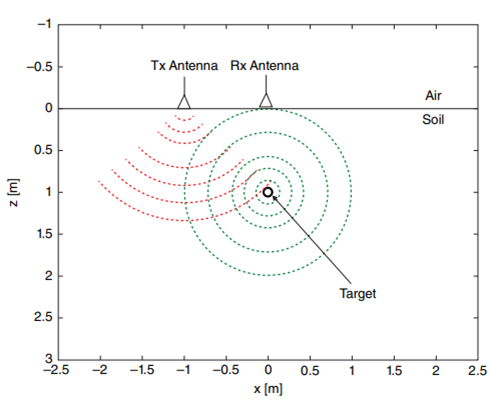
\includegraphics[scale=0.7]{gambar/bab2/gpr1.png}
  \caption{Prinsip kerja GPR \parencite{Persico2014}}
  \label{fig:GPRKerja}
\end{figure}

Ketika gelombang elektromagnetik bertemu dengan objek yang terkubur di dalam tanah, gelombang tersebar ke semua arah sesuai dengan pola tertentu. Pada penerapannya, antena pemancar dan penerima dipasang pada struktur yang kuat menjadi satu. Sinyal yang dikumpulkan biasanya ditampilkan secara real-time di layar komputer3 dan disimpan di hard disk computer. Prinsip kerja GPR tidak jauh berbeda dengan radar pada umumnya. Akan tetapi, terdapat perbedaan dalam hal teknologi, kebutuhan, aplikasi, dan pita frekuensi. GPR harus mengidentifikasi target statis, dan interpretasi data tidak diminta secara real-time. Di sisi lain, dalam prospeksi GPR gelombang elektromagnetik tidak merambat di udara tetapi malah merambat di media inang yang lebih rumit, biasanya berkerugian dan tidak homogen, mungkin dispersif, dan dalam beberapa kasus anisotropik dan/atau magnetik. GPR terbagi menjadi 2 sistem yakni pulsed dan stepped-frequency. Pulsed memancarkan dan menerima gema ke pulsa elektromagnetik. Stepped-frequency mendekomposisi pulsa elektrom agnetik menjadi komponen spektralnya dan memancarkannya secara berurutan. Akibatnya, memancarkan dan menerima kereta sinyal sinusoidal\parencite{Persico2014}.

Mengacu dari terminology data GPR untuk titik ruang disebut A-scan atau jejak GPR.
\begin{figure} [H] \centering
  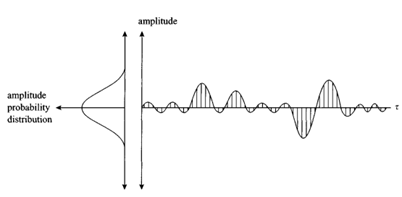
\includegraphics[scale=1]{gambar/bab2/gpr2.png}
  \caption{Sinyal A-scan \parencite{Daniels2004}}
  \label{fig:GPRAscan}
\end{figure}
Kumpulan jejak GPR untuk garis yang dipindai disebut B-scan. Meskipun GPR biasanya mengumpulkan data saat bergerak, model "stop-gather-and-go-on" dianggap cukup akurat dikarenakan perbedaan kecepatan antara sinyal elektromagnetik dan operator manusia. Penyimpanan A-scan bisa memakan waktu lebih lama karena alasan teknis.
\begin{figure} [H] \centering
  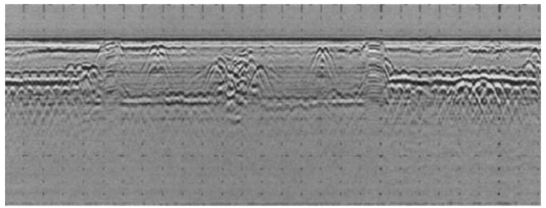
\includegraphics[scale=1]{gambar/bab2/gpr3.png}
  \caption{Sinyal B-scan \parencite{Daniels2004}}
  \label{fig:GPRBscan}
\end{figure}
Namun, menjaga kecepatan konstan saat mengumpulkan data adalah praktik terbaik. Set data GPR dari B-scan paralel disebut C-scan. Yang biasa dilihat di lapangan adalah B-scan. Data awal, atau data mentah, bisa lebih jelas setelah pemrosesan\parencite{Daniels2004}.
\begin{figure} [H] \centering
  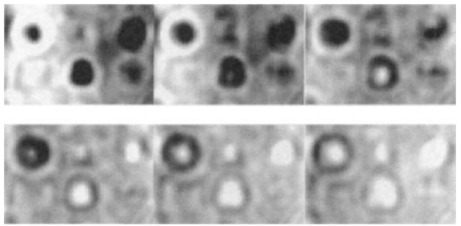
\includegraphics[scale=1]{gambar/bab2/gpr4.png}
  \caption{Sinyal C-scan \parencite{Daniels2004}}
  \label{fig:GPRCscan}
\end{figure}

\subsection{gprMax}
gprMax dikembangkan sebagai perangkat lunak lintas platform untuk Linux, Microsoft Windows, dan kemudian Mac OS X. GprMax ditulis dengan bahasa pemrograman C, dengan bagian yang memerlukan perhitungan intensif - loop solver FDTD - diparalelkan menggunakan OpenMP \parencite{Craig2016}. Pengembangan gprMax dalam implementasi fitur-fitur lanjutan baru dan untuk meletakkan dasar untuk pengembangan masa depan, diputuskan bahwa kode harus ditulis ulang menggunakan bahasa yang berorientasi objek. Python adalah bahasa yang berorientasi objek dan menampilkan pengetikan dinamis dan manajemen memori otomatis. Ini juga dimaksudkan untuk sangat mudah dibaca dan dapat diperluas. Namun, kemudahan dan fleksibilitas Python memiliki beberapa kekurangan salah satunya adalah kecepatan dalam penulisan. Kehilangan kecepatan ini dapat diatasi dengan menggunakan Cython - sebuah superset dari Python yang menghasilkan kode C yang efisien yang dapat dikompilasi menjadi modul ekstensi. Versi baru dari gprMax telah dikembangkan ulang dengan kombinasi Python, NumPy, dan Cython dengan OpenMP, yang mempertahankan manfaat Python dengan kecepatan C yang paling \parencite{Craig2015}.

gprMax menggunakan file input berupa teks di mana pengguna menentukan semua parameter untuk simulasi, misalnya, ukuran model, diskretisasi, jendela waktu, geometri, bahan, dan eksitasi. Penggunaan software gprMax sendiri tidak disertai dengan GUI. GUI tidak dikembangkan karena dinilai terlalu rumit bagi pengguna apabila berurusan dengan banyak nilai parameter yang harus diinputkan dalam satu waktu Berikut adalah contoh file input untuk simulasi GPR 2D sederhana dari silinder logam yang dikubur di setengah ruang dielektrik tanpa kerugian\parencite{Craig2016}.
\begin{figure} [H] \centering
  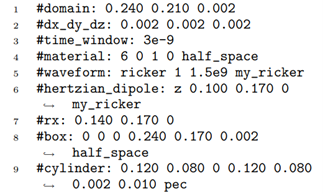
\includegraphics[scale=1]{gambar/bab2/gprmax1.png}
  \caption{Contoh file input simulasi gprMax \parencite{Craig2016}}
  \label{fig:gprMaxSim}
\end{figure}
Disamping itu, gprMax mengandung banyak fitur yang kuat dan dapat disesuaikan untuk pemodelan GPR. Selama 20 tahun terakhir, model antena telah dimasukkan dalam simulasi numerik GPR. Model antena actual telah dimasukkan terutama dari antena yang digunakan di dunia akademik atau untuk tujuan penelitian. Telah ada sedikit pekerjaan yang diterbitkan dari simulasi GPR dengan model antena komersial. Namun, kemajuan dalam kekuatan komputasi, ditambah dengan keinginan untuk menyelidiki informasi amplitudo kuantitatif dari GPR, terdapat kebutuhan untuk mengembangkan dan menggunakan model FDTD 3D rinci dari antena GPR realistis dalam simulas\parencite{Craig2016}.

GprMax2D dan GprMax3D merupakan dua program yang mengimplementasikan metode FDTD untuk pemodelan GPR di 2D dan 3D. Beberapa fiturnya adalah: antarmuka perintah yang mudah digunakan, kemampuan untuk memodelkan bahan dispersif, pemodelan target berbentuk kompleks serta simulasi ruang tak terbatas menggunakan kondisi batas penyerapan yang kuat. GprMax3D mampu mensimulasi antena GPR dan bahkan pengenalan garis transmisi pemberian mereka ke dalam model. GprMax2D digunakan untuk simulasi "signture" GPR sedangkan GprMax3D digunakan untuk simulasi yang lebih detail dan realistis terutama ketika perbandingan dengan data GPR nyata penting. Baik program GprMax2D dan 3D menggunakan file ASCII (teks) sederhana untuk mendefinisikan parameter model \parencite{Giannopoulos2005}.
\begin{figure} [H] \centering
  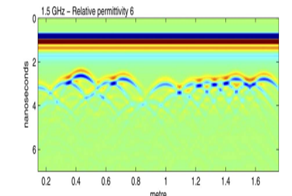
\includegraphics[scale=1]{gambar/bab2/gprmax2.png}
  \caption{Pemodelan sinyal 2D pada gprMax \parencite{Giannopoulos2005}}
  \label{fig:grMax2d}
\end{figure}
\begin{figure} [H] \centering
  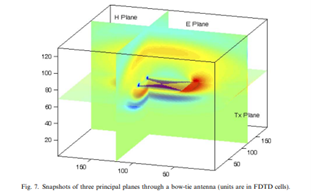
\includegraphics[scale=1]{gambar/bab2/gprmax3.png}
  \caption{Pemodelan sinyal 3D pada gprMax  \parencite{Giannopoulos2005}}
  \label{fig:grMax3d}
\end{figure}

\subsection{Python}
Python merupakan salah satu bahasa pemrograman serbaguna dan tingkat tinggi yang terkenal karena kepopularitasnya. Python berkembang pertama kali pada akhir tahun 1980-an di Belanda, oleh Guido van Rossum. Versi pertama Python yakni 0.9.0, diluncurkan pada tahun 1991, diikuti oleh Python 2.0 pada tahun 2000. Python baru berkembang secara signifikan setelah berjalan 9 tahun lagi. Periode antara tahun 2005 dan 2013 menandai era penting dalam pengembangan Python, peningkatan ini tak lepas dari upaya yang pembuat bahasa python itu sendiri. Python membedakan dirinya dengan menjadi bahasa yang diinterpretasikan, tidak memerlukan programnya untuk dikompilasi menjadi kode mesin. Sebagai gantinya, kode Python diubah menjadi bytecodes, yang kemudian dieksekusi oleh Mesin Virtual Python (PVM) yang terintegrasi dalam interpreter Python\parencite{Harris2023}.

Menekankan aksesibilitas, sintaksnya yang sederhana memudahkan pembacaan dan penggunaan. Meskipun sederhana, Python tetap menjadi bahasa serbaguna yang kuat, menawarkan pengalaman pemrograman yang lebih efisien, terutama bila dibandingkan dengan Java. Kelebihan Python terletak pada dukungannya untuk berbagai pemrograman, termasuk pemrograman terstruktur, imperatif, berorientasi objek, fungsional, dan prosedural. Akan tetapi, ia tidak mendukung pemrograman logika. python memiliki 2 kelebihan antara lain: pertama, python memiliki berbagai konstruksi dan pernyataan bahasa yang kuat untuk representasi dan manipulasi data. Kedua, python memiliki ekosistem yang luas dari paket, pustaka, dan modul pihak ketiga untuk berbagai kebutuhan pemrograman, ditambah dengan perpustakaan standar yang luas yang disertakan dalam setiap rilis Python. Keberagaman ini membuat Python menjadi pilihan populer di bidang seperti analisis data dan pembelajaran mesin, didukung oleh pustaka seperti NumPy, SciPy, Pandas, Matplotlib, dan TensorFlow\parencite{Harris2023}.

Kelebihan python bukan tanpa kekurangan, mengingat interpreter Python membentuk lapisan dasar perangkat lunak, mereka tidak terhindar dari bug perangkat lunak. Masalah dalam interpreter Python cenderung lebih luas dan berpotensi lebih merusak dibandingkan dengan bug aplikasi biasa. Penanganan dan penyelesaian dari bug-bug ini dalam interpreter Python sangat penting untuk memastikan aplikasi Python dapat berjalan seperti yang diharapkan\parencite{Ziyuan2022}.

\subsection{Convolutional Neural Network}
Artificial Neural Network (ANN) merupakan sistem pemrosesan komputasi yang terinspirasi oleh cara sistem saraf biologis otak beroperasi. ANNs terutama terdiri dari sejumlah besar node komputasi yang saling terhubung yang biasa disebut neuron dimana neuron yang bekerja bersama-sama secara terdistribusi untuk belajar secara kolektif dari input agar dapat mengoptimalkan outputnya. Convolutional Neural Network (CNN) memiliki kesamaan dengan ANN yang mana terdiri dari neuron yang mengoptimalkan diri melalui pembelajaran. Setiap neuron akan tetap menerima input dan melakukan operasi dasar dari banyak ANN. Dari vektor gambar mentah input hingga output akhir skor kelas, seluruh jaringan akan tetap mengekspresikan satu fungsi skor perseptif (bobot). Lapisan terakhir akan berisi fungsi kerugian yang terkait dengan kelas, dan semua tips dan trik reguler yang dikembangkan untuk ANNs tradisional masih berlaku\parencite{Keiron2015}.

Bisa dikatakan bahwa CNN adalah model yang cukup baik dalam bidang pemrosesan gambar. CNN dapat memberikan hasil yang baik dalam klasifikasi gambar, pengenalan, segmentasi semantik, dan terjemahan mesin, dan dapat belajar serta mengekstrak fitur gambar secara mandiri. Namun, CNN hanya bisa dioperasikan pada data reguler, seperti gambar dengan ukuran tetap\parencite{Ruyue2020}. Perbedaan yang cukup terlihat antara CNN dan ANN tradisional CNN banyak digunakan dalam bidang pengenalan pola dalam gambar. Hal ini memungkinkan pengguna dalam mengkodekan fitur khusus gambar ke dalam arsitektur, membuat jaringan lebih cocok untuk tugas yang berfokus pada gambar - sekaligus mengurangi parameter yang dibutuhkan dalam mengatur model\parencite{Keiron2015}.

CNN memiliki banyak variasi arsitektur. Namun, komponen dasar CNN bisa dikatakan mirip dimana terdiri dari tiga jenis lapisan, yaitu lapisan konvolusional, pooling, dan fully-connected. Lapisan konvolusional bertujuan untuk belajar representasi fitur dari input\parencite{Jiuxiang2018}.

\begin{figure} [H] \centering
  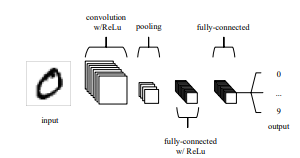
\includegraphics[scale=1]{gambar/bab2/cnn1.png}
  \caption{Arsitektur CNN sederhana \parencite{Keiron2015}}
  \label{fig:CNNArsi}
\end{figure}

Seperti pada ANN, input layer di CNN akan membawa nilai pixel dari gambar\parencite{Keiron2015}. Lapisan konvolusi terbentuk oleh beberapa kernel konvolusi yang digunakan untuk menghitung peta fitur yang berbeda. Setiap neuron dari sebuah peta fitur terhubung dengan sebuah wilayah dari neuron tetangga di lapisan sebelumnya\parencite{Jiuxiang2018}.

\begin{figure} [H] \centering
  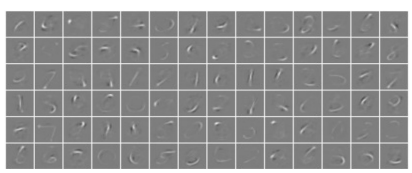
\includegraphics[scale=1]{gambar/bab2/cnn2.png}
  \caption{Aktivasi dari convolutional layer pertama \parencite{Keiron2015}}
  \label{fig:CNNConvo}
\end{figure}

Seperti namanya, lapisan konvolusi memainkan peran penting dalam cara kerja CNN. Parameter lapisan ini berfokus pada penggunaan kernel yang dapat dipelajari. Kernel ini memiliki ukuran kecil dalam dimensi spasial, tetapi menyebar sepanjang seluruh kedalaman input. Saat data mencapai lapisan konvolusi, dilakukan konvolusi setiap filter di seluruh dimensi spasial input untuk menghasilkan peta aktivasi 2D. Peta aktivasi ini dapat divisualisasikan, seperti yang terlihat pada Gambar \ref{fig:CNNConvo}. Saat melalui input, hasil kali skalar dihitung untuk setiap nilai dalam kernel. (Gambar \ref{fig:Blueprint}) Jaringan akan belajar kernel yang 'aktif' ketika mereka melihat fitur tertentu pada posisi spasial tertentu dari input. Ini umumnya dikenal sebagai aktivasi\parencite{Keiron2015}.

\begin{figure} [H] \centering
  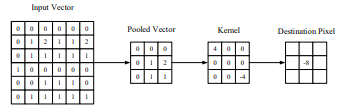
\includegraphics[scale=1]{gambar/bab2/cnn3.png}
  \caption{Representasi visual convolution layer \parencite{Keiron2015}}
  \label{fig:Blueprint}
\end{figure}

Peta aktivasi dimiliki oleh setiap layer konvolusi of yang akan ditumpuk sepanjang dimensi kedalaman membentuk volume output penuh dari lapisan konvolusi\parencite{Keiron2015}.

Lapisan pooling memiliki tujuan untuk mencapai ketidakberubahan pergeseran dengan melakukan pengurangan resolusi peta fitur. Lapisan ini berada di antara dua lapisan konvolusi. Setiap peta fitur dari lapisan pooling tersambung dengan peta fitur yang sesuai dari lapisan konvolusi sebelumnya. Setelah beberapa lapisan konvolusi dan pooling, akan terdapat lapisan fully-connected yang bertujuan untuk menalar dalam tingkat tinggi. Lapisan ini mengambil semua neuron di lapisan sebelumnya dan menghubungkannya ke setiap neuron di lapisan saat ini untuk menghasilkan informasi semantik global\parencite{Jiuxiang2018}.

Fully-connected layer berisi neuron yang terhubung langsung ke neuron di dua lapisan yang berdekatan\parencite{Keiron2015}. Lapisan terakhir dari CNNs adalah lapisan output\parencite{Jiuxiang2018}. Lapisan yang tidak kalah penting adalah lapisan ReLU. Tujuan dari ReLU adalah untuk melakukan peningkatan non-linearitas CNN. Lapisan ReLU sendiri tidak mengubah ukuran dari input dan lapisan ini tidak memiliki parameter. Pada penerapannya, lapisan ini aman untuk digunakan karena lapisan ReLU akan mengatur semua nilai negatif menjadi nol\parencite{Wu2017}.

\subsection{Roboflow}
Roboflow adalah situs web yang memiliki banyak koleksi terhadap berbagai jenis dataset. Website ini juga menyediakan data dalam berbagai pilihan format untuk berbagai model machine learning\parencite{Deepa2023}. Setidaknya, Roboflow memiliki lebih dari 100.000 pengguna yang telah mengumpulkan dan melabeli dataset mereka sendiri untuk kebutuhan kustom mereka. Hal tersebut menyebabkan Roboflow Universe telah banyak digunakan oleh para peneliti untuk digunakan dalam berbagai projek mereka khususnya dalam proyek deteksi objek\parencite{ciaglia2022}.


Sebagai platform computer vision, Roboflow digunakan untuk melatih model karena kemudahan dan kecepatan yang dimiliki dalam membuat model tanpa harus melalui proses pemrograman yang intensif. Roboflow memiliki fitur untuk mempersiapkan data, melatih dan mengembangkan model, serta banyak hal lainnya yang membuatnya menjadikan Roboflow sebagai platform dengan infrastruktur untuk mempercepat proses pembuatan model computer vision. RoboFlow menawarkan rangkaian lengkap alat dan layanan dengan tujuan menyederhanakan dan mempercepat pengembangan dan penerapan model computer vision. Hal ini sangat berguna dalam penggunaan visi komputer pada aplikasi dan proyekb bagi pemrogram dan perusahaan. Fitur dan kemampuan utama RoboFlow meliputi anotasi data dan persiapan untuk memberi label pada video dan gambar, yang keduanya diperlukan untuk mengajarkan model computer vision untuk mengidentifikasi dan menemukan lokasi objek dalam gambar. Dengan menghasilkan varian data asli, RoboFlow menawarkan berbagai strategi augmentasi data yang membantu model machine learning menjadi lebih baik. Model computer vision tersebut nantinya dapat dilatih menggunakan TensorFlow, PyTorch, dan YOLO\parencite{Brucal2023}.

\subsection{YOLO}
You Only Look Once (YOLO) adalah algoritma yang populer dan banyak digunakan. YOLO terkenal dengan karakteristik pendeteksi objeknya. YOLO pertamakali diperkenalkan pada tahun 2015. Dalam beberapa tahun terakhir, YOLO telah mengalami perkembangan dan mencapai versi yang lebih baru seperti YOLO V2, YOLO V3, YOLO V4, YOLO V5, dan seterusnya hingga YOLO V9. Ada beberapa versi revisi terbatas, seperti YOLO-LITE. Ukuran model yang kecil dan kecepatan perhitungan yang cepat merupakan inti dari algoritma deteksi target YOLO. YOLO cepat karena YOLO hanya perlu memasukkan gambar ke dalam jaringan untuk mendapatkan hasil deteksi akhir, sehingga YOLO juga dapat mengukur waktu deteksi video. YOLO secara langsung menggunakan gambar global untuk deteksi, yang dapat mengkodekan informasi global dan mengurangi kesalahan dalam mendeteksi latar belakang sebagai objek. Hasil tes YOLO tidak bagus untuk objek yang jaraknya sangat dekat satu sama lain dan dalam kelompok. Kinerja yang buruk ini disebabkan karena hanya dua kotak dalam grid yang diprediksi dan hanya termasuk dalam kelas objek baru dari kategori yang sama, sehingga muncul rasio aspek yang tidak normal, dan kondisi lain, seperti kemampuan generalisasi yang lemah\parencite{Jiang2022}.

Arsitektur YOLO asli terdiri dari 24 convolution layers, diikuti oleh dua lfully connected layers. YOLO memprediksi lebih dari satu kotak pembatas per sel kisi dimana kotak pembatas yang memiliki Intersection Over Union (IOU) tertinggi dengan ground truth dipilih, yang dikenal sebagai non-maxima suppression. YOLO memiliki dua cacat yaitu satu adalah posisi yang tidak akurat, dan yang lainnya adalah tingkat recall yang lebih rendah dibandingkan dengan metode berdasarkan rekomendasi area\parencite{Jiang2022}. YOLO bukanlah algoritma pertama yang menggunakan Single Shot Detector (SSD) untuk mendeteksi objek. Single Shot Detector (SSD), Deconvolution Single Shot Detector (DSSD), RetinaNet, M2Det, dan RefineDet++ merupakan algoritma yang telah ada sebelum YOLO untuk melakukan pendeteksian objek secara satu tahap. YOLO kelebihan sebagai pendeteksi objek dua tahap dalam hal akurasi dan waktu inferensi. Selain itu, dengan munculnya YOLO, berbagai aplikasi telah menggunakan YOLO untuk mendeteksi dan mengenali objek dalam berbagai konteks dan memiliki performa yang sangat baik dibandingkan dengan pendeteksi objek dua tahap lainnya\parencite{Diwan2022}.

\subsection{Google Colab}
Google Colab adalah environment Jupyter notebook yang berjalan di Google cloud. Colab memungkinkan pengguna lain untuk menggunakan dan berbagi notebook Jupyter tanpa harus mengunduh, menginstal, atau menjalankan apa pun. Jupyter sendiri merupakan adalah proyek open source yang bekerja pada browser yang menyematkan bahasa skrip, pustaka, dan alat untuk visualisasi. Setiap file buku catatan di Jupyter terdiri dari beberapa sel, di mana memiliki outputnya menyatu dalam dokumen termasuk teks, tabel, bagan, dan grafik. Google Colab menyediakan akses langsung ke Google Drive dan GitHub serta layanan cloud gratis dengan GPU dan TPU. Platform perangkat keras yang banyak tersedia di cloud adalah CPU, TPU, dan GPU. CPU gratis untuk Google Colab dilengkapi dengan 2-core Intel Xeon @2.0GHz dan RAM 13 GB serta HDD 33 GB. Masa pakai maksimum VM di Google Colab adalah 12 jam dengan waktu idle 90 menit\parencite{Kimn2021}.

\begin{figure} [H] \centering
  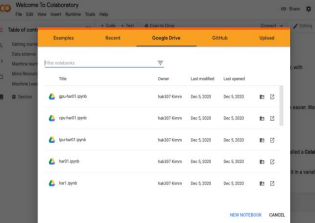
\includegraphics[scale=1]{gambar/bab2/colab.png}
  \caption{Google Colab \parencite{Kimn2021}}
  \label{fig:colab}
\end{figure}

Google Colaboratory adalah platform dapat digunakan untuk melakukan edukasi dan penelitian mengenai machine learning. Colaboratory menyediakan runtime Python 2 dan 3 yang telah dikonfigurasi sebelumnya dengan pustaka machine learning dan AI yang penting, seperti TensorFlow, Matplotlib, dan Keras. Google Colaboratory dapat digunakan secara efektif untuk mempercepat tidak hanya deep learning tetapi juga aplikasi ilmiah berbasis GPU lainnya\parencite{Carneiro2018}.

\subsection{Tensorflow}
Dibuat oleh peneliti yang berasal dari Google, TensorFlow adalah pustaka yang paling populer di antara kebanyakan pustaka lainnya. TensorFlow adalah pustaka perangkat lunak yang fleksibel dan skalabel untuk komputasi numerik menggunakan grafik dataflow. Dengan menggunakan pustaka TensorFlow ini, pengguna mampu memprogram dan melatih neural network serta model machine learning lainnya secara efisien dan menerapkannya ke produksi. Algoritme inti TensorFlow ditulis dalam C++ dan CUDA (Compute Unified Device Architecture) secara optimal. CUDA sendiri merupakan sebuah platform komputasi paralel dan API yang dibuat oleh NVIDIA. CUDA memiliki API yang tersedia dalam beberapa bahasa. Bahasa yang didukung secara resmi oleh TensorFlow adalah JavaScript, C++, Java, Go, dan Swift. TensorFlow juga tersedia untuk lebih banyak bahasa seperti C\# dan Ruby. Akan tetapi, API untuk bahasa pemrograman Python adalah yang paling lengkap dan stabil\parencite{Pang2019}.

TensorFlow adalah platform machine learning menyeluruh yang didukung oleh Google. Pada dasarnya, program TensorFlow terdiri dari dua bagian utama: bagian konstruksi, yang memungkinkan pembuatan model jaringan machine learning atau deep learning, dan bagian eksekusi, yang memungkinkan untuk melatih dan mengevaluasi model jaringan. TensorFlow menyediakan API yang paling banyak digunakan karena kelengkapan dan stabilitasnya yang disajikan dalam bahasa pemrograman Python untuk mencapai kedua bagian tersebut. TensorFlow juga menyediakan pustaka TensorFlow Lite untuk penerapan model jaringan pada perangkat seluler, mikrokontroler, dan perangkat edge. TensorFlow Lite memungkinkan konversi model TensorFlow dasar menjadi versi terkompresi melalui apa yang disebut konverter TensorFlow Lite. Tensorflow sendiri memiliki Keras yang mana merupakan sebuah kerangka deep learning. Keras dibangun di atas TensorFlow versi 2, yang menyediakan API Python untuk memungkinkan pengembang menyederhanakan pembuatan dan eksperimen model jaringan\parencite{Contoli2023}.

\subsection{PyCUDA}
PyCUDA merupakan sebuah API (Application Programming Interface) dari bahasa pemrograman python untuk mengakses kartu grafis NVIDIA menggunakan CUDA. PyCUDA Banyak digunakan sebagai API untuk bahasa pemrograman python adalah karena kode yang ditulis seperti kode python biasa dan penanganan kesalahan juga lebih sederhana daripada bahasa C atau CUDA itu sendiri\parencite{Koprawi2020}. PyCUDA merepresentasikan pendekatan berbasis skrip untuk generasi kode runtime GPU. PyCUDA memberikan kemudahan akses untuk bahasa pemrograman python. Salah satu kemudahan itu ditunjukkan dengan memberikan pengguna akses ke API komputasi paralel milil NVIDIA itu sendiri. Hal tersebut memungkinkan kode CUDA untuk disematkan sebagai string dalam skrip bahasa pemrograman python. String tersebut akan diuraikan oleh pycuda.compilerSourceModule, yang mana akan dikompilasi menggunakan nvcc sebagai driver kompilator CUDA dan terhubung dengan library runtime CUDA. PyCUDA memungkinkan pengguna untuk mengakses GPU NVIDIA menggunakan CUDA dari bahasa pemrograman Python. PyCUDA dirancang untuk pengembang CUDA yang ingin mengintegrasikan kode yang sudah ditulis dalam CUDA dengan Python\parencite{leung2023experience}.

\subsection{NextJS}
Next.JS adalah framework tangguh yang mampu meningkatkan kinerja situs web dan SEO melalui berbagai teknik pengoptimalan. Next.js juga menerapkan Incremental Static Regeneration (ISR) dan mengurangi ukuran beban JavaScript melalui pemisahan kode dan React. Selain kemampuan pengoptimalan dan peningkatan kinerjanya, Next.JS juga menawarkan serangkaian fitur yang memudahkan pengembang dalam membangun dan memelihara situs web mereka. Next.js menyediakan fitur hot reload yang memungkinkan pengembang membuat perubahan pada kode mereka dan melihat hasilnya secara real time tanpa memuat ulang halaman secara manual. Ini bisa menjadi penghemat waktu yang sangat besar bagi pengembang, memungkinkan mereka menguji dan mengulangi kode mereka dengan cepat tanpa perlu pemuatan ulang yang berulang\parencite{Patel2023}. Sebagai salah satu framework yang sering terkenal dan sering digunakan untuk mengembangkan website, Next.js memiliki beberapa kelebihan dalam pengaplikasiannya. Kelebeihan pertama yang dimiliki oleh Next.js adalah didukung dengan kemampuan untuk menggunakan CSS secara langsung pada Next.js. Berbeda dengan penggunaan CSS pada umumnya dimana modul CSS berisi pengaturan CSS untuk semua komponen, pada Next.js terdapat Global CSS yang memungkinkan kode CSS dapat diakses oleh semua komponen\parencite{lazuardy2022}.

\begin{figure} [H] \centering
  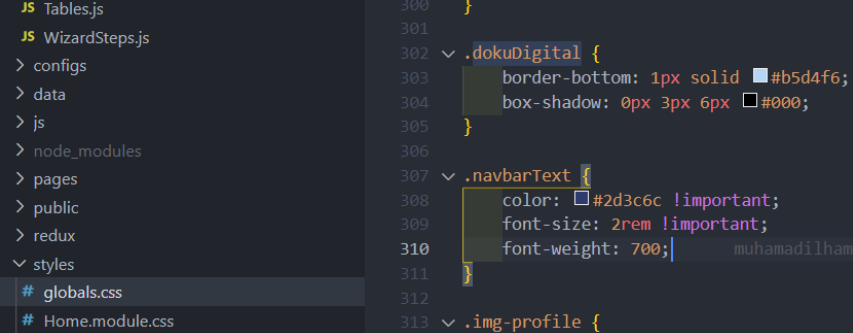
\includegraphics[scale=0.5]{gambar/bab2/builtincss.png}
  \caption{Built-in CSS pada Next.js \parencite{lazuardy2022}}
  \label{fig:builtincss}
\end{figure}

Kelebihan selanjutnya adalah framework Next.js sudah memiliki dukungan mekanisme routing terletak pada folder pages, sehingga tidak memerlukan pustaka tambahan untuk melakukan routing. Routing komponen React cukup dengan menuliskan nama file langsung di folder pages yang disediakan oleh Next.js. Dengan ini, pengguna mampu memasukkan komponen-komponen yang terdapat pada folder komponen ke dalam file routing yang telah disatukan dengan Layout komponen sebagai komponen statis sehingga suatu komponen dapat ditampilkan selama proses pengunggahan\parencite{lazuardy2022}.

\begin{figure} [H] \centering
  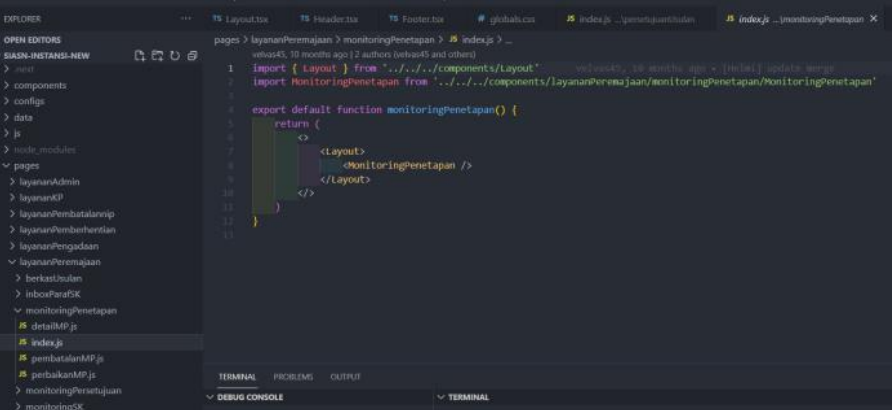
\includegraphics[scale=0.5]{gambar/bab2/routing.png}
  \caption{Routing pada Next.js\parencite{lazuardy2022}}
  \label{fig:routingnextjs}
\end{figure}

Selain itu, kelebihan lain yang dimiliki oleh Next.js adalah Framework Next.js sudah mendukung SSR dalam merender halaman web, sehingga membuat pengguna tidak akan melihat halaman kosong pada pemuatan awal dan mengurangi beban pada browser \parencite{lazuardy2022}.

\begin{figure} [H] \centering
  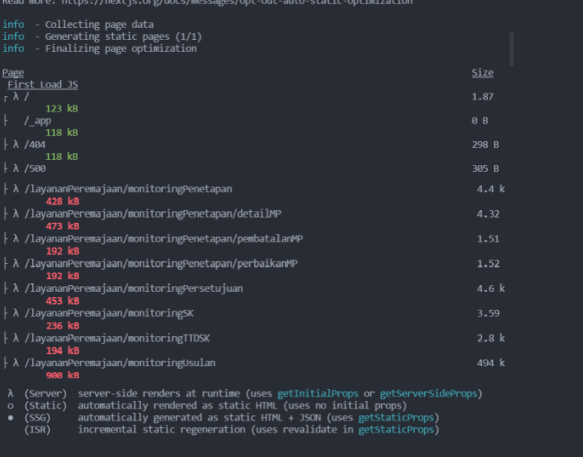
\includegraphics[scale=1]{gambar/bab2/prerender.png}
  \caption{Pre-rendering pada Next.js \parencite{lazuardy2022}}
  \label{fig:prerenderingnextjs}
\end{figure}

Framework Next.js mendukung mekanisme pengambilan data dengan CSR, SSR, SSG, dan ISR yang mana tidak seperti aplikasi React.js biasa yang hanya mendukung pengambilan data dengan CSR. Sehingga mekanisme pengambilan data dapat disesuaikan dengan kebutuhan aplikasi. Menggunakan SSR (server-side rendering) lebih baik untuk SEO (searchengine optimization), daripada CSR (client-side rendering) karena file HTML dirender di sisi server\parencite{lazuardy2022}. Terlepas dari kelebihan ang disebutkan di atas Next.JS mampu melakukan hosting situs web dengan mudah, dengan opsi untuk hosting di platform seperti Vercel dan GitHub Pages. Opsi hosting ini memberi pengembang cara yang nyaman sehingga lebih mudah untuk fokus dalam membangun dan mengoptimalkan situs\parencite{Patel2023}.

\subsection{FastAPI}
FastAPI adalah framework Python berbasis web yang menyediakan lapisan bagi model ML untuk memberikan kinerja tinggi dan mengekspos fungsionalitas model ML sebagai layanan mikro yang tenang. FastAPI terintegrasi dengan baik ke dalam tampilan yang lebih sederhana untuk memprediksi hasil model ML. Aplikasi ini dapat dengan mudah diakses melalui  web browser di Internet. Waktu respon aplikasi FastAPI cukup singkat dibandingkan aplikasi berbasis Flask. Selain itu, biometrik perilaku berpotensi meningkatkan keamanan akun pengguna dan mengurangi jumlah ancaman dan kerentanan tanpa memerlukan perangkat keras tambahan. Studi ini memberikan gambaran komprehensif mengenai penelitian atau upaya yang dilakukan untuk mengintegrasikan model ML dengan FastAPI untuk biometrik perilaku guna memberikan solusi yang lebih cepat dan hemat biaya dibandingkan Flask. Proses pengembangan lebih cepat berkat otomatisasi canggih editor dan pemeriksaan kesalahan otomatis yang disediakan oleh framework \parencite{Bansal2022}.

\subsection{Redis}
Redis adalah penyimpanan struktur data in-memory open-source yang dapat digunakan sebagai database, cache, dan perantara pesan. Redis mendukung berbagai struktur data, termasuk string, hashes, lists, sets, dan sorted sets. Dikenal karena kinerjanya yang luar biasa, Redis dapat menyimpan seluruh kumpulan data di memori, yang secara signifikan mempercepat akses data dibandingkan dengan database berbasis disk. Redis++ memperbaiki manajemen memori dan pengindeksan, yang meningkatkan kinerja dan mengurangi masalah fragmentasi memori dan kehilangan cache\parencite{Zhang2018}. Redis telah diadaptasi untuk menggunakan teknologi RDMA melalui InfiniBand untuk lebih mempercepat kinerja dengan mengurangi latensi jaringan dan pemanfaatan CPU\parencite{Tang2017}. Selain itu, Redis telah diperluas untuk menyertakan fitur keamanan seperti autentikasi dan enkripsi, sehingga lebih cocok untuk aplikasi perusahaan yang memerlukan penanganan data yang aman\parencite{Zaki2015}.

\subsection{Typescript}
Salah satu bahasa pemrograman yang sedang populer untuk mengembangkan aplikasi web adalah TypeScript \parencite{Thu2021}.  TypeScript berkembang sebagai alternatif dari JavaScript yang menerapkan pengecekan tipe statis. Telah banyak perkembangan dan penambahan fitur serta sintax baru dalam bahasa ini. Namun, TypeScript tidak memiliki spesifikasi formal \parencite{Scarsbrook2023}. Perkembangan dari TypeScript diikuti dengan banyaknya pengguna yang menggunakan bahasa ini sebagai bahasa untuk mengembangkan aplikasi website. Akan tetapi, tidak semua fitur yang ada di TypeScript diadopsi oleh pengguna. Pengadopsian TypeScript ini juga mempunyai tantangan \parencite{Thu2021} Beberapa fitur bahasa baru jarang diadopsi oleh proyek-proyek yang ada. Hal ini dikarenakan adopsi fitur baru dalam bahasa TypeScript membutuhkan waktu yang cukup lama. Sebuah proyek dapat memperbarui versi TypeScript tanpa mengubah kode mereka sama sekali, sehingga tanpa mengadopsi fitur baru. Sehingga, mengadopsi fitur baru mungkin memerlukan adopsi versi TypeScript yang baru, tetapi tidak sebaliknya. Hal ini bisa dilihat dari jumlah repositori yang mengadopsi TypeScript terbaru yang berjumlah kurang lebih 1/3 dari mayoritas repositori setelah adanya versi baru dari TypeScript itu sendiri \parencite{Scarsbrook2023}.

\cleardoublepage

% Bab 3 desain dan implementasi
\chapter{METODOLOGI}
\label{chap:metodologi}

% Ubah bagian-bagian berikut dengan isi dari desain dan implementasi

Penelitian ini dilaksanakan sesuai dengan desain sistem berikut ini beserta implementasinya. Desain sistem merupakan konsep dari pembuatan dan perencangan infrastruktur dan kemudian diwujudkan dalam bentuk blok-blok alur yang harus dikerjakan.

\section{Deskripsi Sistem}
\label{sec:deskripsisistem}

Tugas akhir ini merupakan penelitian yang menggunakan teknologi deep learning agar dapat mendeteksi keberadaan rongga udara di dalam beton. Secara umum penelitian kali ini akan menggunakan desain sistem sesuai dengan Gambar \ref{fig:metodologi}.

\begin{figure} [H] \centering
  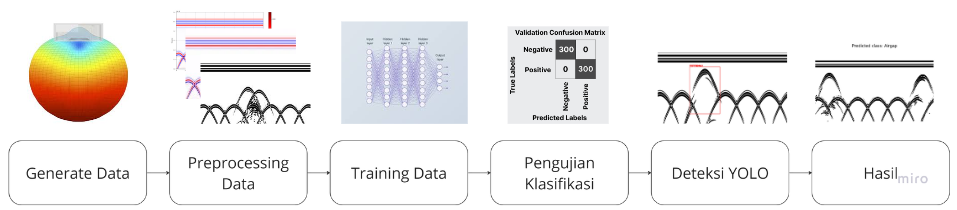
\includegraphics[scale=0.1]{gambar/bab3/flow.png}
  \caption{Blok Diagram Penelitian}
  \label{fig:metodologi}
\end{figure}

\subsection{\emph{Generate} Data}
Data sinyal GPR yang didapatkan merupakan data hasil simulasi menggunakan software gprMax. Setiap sinyal yang dihasilkan berbentuk B-Scan 2 dimensi. Pada penelitian kali ini, dihasilkan berjumlah 4000 data sinyal dengan 2000 data sinyal untuk beton berisi rongga udara dan rebar dan 2000 data sinyal untuk beton berisi rebar. 2000 File input untuk generate data sinyal berisi rongga udara dihasilkan menggunakan kode python untuk mempersingkat waktu pembuatan file input generate data. Kode python tersebut menghasilkan file input yang menghasilkan data sinyal untuk rongga udara secara acak sesuai dengan ketentuan yang telah dijabarkan pada BAB I. Data sinyal gprMax yang berisi rongga udara akan digenerate dengan menggunakan GPU secara online pada platform vast.ai karena keterbatasan hardware yang dimiliki oleh penulis. Berikut ini adalah spesifikasi dari GPU yang digunakan sebagai mana pada tabel \ref{tab:gpu}.

\begin{table}[H]
  \centering
  \begin{tabular}{|>{\bfseries}l|l|}
    \hline
    \textbf{Brand}         & NVIDIA       \\ \hline
    \textbf{Type}          & RTX 3060     \\ \hline
    \textbf{Number of GPU} & 1            \\ \hline
    \textbf{Disk Space}    & 20           \\ \hline
    \textbf{OS}            & Ubuntu 20.04 \\ \hline
    \textbf{API}           & CUDA         \\ \hline
  \end{tabular}
  \caption{spesifikasi GPU}
  \label{tab:gpu}
\end{table}

untuk data sinyal beton dengan rebar tanpa rongga udara, dihasilkan dengan cara yang sedikit berbeda. Pada awalnya, data ini digenerate dengan cara yang sama dengan data berisi rongga udara, akan tetapi setelah beberapa data, gambar sinyal yang dihasilkan memiliki banyak kemiripan. Sehingga data ini digenerate dengan cara lain. Pertama digenerate dua gambar sinyal yakni sinyal beton dengan rebar terstruktur dan gambar sinyal beton dengan rebar yang memiliki sedikit perubahan posisi, tepatnya satu rebar memiliki jarak antar rebar 10 cm. Dua gambar tersebut disatukan secara menyamping dan diproses menggunakan python untuk merubah posisi sinyal pada frame satu gambar dari dua gambar yang telah disatukan dengan perpindahan posisi sinyal secara horizontal dan vertikal per beberapa pixel. 

\subsection{\emph{Preprocessing} Data}
Sinyal gprMax yang memiliki rongga udara dalam bentuk .out yang telah digenerate, akan dilakukan proses untuk menghilangkan atribut bawaan gambar dari gprMax sehingga gambar hanya akan menampilkan gambar sinyal dan memotong ukuran gambar tersebut. Untuk gambar sinyal yang tidak memilki rongga udara, gambar tersebut akan di format ulang agar dapat diproses karena memilki format gambar yang berbeda dengan gambar hasil \emph{generaate} gprMax. Data simulasi sinyal B-Scan gprMax yang telah dipotong akan dilakukan proses binarization yang akan membuat gambar menjadi berwarna hitam putih untuk mengurangi ukuran file dari data tersebut dan model hasil training. Berikut ini adalah gambar sinyal sebelum dan sesudah diproses seperti yang dapat dilihat pada Gambar \ref{fig:beforeclean}, gambar \ref{fig:afterclean}, dan gambar \ref{fig:binary}

Berikut ini adalah contoh hasil generate data sinyal gprMax yang dapat dilihat pada Gambar \ref{fig:beforeclean} dan \ref{fig:afterclean}.

\begin{minipage}{\linewidth}
  \begin{figure} [H] \centering
    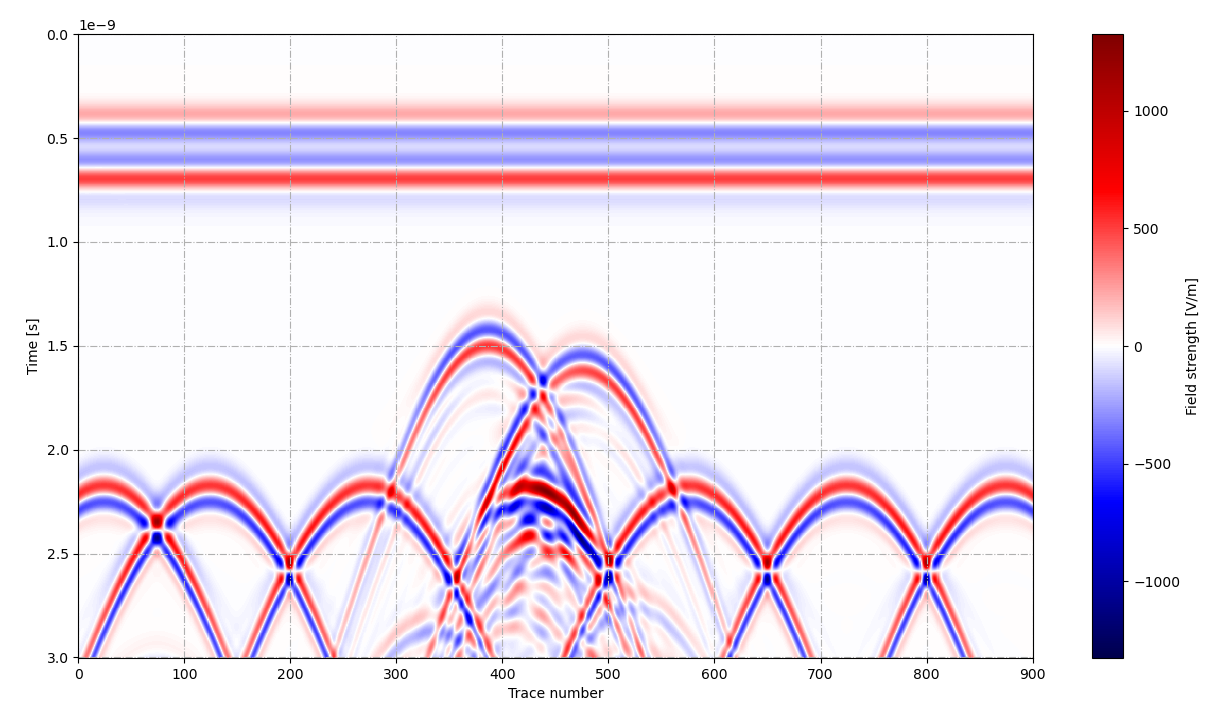
\includegraphics[scale=0.5]{gambar/bab3/beforeclean.png}
    \caption{Data Sinyal gprMax Setelah Dibersihkan}
    \label{fig:beforeclean}
  \end{figure}
\end{minipage}

\begin{minipage}{\linewidth}
  \begin{figure} [H] \centering
    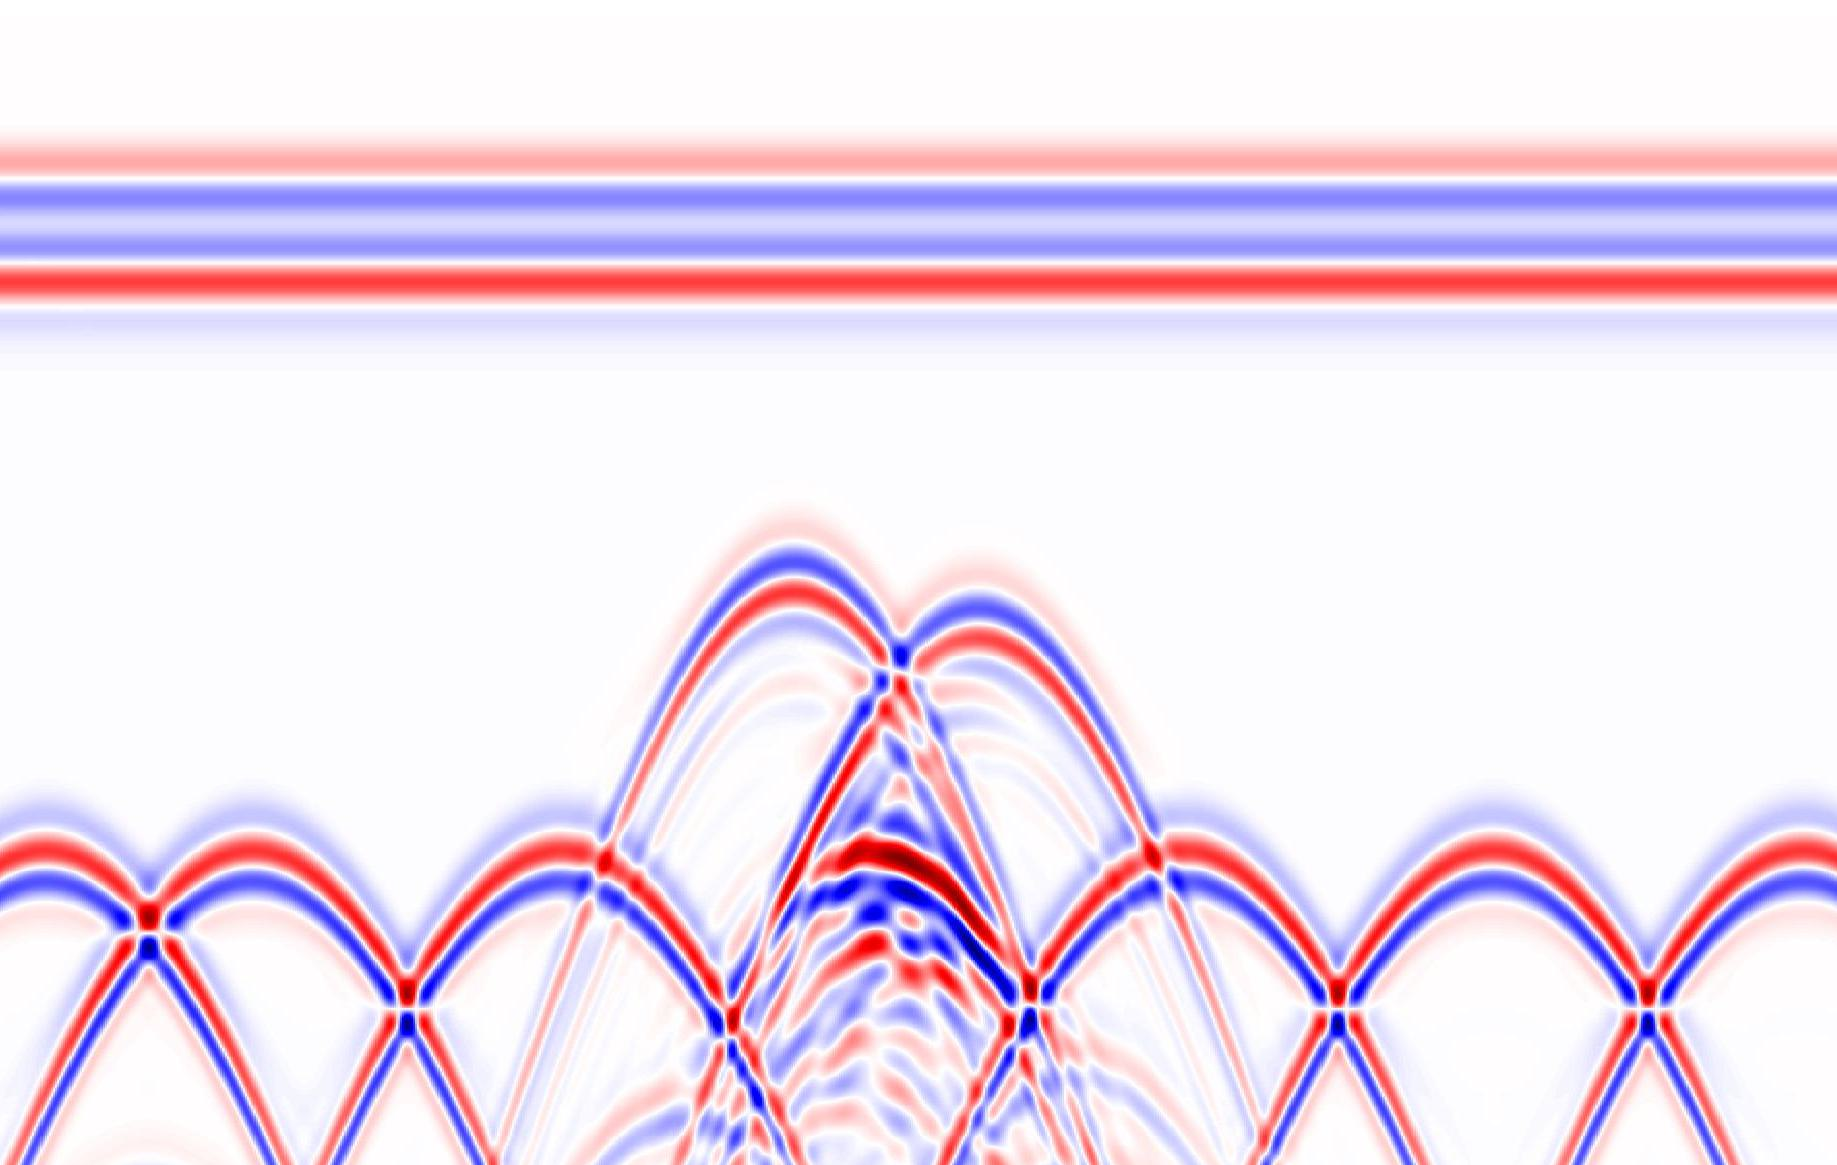
\includegraphics[scale=0.1]{gambar/bab3/afterclean.jpg}
    \caption{Data Sinyal gprMax Setelah Dibersihkan}
    \label{fig:afterclean}
  \end{figure}
\end{minipage}

\begin{figure} [H] \centering
  
\includegraphics[scale=0.1]{gambar/bab3/binary.jpg}
  \caption{Data Sinyal gprMax Setelah Dibersihkan}
  \label{fig:binary}
\end{figure}

\subsection{\emph{Training} Data}
Dataset yang telah dihasilkan terbagi menjadi dua kelas yakni 'airgap' dan 'noarigap'. Data tersebut akan dilakukan proses training untuk klasifikasi. Terdapat dua metode klasifikasi yang digunakan yakni CNN 2-Dimensi dan Roboflow. Pada CNN 2D, diterapkan berbagai macam pembagian dataset untuk training, validasi, dan testing. Pembagian dataset yang akan diujikan untuk training, validasi, dan testing antara lain 70/20/10, 70/15/15, dan 60/20/20. Model CNN 2D yang akan digunakan untuk pembagian dataset dapat dilihat pada tabel \ref{fig:cnnarc1}.

  \begin{figure} [H] \centering
    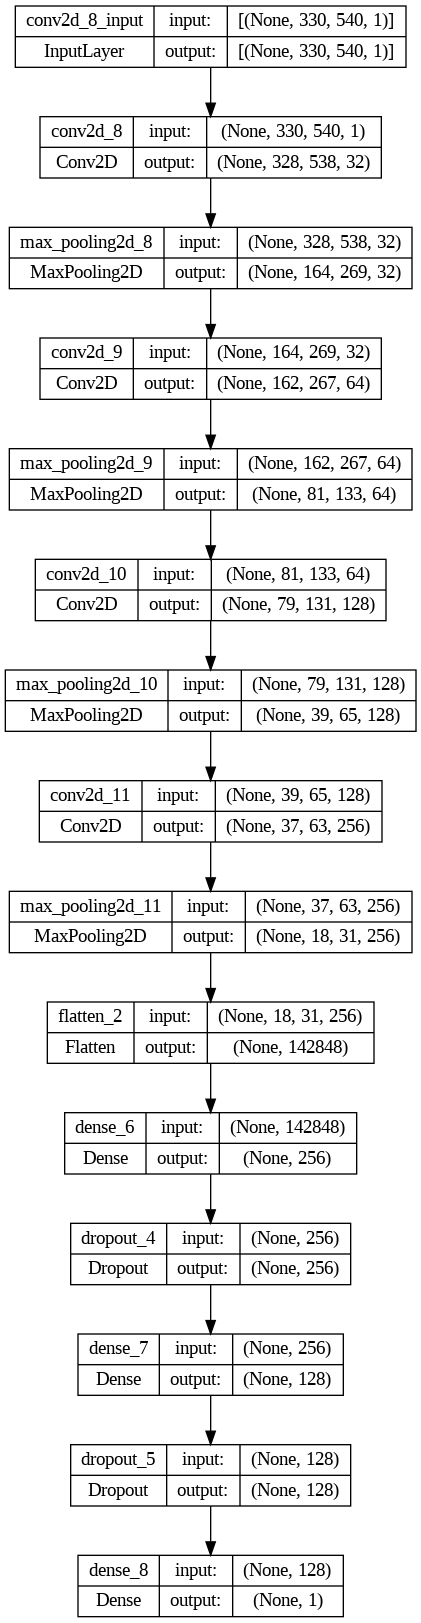
\includegraphics[scale=0.4]{gambar/bab3/cnnarc1.png}
    \caption{Arsitektur Model CNN 2D Pertama}
    \label{fig:cnnarc1}
  \end{figure}

Setelah didapatkan hasil pembagian data yang baik, pembagian data tersebut nantinya akan diterapkan pada struktur CNN 2-Dimensi yang divariasi untuk menemukan bagaimana struktur CNN 2-Dimensi yang optimal pada percobaan keempat, kelima, keenam dan ketujuh. Variasi model CNN 2D yang akan digunakan dapat dilihat pada tabel \ref{fig:cnnarc2}, tabel \ref{fig:cnnarc3}, tabel \ref{fig:cnnarc4}, dan tabel \ref{fig:cnnarc5}. CNN 2-Dimensi yang digunakan pada percobaan ini didapatkan dengan bantuan ChatGPT. Sementara itu, untuk model CNN 2D yang digunakan pada percobaan ketujuh, diambil dari peneltian yang berjudul \emph{"Classification of soil types from GPR B Scans using deep learning techniques"} \parencite{Barkataki2021}.

  \begin{figure} [H] \centering
    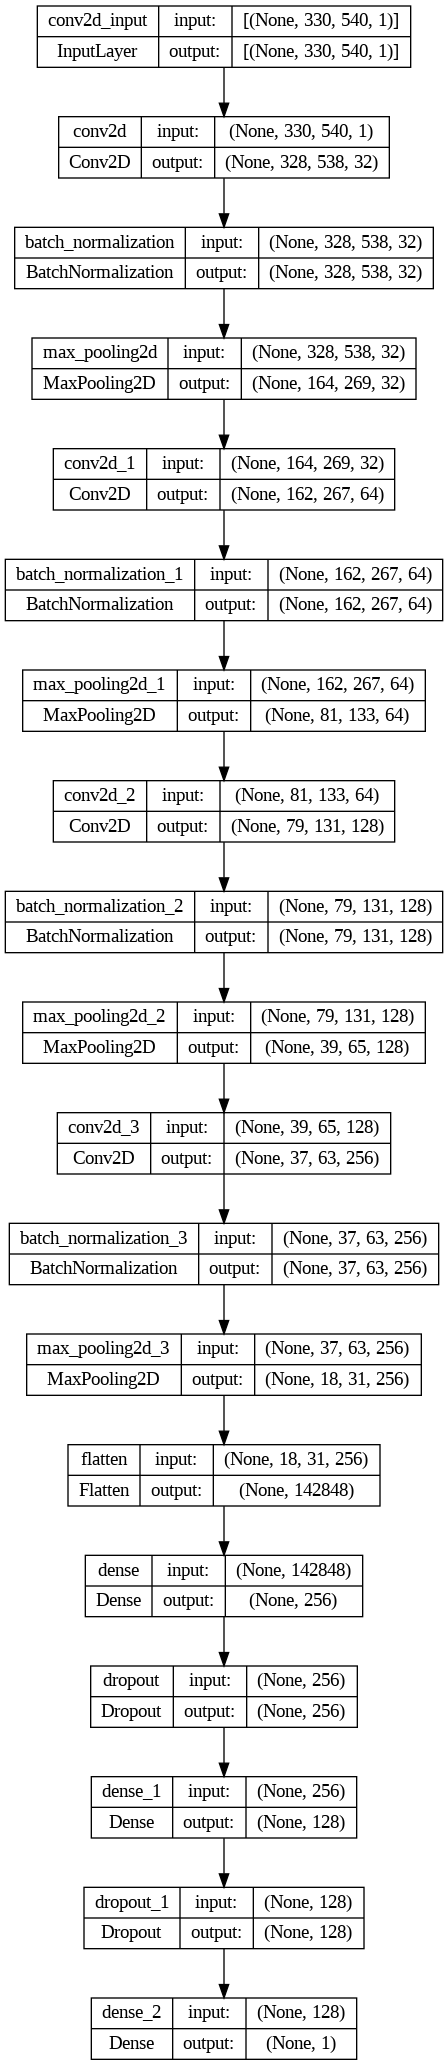
\includegraphics[scale=0.3]{gambar/bab3/cnnarc2.png}
    \caption{Arsitektur Model CNN 2D Kedua}
    \label{fig:cnnarc2}
  \end{figure}

  \begin{figure} [H] \centering
    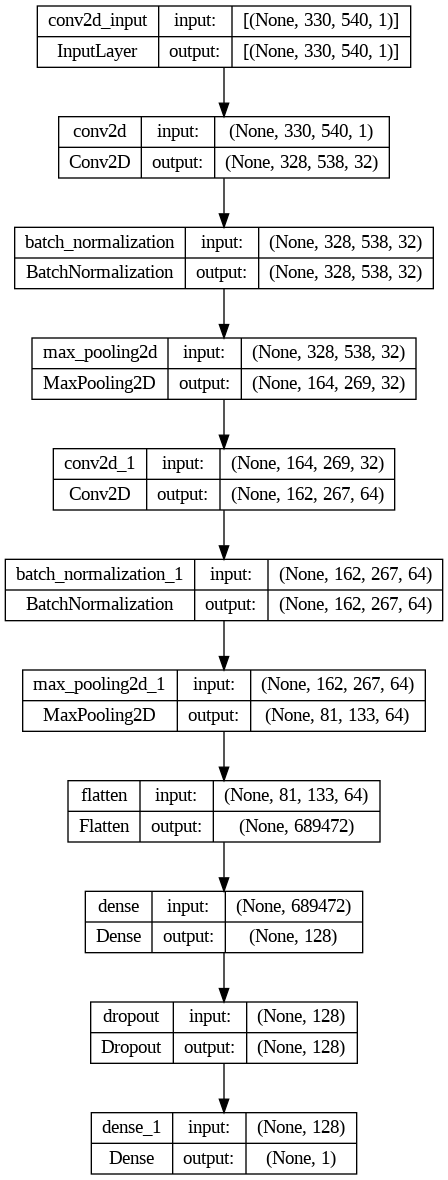
\includegraphics[scale=0.4]{gambar/bab3/cnnarc3.png}
    \caption{Arsitektur Model CNN 2D Ketiga}
    \label{fig:cnnarc3}
  \end{figure}

  \begin{figure} [H] \centering
    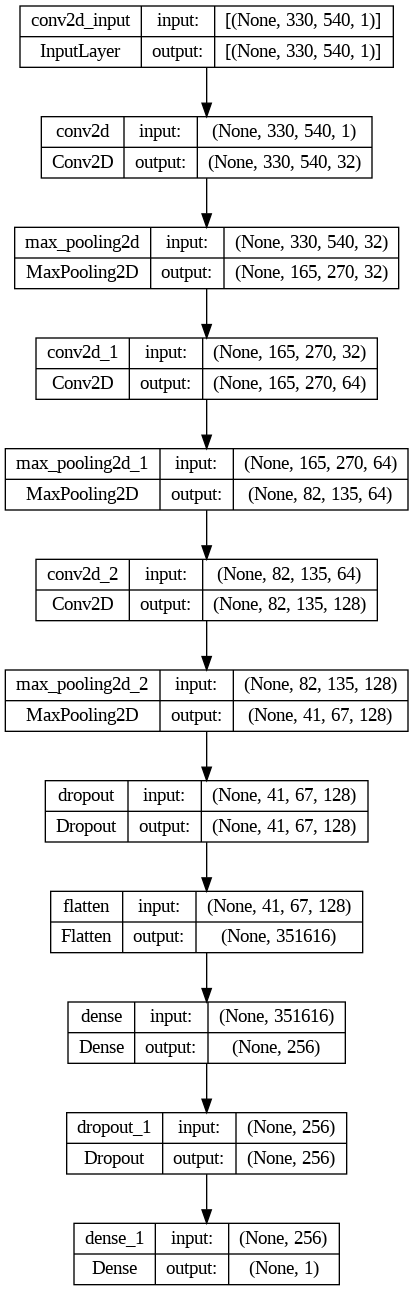
\includegraphics[scale=0.4]{gambar/bab3/cnnarc4.png}
    \caption{Arsitektur Model CNN 2D Keempat}
    \label{fig:cnnarc4}
  \end{figure}

  \begin{figure} [H] \centering
    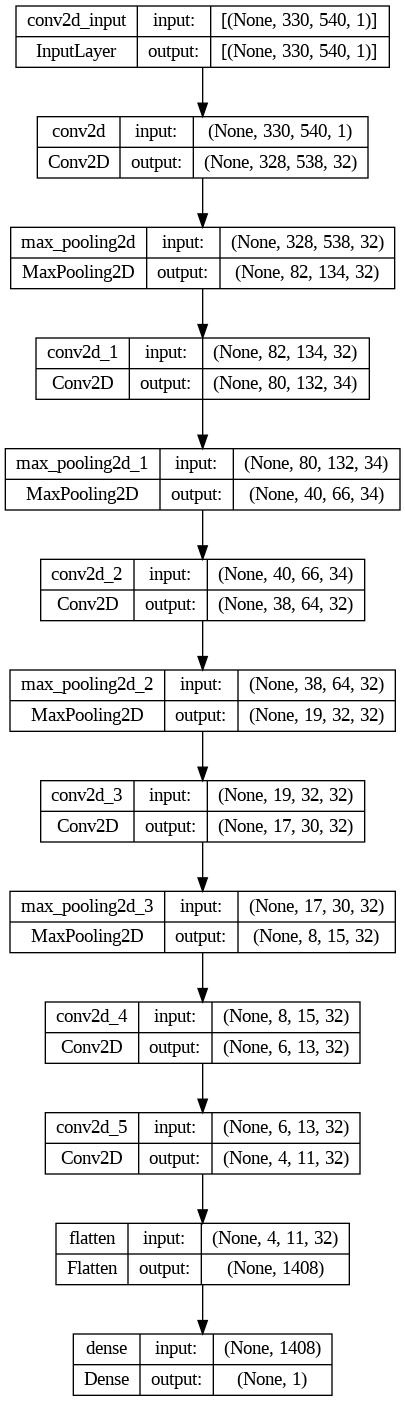
\includegraphics[scale=0.4]{gambar/bab3/cnnarc5.png}
    \caption{Arsitektur Model CNN 2D Kelima}
    \label{fig:cnnarc5}
  \end{figure}

Sementara pada Roboflow, proses klasifikasi cukup hanya dengan menetapkan gambar pada salah satu kelas. Kemudian dilakukan proses augmentasi pada data tersebut antara lain: flip (horizontal and vertical), rotate (90 degrees clockwise and counter-clockwise), crop (20\% maximum zoom), noise (up to 0.93\% pixels), dan blur (up to 1 px). Pada Roboflow, pembagian kelas awal adalah 70/20/10 untuk training, validation, dan testing. Persentase tersebut berubah setelah ditambahkan proses augmentasi menjadi 88/8/4.

\subsection{Pengujian Klasifikasi}
Pengujian klasifikasi dilakukan dengan melakukan test pada data validasi yang kemudian hasilnya akan membentuk confussion matrix. Pengujian klasifikasi juga akan dilakukan terhadap data yang dipersiapkan untuk testing diawal proses training. Pada platform, roboflow, pengujian klasifikasi cukup dilakukan dengan menguggah gambar yang hendak diuji, berikutnya platfor Roboflow akan otomatis mengklasifikasikan gambar kelas tersebut.

\subsection{Deteki YOLOv9}
YOLO yang digunakan pada training kali ini adalah YOLOv9. Versi ini dipilih karena YOLOv9 masih tergolong baru sehingga belum banyak digunakan oleh banyak orang. Model YOLOv9 ini diambil dari ultralytics berdasarkan penelitian yang berjudul \emph{"YOLOv9: Learning What You Want to Learn Using Programmable Gradient Information"} \parencite{wang2024yolov9}. Berikut ini adalah rincian dari arsitektur YOLOv9 yang digunakan pada penelitian ini:

\begin{table}[H]
  \centering
  \begin{tabular}{|c|l|c|c|c|c|c|}
    \hline
    \textbf{Index} & \textbf{Module} & \textbf{Route} & \textbf{Filters}   & \textbf{Depth} & \textbf{Size} & \textbf{Stride} \\ \hline
    0              & Conv            & -              & 64                 & -              & 3             & 2               \\ \hline
    1              & Conv            & -              & 128                & -              & 3             & 2               \\ \hline
    2              & CSP-ELAN        & 0              & 256, 128           & 2              & 1             & 1               \\ \hline
    3              & DOWN            & 1              & 256                & -              & -             & -               \\ \hline
    4              & CSP-ELAN        & 2              & 512, 256           & 2              & 1             & 1               \\ \hline
    5              & DOWN            & 4              & 512                & -              & -             & -               \\ \hline
    6              & CSP-ELAN        & 5              & 512, 512           & 2              & 1             & 1               \\ \hline
    7              & DOWN            & 6              & 512                & -              & -             & -               \\ \hline
    8              & CSP-ELAN        & 7              & 512, 512, 256      & 2              & 1             & 1               \\ \hline
    9              & SPP-ELAN        & 8              & 512, 256, 256, 512 & 3              & 1             & 1               \\ \hline
    10             & Up              & 9              & 512                & -              & -             & -               \\ \hline
    11             & Concat          & 10, 6          & 1024               & -              & -             & -               \\ \hline
    12             & CSP-ELAN        & 11             & 512, 512, 256      & 2              & 1             & 1               \\ \hline
    13             & Up              & 12             & 512                & -              & -             & -               \\ \hline
    14             & Concat          & 13, 4          & 1024               & -              & -             & -               \\ \hline
    15             & CSP-ELAN        & 14             & 256, 256, 128      & 2              & 1             & 1               \\ \hline
    16             & Down            & 15             & 256                & -              & -             & -               \\ \hline
    17             & Concat          & 16, 12         & 768                & -              & -             & -               \\ \hline
    18             & CSP-ELAN        & 17             & 512, 256, 128      & 1              & 1             & 1               \\ \hline
    19             & Down            & 18             & 512                & -              & -             & -               \\ \hline
    20             & Concat          & 19, 9          & 1024               & -              & -             & -               \\ \hline
    21             & CSP-ELAN        & 20             & 512, 512, 256      & 2              & 1             & 1               \\ \hline
    22             & Predict         & 15, 18, 21     & -                  & -              & -             & -               \\ \hline
  \end{tabular}
  \caption{Konfigurasi Jaringan YOLOv9}
  \label{tab:networkyolov9}
\end{table}

\begin{table}[H]
  \centering
  \begin{tabular}{|l|l|}
    \hline
    \textbf{Hyper Parameter}    & \textbf{Value} \\ \hline
    epochs                      & 500            \\ \hline
    optimizer                   & SGD            \\ \hline
    initial learning rate       & 0.01           \\ \hline
    finish learning rate        & 0.0001         \\ \hline
    learning rate decay         & linear         \\ \hline
    momentum                    & 0.937          \\ \hline
    weight decay                & 0.0005         \\ \hline
    warm-up epochs              & 3              \\ \hline
    warm-up momentum            & 0.8            \\ \hline
    warm-up bias learning rate  & 0.1            \\ \hline
    box loss gain               & 7.5            \\ \hline
    class loss gain             & 0.5            \\ \hline
    DFL loss gain               & 1.5            \\ \hline
    HSV saturation augmentation & 0.7            \\ \hline
    HSV value augmentation      & 0.4            \\ \hline
    scale augmentation          & 0.9            \\ \hline
    mosaic augmentation         & 1.0            \\ \hline
    MixUp augmentation          & 1.5            \\ \hline
    copy \& paste augmentation  & 0.3            \\ \hline
    close mosaic epochs         & 15             \\ \hline
  \end{tabular}
  \caption{Pengaturan Hyperparameter YOLOv9}
  \label{tab:hyperparameters}
\end{table}

\subsection{Hasil}
Hasil dari training CNN 2D nantinya akan menghasilkan grafik training, tingkat akurasi, confusion matriks, dan f1 score yang nantinya akan digunakan sebagai pertimbangan untuk mengetahui keberhasilan dari model yang telah di training. Sementara untuk hasil training dari Roboflow hanya akan menghasilkan grafik training  dan confusion matriks yang disediakan secara gratis dari platform website tersebut. Hasil training dari YOLOv9 akan menghasilkan berbagai macam metriks termasuk akurasi dan confusion matriks.

\section{Implementasi Deteksi}
\label{sec:implementasi alat}
Pada penelitian ini dikembangkan suatu website yang dapat menerima gambar sinyal GPR maupun gprMax dan melakukan klasifikasi serta deteksi rongga udara pada gambar tersebut. website ini dibangun menggunakan framework Next.js karena memiliki fungsi yang sama dengan React dan proses pemrograman yang lebih mudah. Pengguna dapat menggunakan website ini dengan mengikuti alur dari flowchart yang dapat dilihat pada gambar \ref{fig:flowuser}.

\begin{minipage}{\linewidth}
  \begin{figure} [H] \centering
    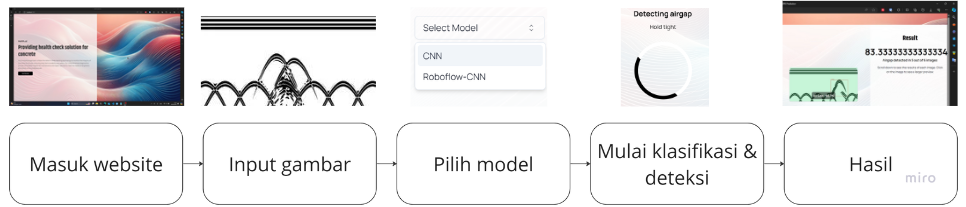
\includegraphics[scale=0.1]{gambar/bab3/flowuser.png}
    \caption{Flowchart Penggunaan Website}
    \label{fig:flowuser}
  \end{figure}
\end{minipage}

Berdasarkan flowchart diatasa, pengguna dapat mengunjungi laman website https://airgap-detect.vercel.app/ dan memasuki laman utama. Kemudian user dapat memasuki laman deteksi untuk mengunggah gambar sinyal yang ingin dideteksi keberadaan rongga udaranya. Pengguna dapat memilih model yang ingin digunakan antara model CNN 2D atau Roboflow. Setelah memilih model, pengguna dapat memulai proses klasifikasi dan deteksi. Hasil klasifikasi dan deteksi akan ditampilkan diakhir proses dengan gambar sinyal yang tidak memiliki rongga udara akan diberi filter merah dan yang memiliki rongga udara akan memilki filter hijau dengan bounding box dari YOLOv9. Hasil tersebut dapat didownload dalam bentuk zip. Website ini dideploy pada vercel dan dihosting dengan biznet. Pada pembuatan website, proses terbagi menjadi dua tahap utama yakni frontend dan backend. Berikut ini adalah flowchart tentang bagaimana website ini bekerja sebagaimana dapat dilihat pada gambar \ref{fig:webflow}.

\begin{minipage}{\linewidth}
  \begin{figure} [H] \centering
    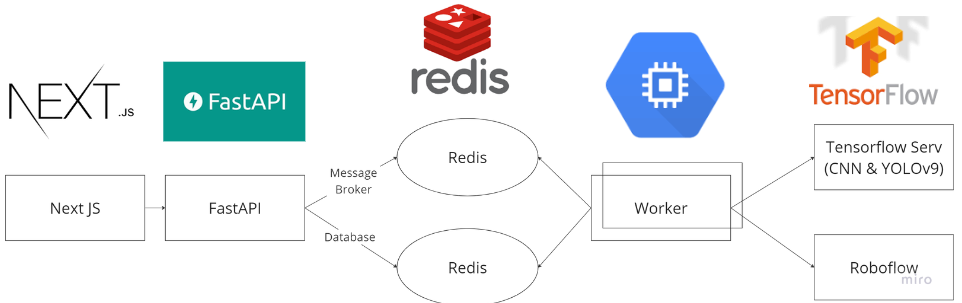
\includegraphics[scale=0.15]{gambar/bab3/webflow.png}
    \caption{Flowchart Website}
    \label{fig:webflow}
  \end{figure}
\end{minipage}

Tahap pertama yang perlu dilakukan adalah pengerjaan bagian frontend. Langkah pertama yang dilakukan adalah melakukan desain dari website tersebut. Proses desain dilakukan pada platform figma. Setelah desain selesai, langkah selanjutnya adalah melakukan implementasi desain tersebut ke dalam kode program. Proses implementasi ini dilakukan dengan menggunakan framework Next.js. Pada tahap ini, dilakukan pembuatan beberapa halaman website yang terdiri dari halaman utama, halaman upload gambar, halaman hasil klasifikasi, dan halaman hasil deteksi. Backend dibuat setelah frontend selesai dimana diperlukan pembuatan API agar frontend dapat bekerja. API yang digunakan pada pembuatan backend adalah FastAPI. FastAPI sendiri digunakan agar website dapat memproses berbagai lebih dari satu user request pada saat yang bersamaan. API ini nantinya akan terhubung dengan Redis sebagai platform database dan message broker yang mana akan menjadi perantara bagi frontend dengan virtual machine yang digunakan untuk melakukan klasifikasi dan deteksi. ketika pengguna mengunggah gambar, maka gambar akan disimpan sementara pada database Redis. Kemudian Redis akan mengirim pesan pada virtual machine sebagai worker untuk melakukan klasifikasi dan deteksi. Sebelumnya, model CNN 2-Dimensi dan YOLOv9 tidak dimasukkan ke dalam virtual machine, melainkan ke dalam Tensorflow Serving. Hal tersebut bertujuan agar model dapat diakses oleh lebih dari satu instance saat terdapat lebih dari satu request dan mengurangi jumlah memori yang akan digunakan oleh setiap instance. Model dari YOLOv9 perlu dikonversi terlebih dahulu dari pytorch ke keras (pb) agar bisa digunakan. Untuk model dari Roboflow, tidak perlu diletakkan pada Tensorflow Serving karena cukup dengan memanggil endpoint saja. Setelah model berhasil diakses, maka model akan melakukan klasifikasi dilanjut dengan deteksi YOLOv9. Hasil klasifikasi dan deteksi tersebut akan dikirimkan ke database untuk dikirimkan kembali ke user serta menghapus gambar yang telah diunggah. Berikut ini adalah contoh hasil dari website yang telah dibuat:

\begin{minipage}{\linewidth}
  \begin{figure} [H] \centering
    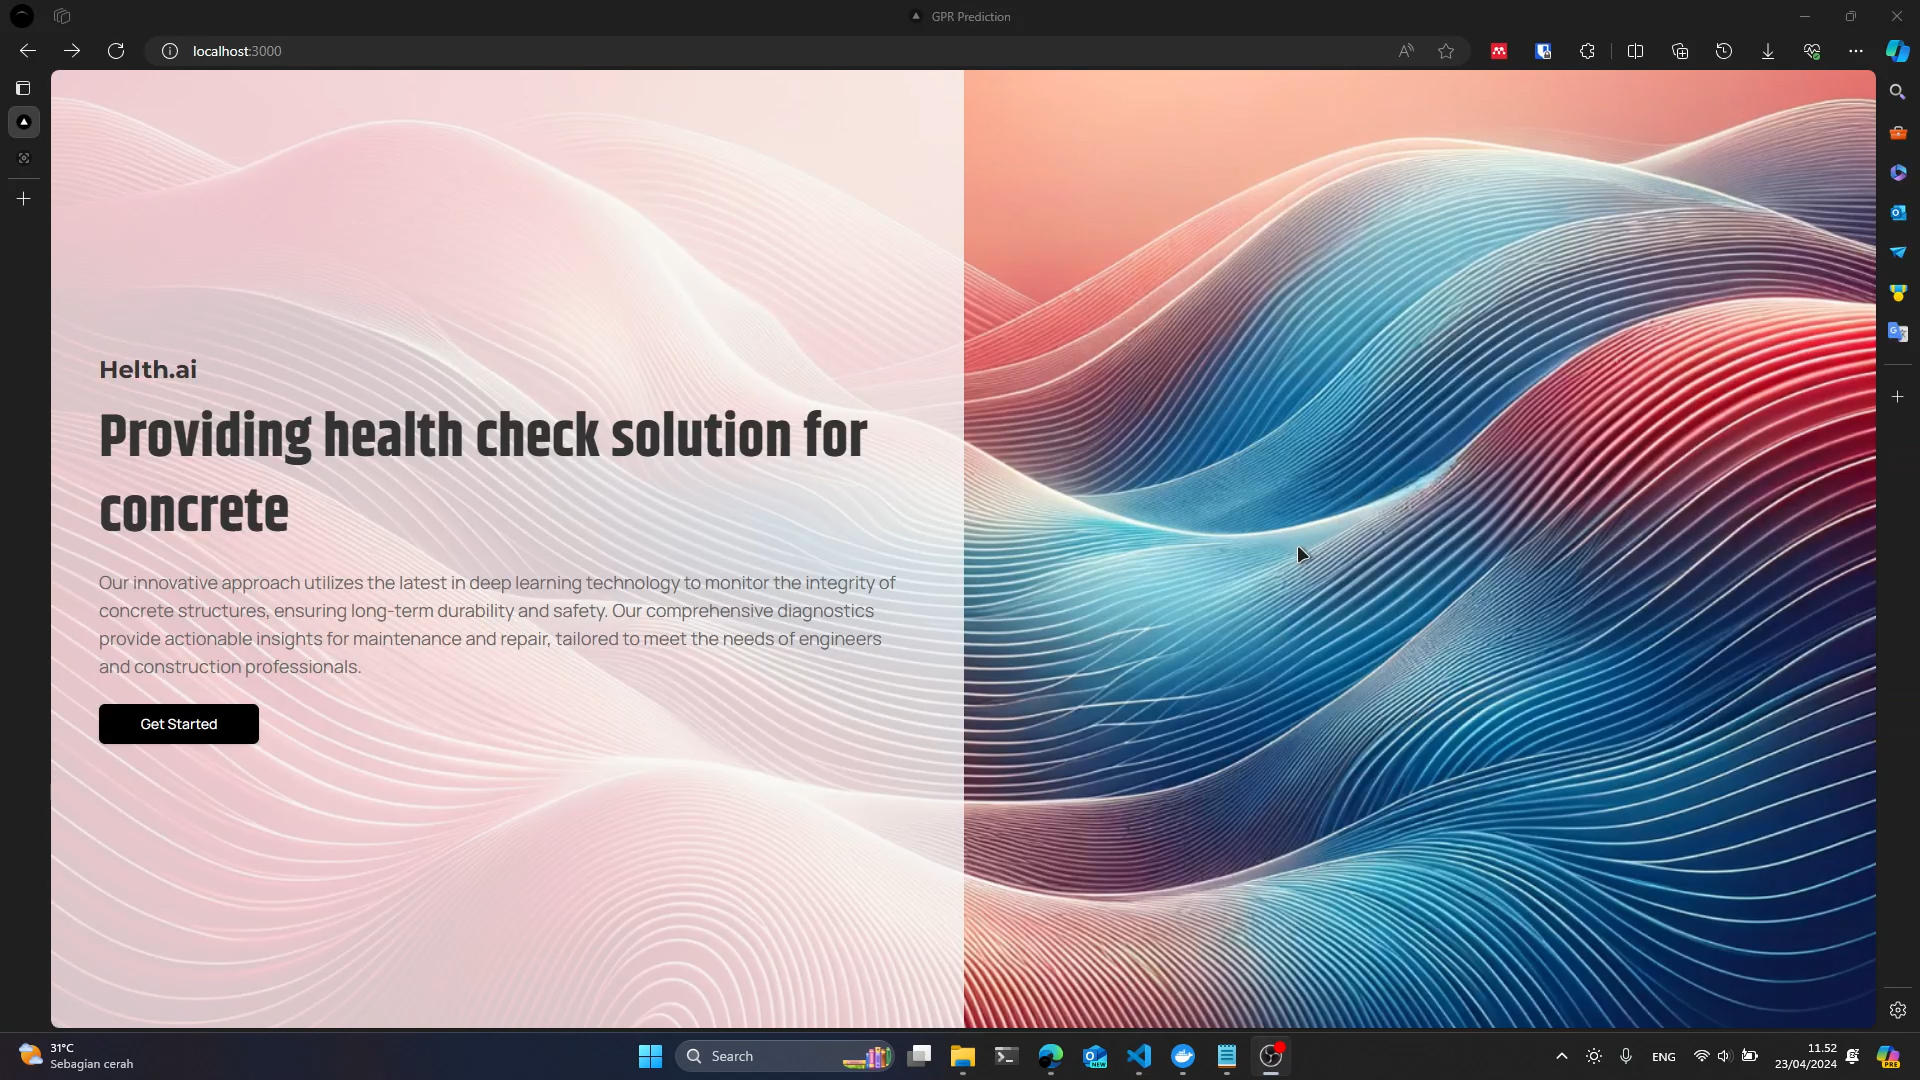
\includegraphics[scale=0.15]{gambar/bab3/web1.png}
    \caption{Gambar Platform Website 1}
  \end{figure}
\end{minipage}

\begin{minipage}{\linewidth}
  \begin{figure} [H] \centering
    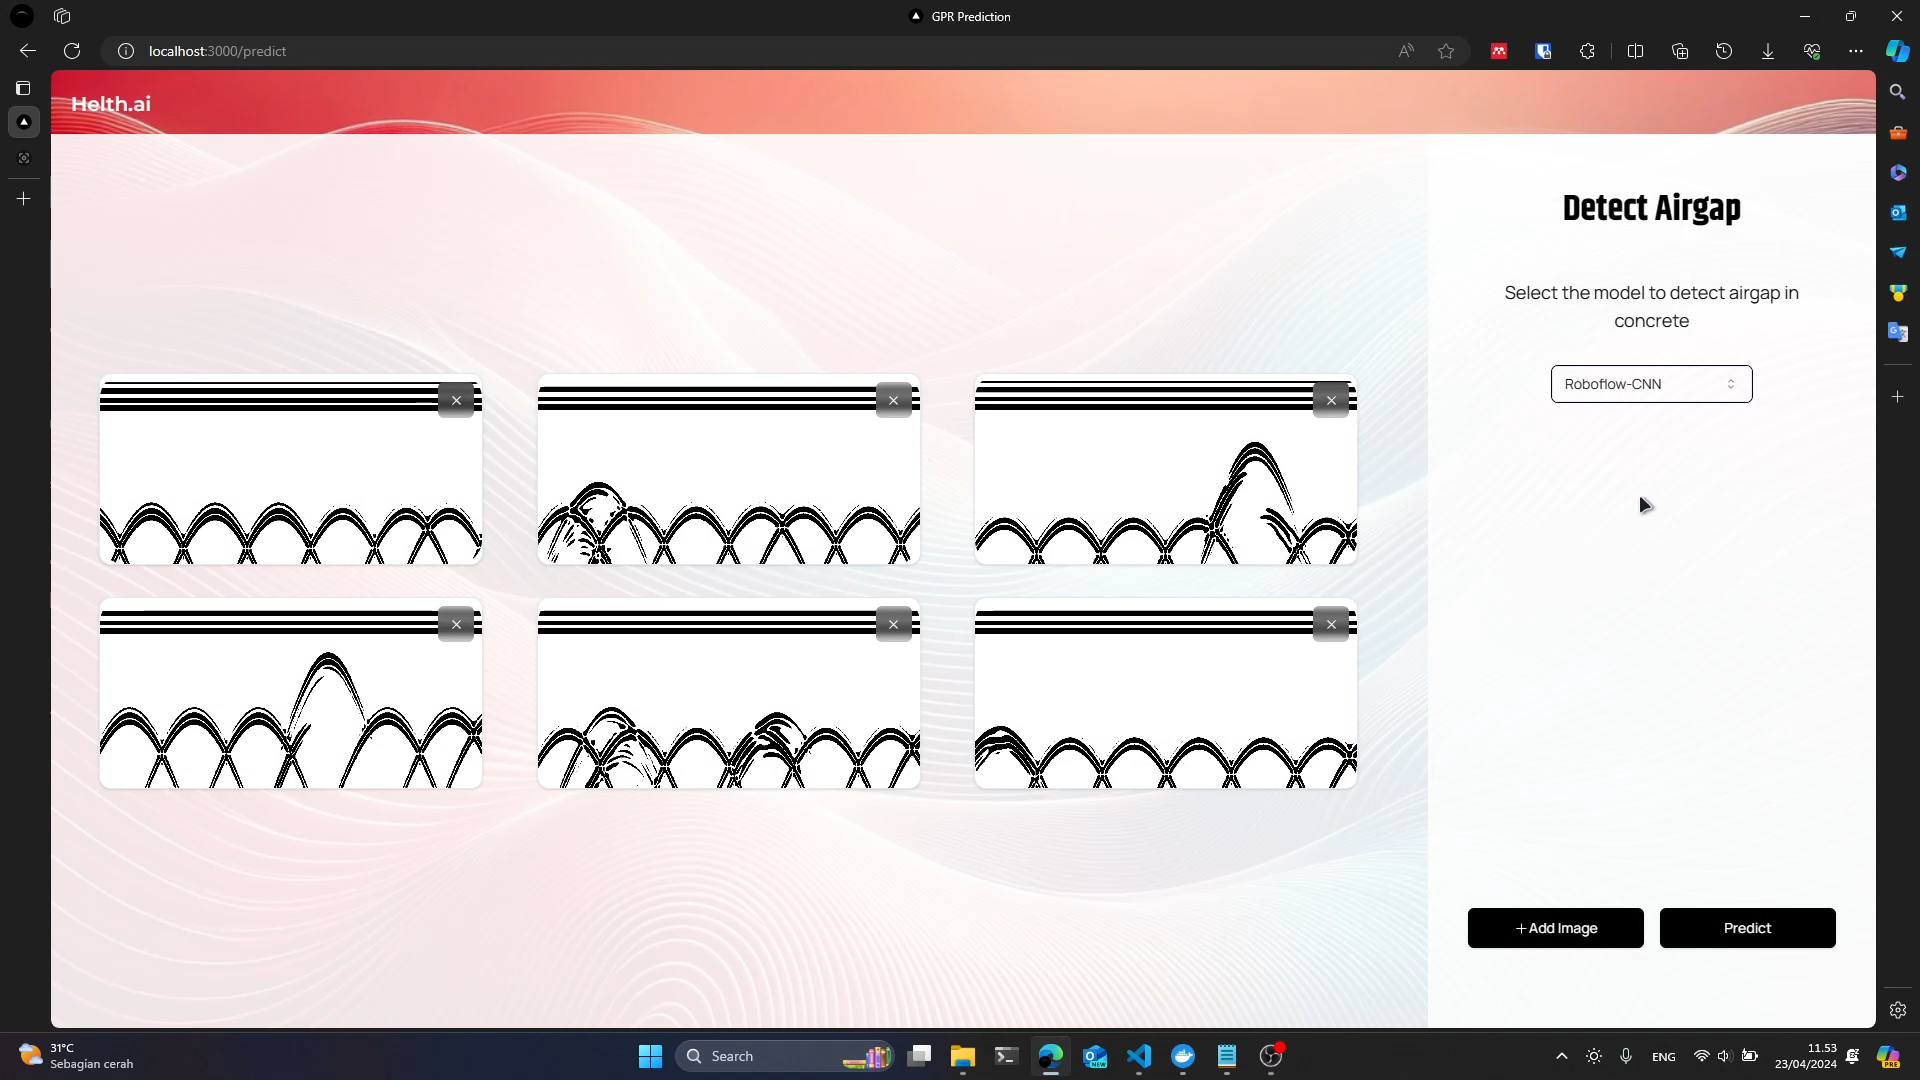
\includegraphics[scale=0.15]{gambar/bab3/web2.png}
    \caption{Gambar Platform Website 2}
  \end{figure}
\end{minipage}

\begin{minipage}{\linewidth}
  \begin{figure} [H] \centering
    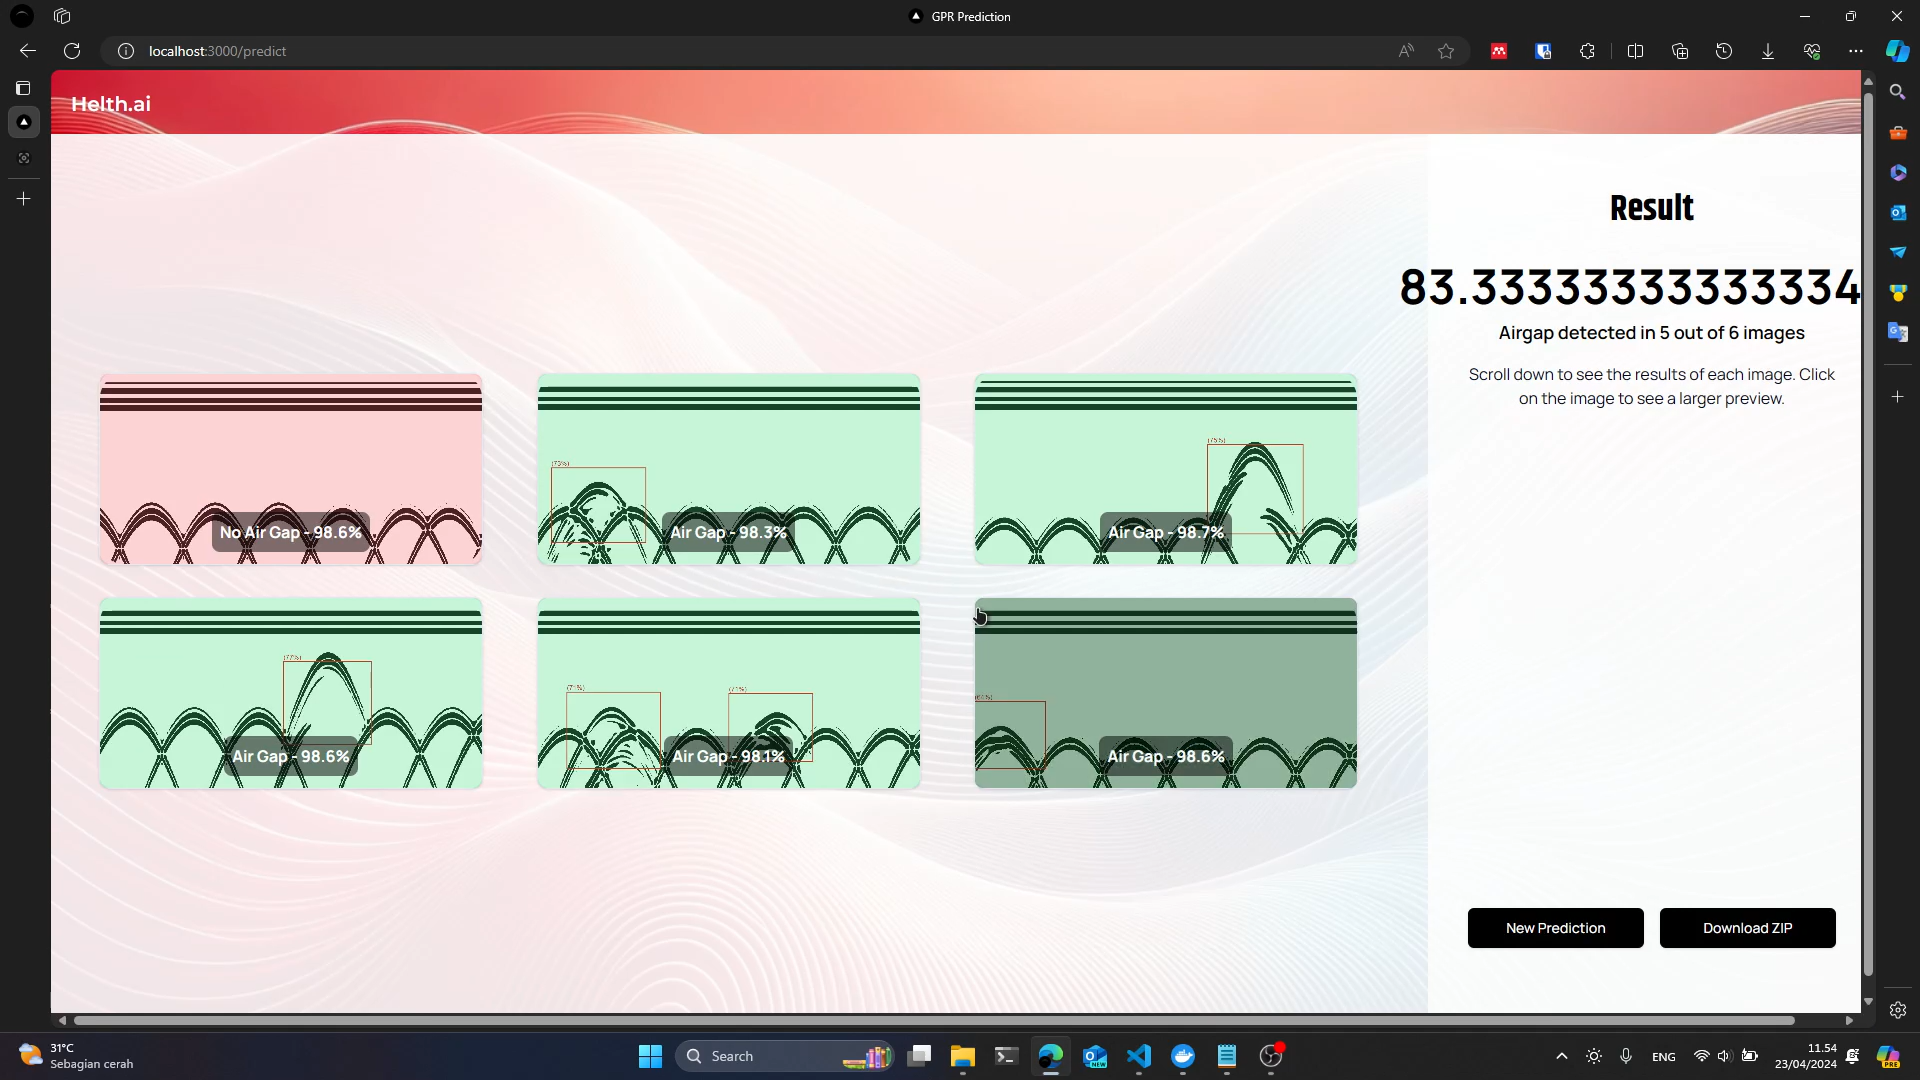
\includegraphics[scale=0.15]{gambar/bab3/web3.png}
    \caption{Gambar Platform Website 3}
  \end{figure}
\end{minipage}

\section{Kode Program}
Pada sub bab ini akan dijabarkan kode program yang digunakan pada penelitian ini.

\subsection{File Input Generate Data}
Gambar sinyal dihasilkan dengan memasukkan file input yang berisi parameter-parameter yang diperlukan untuk menghasilkan gambar sinyal. File input berisi parameter-parameter yang diperlukan untuk menghasilkan gambar sinyal. File input dihasilkan secara otomatis menggunakan python karena jumlahnya yang banyak. Berikut ini adalah flowchart dari file input generate data yang dapat dilihat pada gambar \ref{fig:generateflow}.

\begin{minipage}{\linewidth}
  \begin{figure} [H] \centering
    
\includegraphics[scale=0.1]{gambar/bab3/generateflow.png}
    \caption{Input File Generate Data}
    \label{fig:generateflow}
  \end{figure}
\end{minipage}

\begin{algorithm}
  \caption{Simulation of B-scan from Rebar in Concrete}
  \begin{algorithmic}[1]
      \State Title: "B-scan from rebar in concrete"
      \State Define domain: 1.0 m x 0.3 m x 0.001 m
      \State Cell size: 0.001 m x 0.001 m x 0.001 m
      \State Time window: $3 \times 10^{-9}$ s
      
      \State Define material concrete: $\epsilon=7.0$, $\sigma=0.0$, $\mu=1.0$, $\chi=0.0$
      \State Define material steel: $\epsilon=12.0$, $\sigma=1.0e6$, $\mu=1.0$, $\chi=0.0$
      
      \State Create waveform: Ricker, peak frequency $4.5 \times 10^9$, name "my\_ricker"
      \State Source steps: 0.001 m x 0 m x 0 m
      \State Receiver steps: 0.001 m x 0 m x 0 m
      \State Place box: Start (0.0, 0.0, 0.0), End (1.0, 0.203, 0.001), Material concrete
      
      \State Add Hertzian dipole: Position (0.010, 0.203, 0), Waveform "my\_ricker"
      \State Place receiver: Position (0.050, 0.203, 0)
      
      \State Place cylinders: Positions and dimensions specified for steel
      \State Place cylinders: Positions and dimensions specified for free space
  \end{algorithmic}
\end{algorithm}

Pada awal program, dituliskan judul dari gelombang yang akan dihasilkan yang mana bersifat opsional. Langkah selanjutnya adalah ditentukan ukuran media yang akan dijadikan sebagai simulasi. Pada program juga diinputkan kode untuk menentukan waktu yang akan diamati pada saat berlangsungnya simulasi dan menyusun tingkat satuan terkecil untuk file input. Pada gprMax, terdapat dua material bawaan yakni udara dan \emph{pec} yang merupakan konduktor material sempurna. Pada program ini, ditentukan material yang akan digunakan pada simulasi seperti rebar dan beton yang mana parameternya diambil berdasarkan penelitian terdahulu yang menggunakan gprMax.

Langkah selanjutnya diatur tipe gelombang yakni Ricker wavelet yang mana merupakan gelombang yang paling sering digunakan pada simulasi GPR. Diatur pula letak \emph{transmitter} dan \emph{receiver} yang akan digunakan pada simulasi yang ketinggiannya sama dengan ketinggian/ketebalan dari beton yang akan dibuat. Pergerakan dari \emph{transmitter} dan \emph{receiver} diatur untuk mampu berpindah posisi hingga sekecil 1 mm per langkah. Hal ini dilakukan untuk mendapatkan data sinyal yang lebih banyak dan akurat. Terakhir, ditentukan objek yang nantinya akan ada didalam simulasi seperti beton, rebar, dan rongga udara yang mana masing-masing objek memiliki parameter tersendiri. Pada program ini, beton menggunakan parameter \#box karena medianya kotak, rebar menggunakan parameter \#cylinder karena medianya silinder, dan rongga udara menggunakan parameter \#cylinder rongga udara memiliki bentuk yang abstrak.

\subsection{Generate File Input gprMax dengan Rongga Udara}
Program ini dirancang untuk melakukan proses generate file input gprMax dengan rongga udara. Hal tersebut dilakukan karena proses pembuatan file input gprMax dengan rongga udara dalam jumlah besar membutuhkan waktu yang lama. Program ini dibuat dengan menggunakan Python, berikut ini adalah flowchart tentang bagaimana program ini bekerja sebagaimana dapat dilihat pada gambar \ref{fig:flowgpu}.

\begin{figure} [H] \centering
  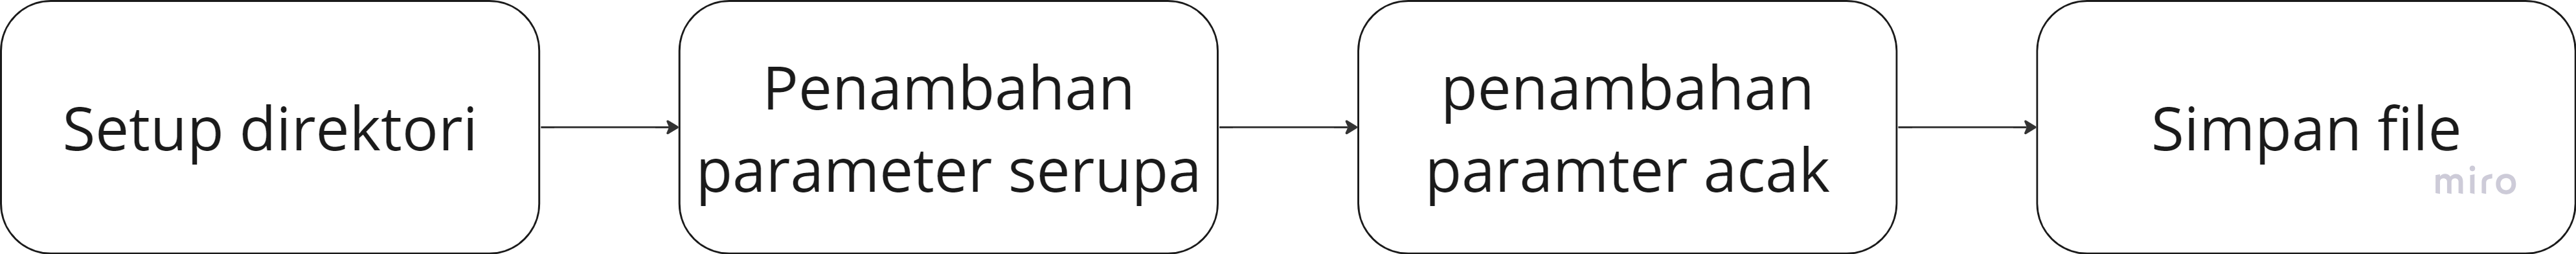
\includegraphics[scale=0.1]{gambar/bab3/flowmakein.png}
  \caption{Flowchart Setup GPU}
  \label{fig:flowmakein}
\end{figure}

\begin{algorithm}
  \caption{Generate gprMax Simulation Files}
  \begin{algorithmic}[1]
  \Function{GenerateAirgapCylinders}{$file, boxHeight$}
      \State $xMin, xMax \gets 0.05, 0.95$
      \State $yMin, yMax \gets 0.090, boxHeight - 0.05$
      \State $airgapCount \gets$ Random integer from 1 to 2
      \For{$i \gets 1$ \textbf{to} $airgapCount$}
          \State $cylinderCount \gets$ Random integer from 3 to 5
          \State $xPosition \gets$ Random float between $xMin$ and $xMax$
          \State $yPosition \gets$ Random float between $yMin$ and $yMax$
          \For{$j \gets 1$ \textbf{to} $cylinderCount$}
              \State $radius \gets$ Random float from 0.005 to 0.0175
              \State Write cylinder data to $file$
              \State Adjust $xPosition$ and $yPosition$ within bounds
          \EndFor
      \EndFor
  \EndFunction
  \State
  \Function{GenerateGprMaxFiles}{}
      \State Create directory "airgap"
      \State $totalFiles \gets 2000$
      \For{$fileNumber \gets 1$ \textbf{to} $totalFiles$}
          \State $boxHeight \gets$ Random float between 0.190 and 0.210
          \State Create file with initial configuration
          \State Write steel cylinder configuration to file
          \State \Call{GenerateAirgapCylinders}{$file, boxHeight$}
          \State Print file creation message
      \EndFor
  \EndFunction
  \end{algorithmic}
  \end{algorithm}

Pada langkah awal, dilakukan inisialisasi dengan membuat folder baru sebagai tempat disiapkannya hasil generate file input gprMax. Kemudian, dilakukan perulangan untuk membuat file text yang berisi struktur dari sinyal yang akan digenerate. Program akan menambahkan parameter-parameter yang akan dimiliki oleh semua file input (parameter serupa) terlebih dahulu di awal seperti judul file, ukuran domain, rentang waktu, tingkat kerincian, mterial, jenis gelombang, dan pergerakan dari transmitter dan receiver gelombang. Setelah itu, dilakukan penambahan baris kode dengan parameter yang sifatnya akan divariasi secara acak. Parameter awal adalah dimensi beton yang berukuran panjang 1 meter variasi ketebalan antara 19 cm hingga 21 cm. Ketebalan dari beton ini akan menentukan posisi ketinggian dari transmitter dan receiver yang akan ditambahkan setelahnya. Selanjutnya, akan ditambahkan parameter rebar yang memiliki material besi dengan diameter 14 mm dengan setiap rebar akan memiliki ketinggian yang sama. Ketinggian dan posisi secara horizontal ini akan berubah setiap filenya dengan rebar memiliki variasi ketinggian antara 9 cm hingga 11 cm sementara posisi horizontal rebar akan bertambah sebanyak 1 mm setiap filenya yang mana apabila posisi rebar secara horizontal melebihi panjang rebar, maka kelebihan posisi tersebut akan ditempatkan pada awal posisi beton secara horizontal. Terkahir adalah parameter rongga udara yang akan ditempatkan secara acak pada beton. Rongga udara udara bisa terdiri dari satu atau lebih silinder dengan diameter antara 2 cm hingga 7 cm yang letak ketinggiannya akan berada diantara 5 cm hingga titik tertinggi beton dikurangi 5 cm. Posisi rongga udara secara horizontal akan diletakkan secara acak. Setelah semua parameter ditambahkan, file akan disimpan dalam format .in.

\subsection{Setup GPU untuk Generate Data}
Dalam, penggunaan GPU untuk mempercepat proses generate data, diperlukan pengaturan GPU terlebih dahulu agar GPU dapat digunakan. Berikut ini adalah flowchart dari setup GPU untuk generate data yang dapat dilihat pada gambar \ref{fig:flowgpu}.

\begin{figure} [H] \centering
  
\includegraphics[scale=0.1]{gambar/bab3/flowgpu.png}
  \caption{Flowchart Setup GPU}
  \label{fig:flowgpu}
\end{figure}

\begin{algorithm}
\caption{Setup Miniconda and Configure gprMax Environment}
\begin{algorithmic}[1]
\State Echo "Creating Miniconda directory..."
\State Execute "mkdir -p \textasciitilde/miniconda3"
\State Echo "Downloading Miniconda installer..."
\State Execute "wget https://repo.anaconda.com/miniconda/Miniconda3-latest-Linux-x86\_64.sh -O \textasciitilde/miniconda3/miniconda.sh"
\State Echo "Installing Miniconda..."
\State Execute "bash \textasciitilde/miniconda3/miniconda.sh -b -u -p \textasciitilde/miniconda3"
\State Echo "Removing Miniconda installer..."
\State Execute "rm -rf \textasciitilde/miniconda3/miniconda.sh"
\State Echo "Initializing Conda for bash..."
\State Execute "\textasciitilde/miniconda3/bin/conda init bash"
\State Execute "source ./\.bashrc"
\State Echo "Updating Conda..."
\State Execute "conda update conda -y"
\State Echo "Installing Git..."
\State Execute "conda install git -y"
\State Echo "Cloning gprMax repository..."
\State Execute "git clone https://github.com/MaulanaGilang/gprMax.git"
\State Echo "Changing directory to gprMax..."
\State Execute "cd gprMax"
\State Echo "Creating Conda environment from file..."
\State Execute "conda env create -f conda\_env.yml"
\State Echo "Activating gprMax environment..."
\State Execute "conda activate gprMax"
\State Echo "Building gprMax..."
\State Execute "python setup.py build"
\State Echo "Installing gprMax..."
\State Execute "python setup.py install"
\State Echo "Installing PyCUDA..."
\State Execute "pip install pycuda
\State Echo "Setup complete. gprMax is ready to use."
\end{algorithmic}
\end{algorithm}

Pada awal pengaturan GPU, GPU diakses melalui ssh yang terhubung dengan ssh key milik PC penulis. Setelah terhubung, dibuat folder baru untuk instalasi miniconda. Instalasi miniconda dilakukan dengan melakukan replikasi repositori github dan menjalankan file bash yang ada pada repositori tersebut. Setelah instalasi selesai, dilakukan pembaruan terhadap versi conda dan intalasi Git untuk proses instalasi gprMax. Proses instalasi gprMax dilakukan dengan melakukan replikasi repositori Github. Sebelum, menjalankan instalasi, dibuat environment baru untuk gprMax dan mengaktifkannya. Setelah aktif, dijalankan kode python dari repositori tersebut untuk melakukan setup gprMax. Langkah terakhir adalah melakukan instalasi PyCUDA agar proses generate data dapat menggunakan GPU.

\subsection{Generate Data Sinyal GPR}
Program ini dirancang untuk melakukan proses generate sinyal hasil simulasi file input untuk gprMax. Program ini dibuat dengan menggunakan python dan menggunakan library gprMax untuk menghasilkan data sinyal. Program ini akan menghasilkan data sinyal berupa gambar B-Scan 2 dimensi yang kemudian akan dijadikan sebagai data training untuk klasifikasi. Berikut ini adalah flowchart dari generate data yang dapat dilihat pada gambar \ref{fig:autoflow} dan \ref{fig:generatefloor}.

\begin{minipage}{\linewidth}
  \begin{figure} [H] \centering
    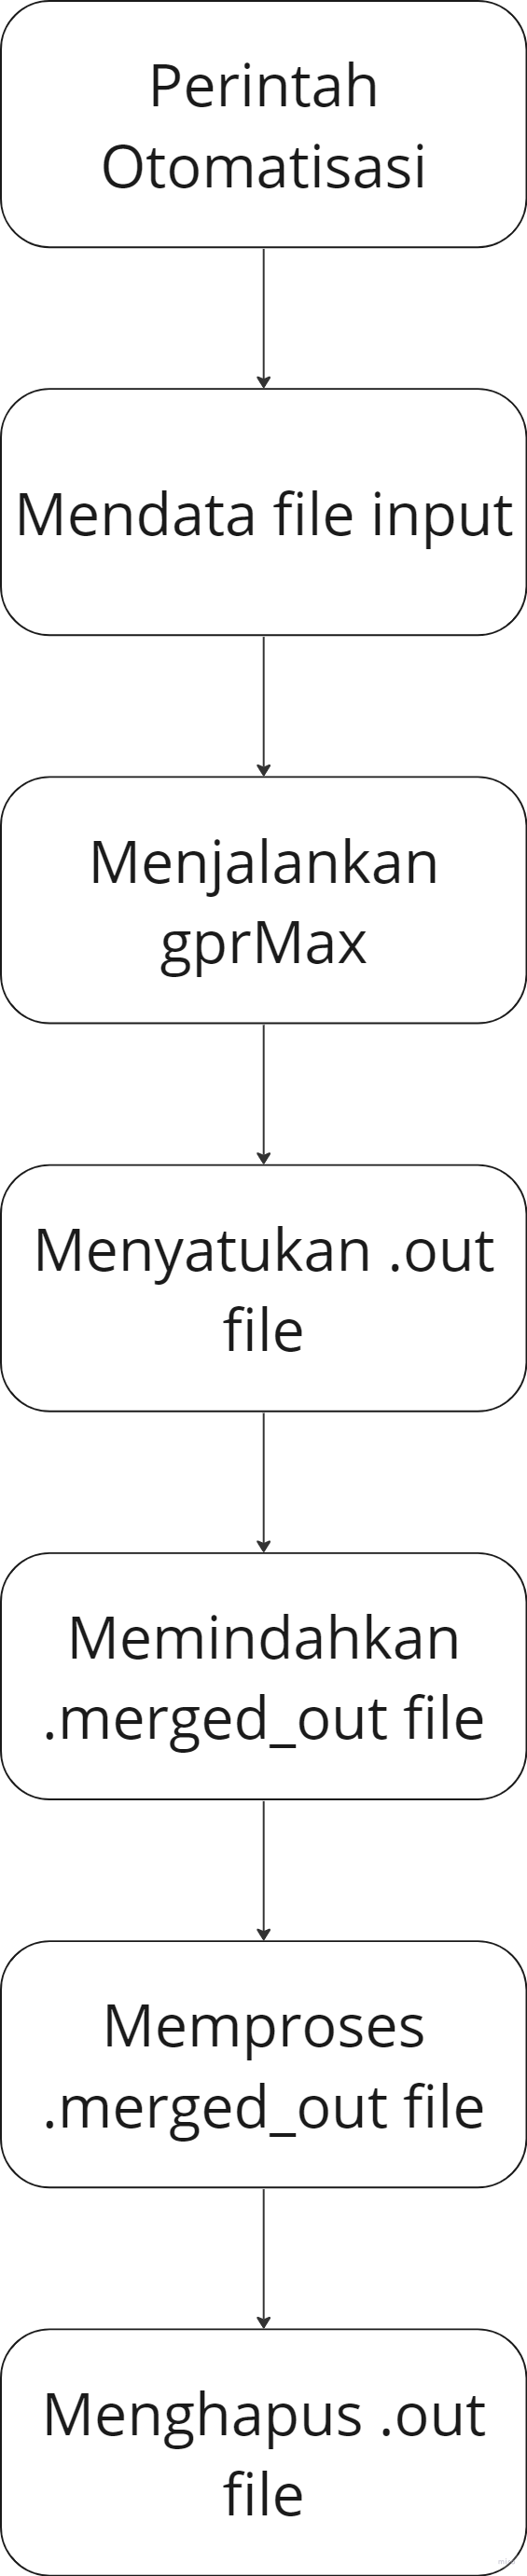
\includegraphics[scale=0.1]{gambar/bab3/autoflow.png}
    \caption{Kode Otomatiasi Generate Data}
    \label{fig:autoflow}
  \end{figure}
\end{minipage}

\begin{algorithm}
  \caption{Process GPRMax Output Files}
  \begin{algorithmic}[1]
  \Function{NaturalKeys}{text}
      \State Parse text and return parts as integers if they are digits or as text otherwise.
  \EndFunction
  \State
  \Function{ListInFilesRecursive}{directory}
      \State Recursively list all .in files in the directory.
      \State Return a dictionary of filenames without extension as keys and paths as values.
  \EndFunction
  \State
  \Function{RunGprMax}{file\_path, n, use\_gpu}
      \State Construct and run a command to execute gprMax with optional GPU usage.
  \EndFunction
  \State
  \Function{MergeOutputFiles}{directory, file\_without\_ext}
      \State Merge output files based on the .in filename and delete the original .out files.
  \EndFunction
  \State
  \Function{EnsureDirectoryExists}{directory}
      \State Create the directory if it does not exist.
  \EndFunction
  \State
  \Function{MoveOutputFile}{source\_path, dest\_directory}
      \State Move the output file to a specified directory, ensuring the directory exists.
      \State Return the new path.
  \EndFunction
  \State
  \Function{ProcessFile}{file\_path, rxnumber, rxcomponent, non\_greyscale\_dir, greyscale\_dir}
      \State Generate and save color and cropped grayscale images from the output data of gprMax.
  \EndFunction
  \State
  \Procedure{Main}{args}
      \State Parse input directory, indices and settings from command-line arguments.
      \State Initialize directories and prepare file processing.
      \For{each file to process within index range}
          \State Run gprMax simulation.
          \If{merge is enabled}
              \State Merge output files.
              \State Move and process merged file.
          \EndIf
          \State Increment processed files count.
      \EndFor
      \State Clean up any remaining processed files.
  \EndProcedure
  \end{algorithmic}
  \end{algorithm}

Pada program ini, pertama-tama dilakukan import library yang dibutuhkan. Selanjutnya, dilakukan pembacaan file input yang telah dibuat sebelumnya. File input tersebut berisi parameter-parameter yang diperlukan untuk menghasilkan gambar sinyal. Setelah itu, program akan melakukan iterasi sebanyak jumlah data yang diinginkan. Pada setiap iterasi, program akan menghasilkan gambar sinyal berdasarkan parameter yang ada pada file input dengan menjalankan software gprMax. Saat setelah selesai generate, setiap file input akan menghasilkan file output berupa potongan-potongan sinyal dengan format .out yang akan disatukan menjadi satu file dengan format .merged.out File ini kemudian akan dipindahkan ke folder yang telah disediakan dan akan menghapus semua file awal berformat .out untuk mengurangi memori yang digunakan oleh GPU. File yang dipindahkan tersebut akan dibaca dan diubah menjadi gambar sinyal menggunakan python. Gambar sinyal yang telah dihasilkan kemudian akan diproses agar parameter bawaan gambar dari gprMax hilang dan hanya menampilkan gambar sinyal saja serta memotong ukuran gambar tersebut.

\begin{minipage}{\linewidth}
  \begin{figure} [H] \centering
    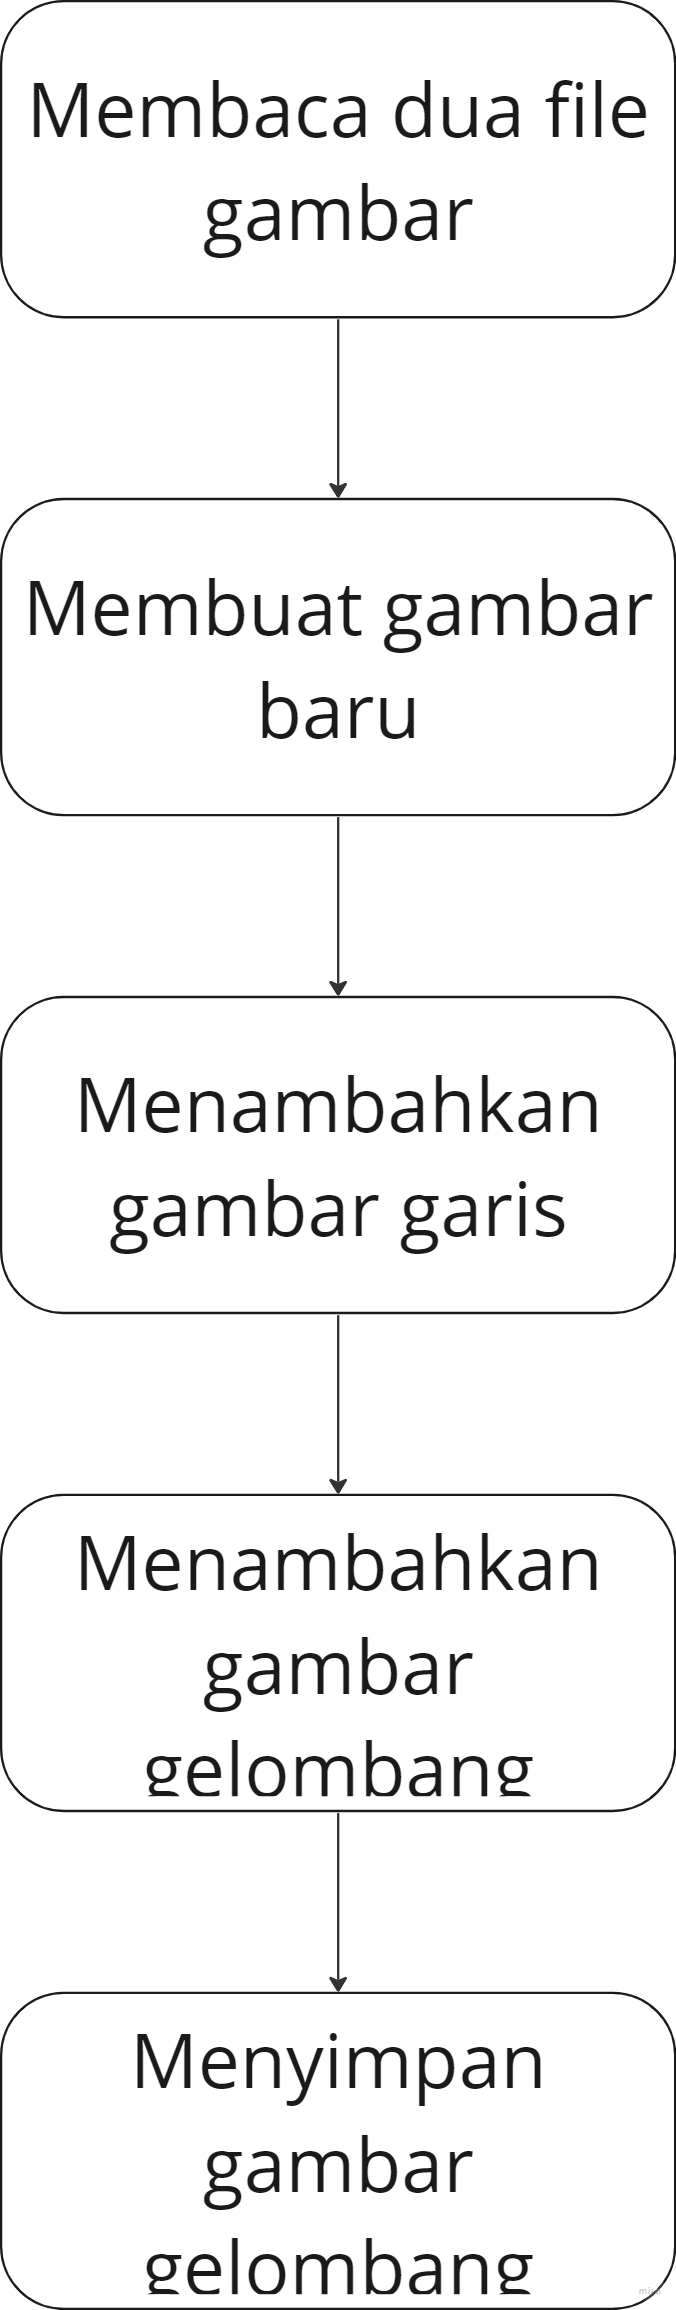
\includegraphics[scale=0.1]{gambar/bab3/generatefloor.png}
    \caption{Input File Generate Data}
    \label{fig:generatefloor}
  \end{figure}
\end{minipage}

\begin{algorithm}
  \caption{Image Manipulation and Transformation}
  \begin{algorithmic}[1]
  \State Load line and wave images from 'noairgap' directory.
  \State Create a new transparent RGBA image 'result\_img' with dimensions 1860x1160.
  \State Paste the line image onto 'result\_img' at position (0,0).
  
  \Function{TransformAndSave}{wave\_img, result\_img, shift\_x, shift\_y, crop\_size, file\_name}
      \State Create a copy of 'result\_img' to 'temp\_img'.
      \State Paste 'wave\_img' onto 'temp\_img' with specified shifts 'shift\_x' and 'shift\_y'.
      \State Repaste the line image onto 'temp\_img' at position (0,0).
      \State Crop 'temp\_img' according to 'crop\_size'.
      \State Save the cropped image to 'file\_name'.
  \EndFunction
  
  \State Calculate number of images to be generated.
  \State Initialize a counter to zero.
  \For{each horizontal shift from -wave width + 1860 to 0 step by 5}
      \For{each vertical shift from 0 to 100 step by 20}
          \State Construct file name for output image.
          \State \Call{TransformAndSave}{wave\_img, result\_img, horizontal shift, vertical shift, crop size, file name}
          \State Increment counter by one.
      \EndFor
  \EndFor
  
  \end{algorithmic}
  \end{algorithm}

Untuk program generate data sinyal gprMax yang tidak memiliki rongga udara, data ini dihasilkan dengan cara yang berbeda karena tidak banyak perbedaan pada setiap gambar sinyal yang dihasilkan. Untuk menjalan program ini, dibutuhkan gambar sinyal tanpa rongga udara hasil generate gprMax dengan gambar pertama adalah gambar normal dan gambar kedua adalah gambar sinyal dengan rebar yang memiliki sebuah rebar yang tidak berjarak 15 cm. Selanjutnya, kedua gambar tersebut disatukan secara horizontal dan dipotong bagian sinyalnya. Selanjutnya, diambil gambar garis pada salah satu gambar dengan cara dipotong. Dua gambar tersebut nantinya akan menjadi file input untuk augmentasi tersebut. Pada program, akan dibuat sebuah gambar baru dengan ukuran 1860x1160 piksel dengan latar belakang yang transparan. Kemudian, akan ditambahkan gambar garis pada bagian atas gambar tersebut. Selanjutnya ditambahkan gambar sinyal dibagian bawah gambar garis dengan ketentuan setiap gambar sinyal tersebut akan dipindahkan posisinya per gambar secara horizontal sebanyak 5 piksel hingga menyentuh batas gambar sinyal secara horizontal dan secara vertikal ke bawah 100 piksel dengan perpindahan 20 piksel per gambar. Gambar sinyal dan garis akan menimpa gambar latar belakang sehingga tercipta gambar sinyal baru. Gambar sinyal yang telah dihasilkan nantinya akan disimpan pada folder yang telah disediakan.

\subsection{\emph{Preprocessing} Data}
Program berikut ini bertujuan untuk melakukan \emph{preprocessing} data sinyal yang telah dihasilkan dari proses generate data. Program ini dibuat menggunakan python. Berikut ini adalah flowchart dari \emph{preprocessing} data yang dapat dilihat pada gambar \ref{fig:preflow1} dan \ref{fig:preflow2}

\begin{figure} [H] \centering
  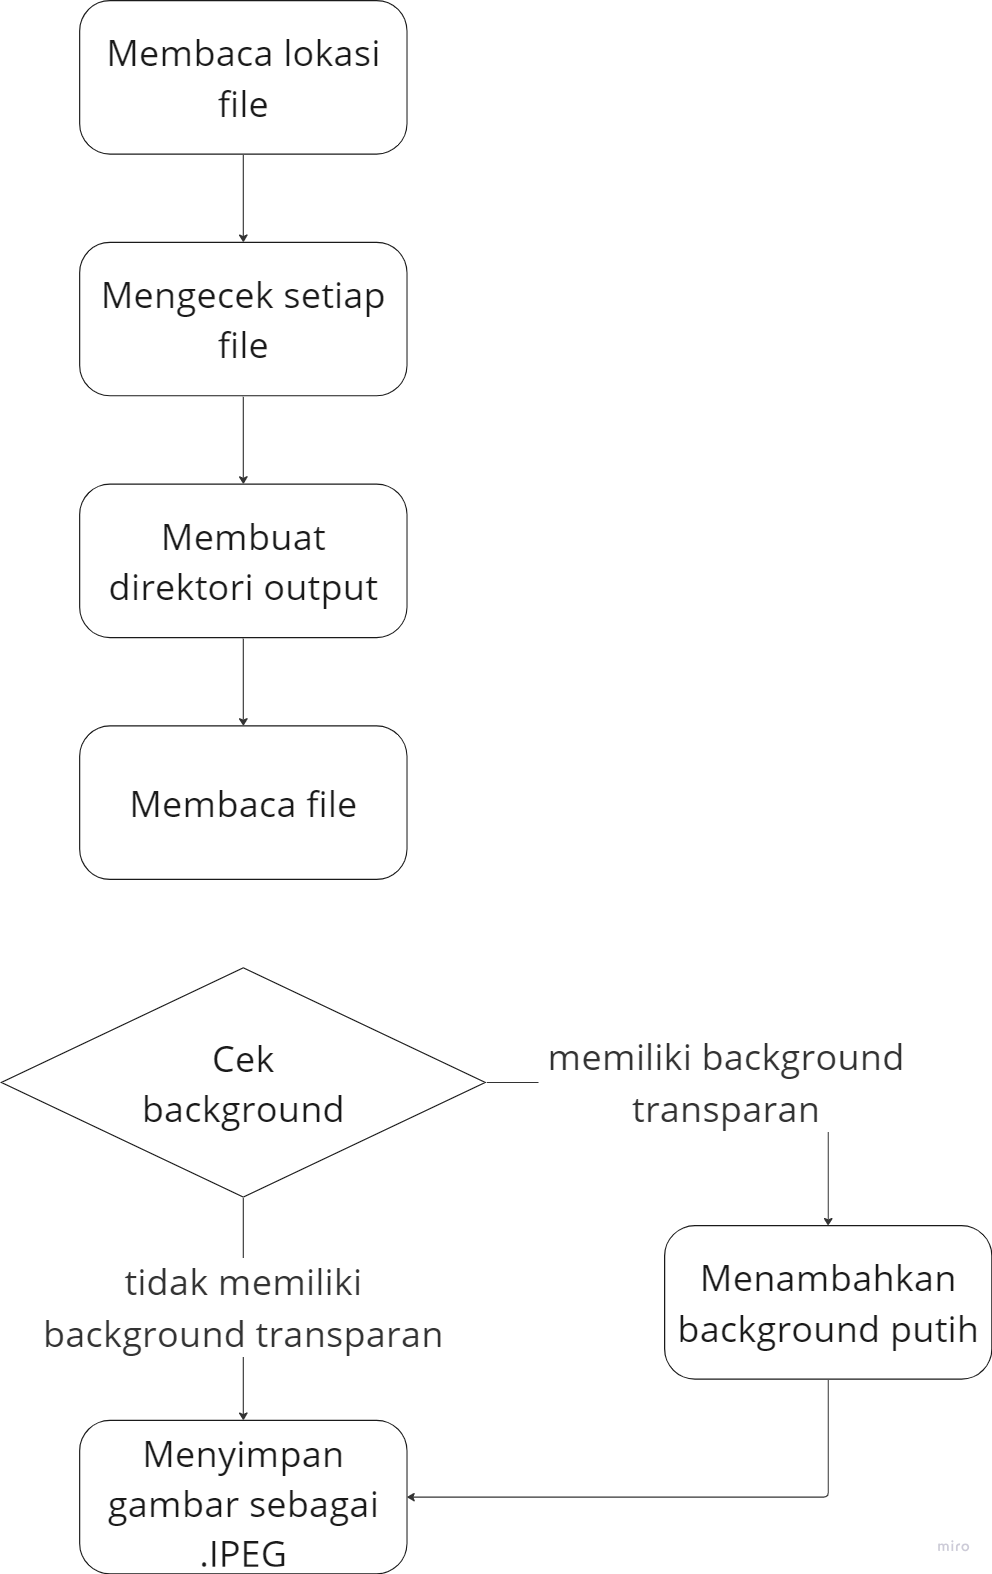
\includegraphics[scale=0.1]{gambar/bab3/preflow1.png}
  \caption{Mengubah Format Gambar Sinyal}
  \label{fig:preflow1}
\end{figure}

\begin{algorithm}
  \caption{Convert Directory Images to JPEG Format}
  \begin{algorithmic}[1]
  \Procedure{ConvertDirectoryToJPEG}{input\_dir, output\_base\_dir}
      \For{each root, dirs, files in input\_dir}
          \For{each file in files}
              \If{file ends with (.png, .jpg, .jpeg, .tiff, .bmp, .gif)}
                  \State Calculate input path
                  \State Calculate relative path from input\_dir
                  \State Define output directory based on relative path
                  \If{output directory does not exist}
                      \State Create output directory
                  \EndIf
                  \State Define output file path with .jpg extension
                  \State Open the image from input path
                  \If{image has alpha channel}
                      \State Create a white background image of same size
                      \State Paste image onto the background using alpha channel as mask
                      \State Set image to the new composite image
                  \EndIf
                  \State Save the image in JPEG format to output file path
                  \State Break loop \Comment{Remove this line to process all files in the directory}
              \EndIf
          \EndFor
      \EndFor
  \EndProcedure
  \end{algorithmic}
\end{algorithm}

Flowchart diatas menjelaskan proses mengubah format gambar sinyal yang dihasilkan dari proses augmentasi python untuk sinyal tanpa rongga udara. Pada program ini, pertama-tama dilakukan pembacaan lokasi file yang ingin diubah formatnya. Kemudian dilakukan import library yang dibutuhkan. Selanjutnya, program akan membaca gambar sinyal yang telah dihasilkan dari proses generate data. Gambar sinyal tersebut kemudian akan diubah formatnya agar dapat diproses. Gambar sinyal yang telah diubah formatnya akan disimpan pada folder yang telah disediakan.

\begin{figure} [H] \centering
  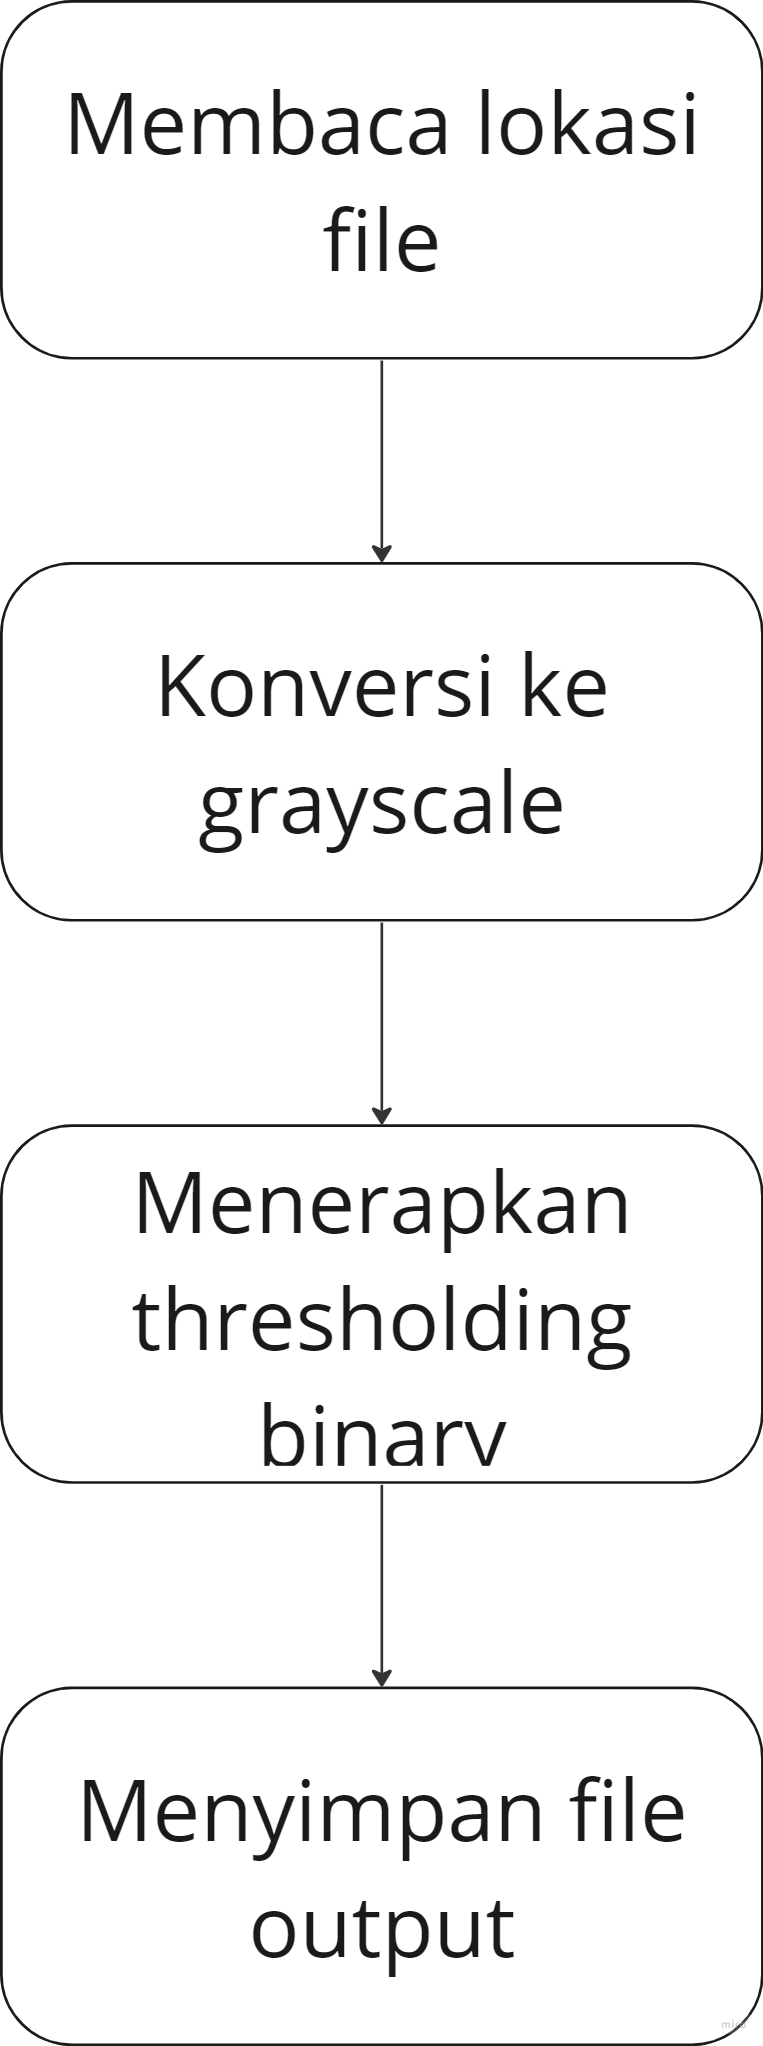
\includegraphics[scale=0.1]{gambar/bab3/preflow2.png}
  \caption{Proses Binarisasi}
  \label{fig:preflow2}
\end{figure}

\begin{algorithm}
  \caption{Process Images in a Directory}
  \begin{algorithmic}[1]
  \Function{ProcessImage}{image\_path, output\_dir}
      \State Read the image from image\_path
      \State Convert the image to grayscale
      \State Apply Otsu's thresholding to the grayscale image to obtain a binary image
      \State Construct the output path relative to output\_dir
      \State Ensure the parent directory of output path exists
      \State Save the binary image to the output path
  \EndFunction
  \State
  \Procedure{ProcessDirectory}{input\_dir, output\_dir}
      \State Convert input\_dir and output\_dir to Path objects
      \State Prepare a list of image files to process, filtering by extensions (.png, .jpg, .jpeg, .bmp)
      \For{each image\_path in the list of image files}
          \State \Call{ProcessImage}{image\_path, output\_dir}
      \EndFor
  \EndProcedure
  \State
  \State Specify the input and output directories
  \State Call \Call{ProcessDirectory}{input\_dir, output\_dir}
  \end{algorithmic}
\end{algorithm}  

Selanjutnya, flowchart diatas menjelaskan proses untuk mengubah gambar menjadi binarisasi. Pada program ini, pertama-tama dilakukan pembacaan lokasi file yang ingin diubah formatnya. Kemudian dilakukan import library yang dibutuhkan. Selanjutnya, program akan membaca gambar sinyal yang telah dihasilkan dari proses generate data. Gambar sinyal tersebut kemudian akan diubah formatnya menjadi grayscale. Setelah itu, diterapkan threshold agar gambar sinyal tersebut menjadi biner. Gambar sinyal yang telah diubah formatnya akan disimpan pada folder yang telah disediakan.

\subsection{\emph{Training} Data}
Pada proses training data menggunakan CNN 2D, perlu dilakukan penyusunan program untuk training CNN 2D pada Google Colab. Berikut ini adalah flowchart dari training data CNN 2D yang dapat dilihat pada gambar \ref{fig:trainingcnn}.

\begin{figure} [H] \centering
  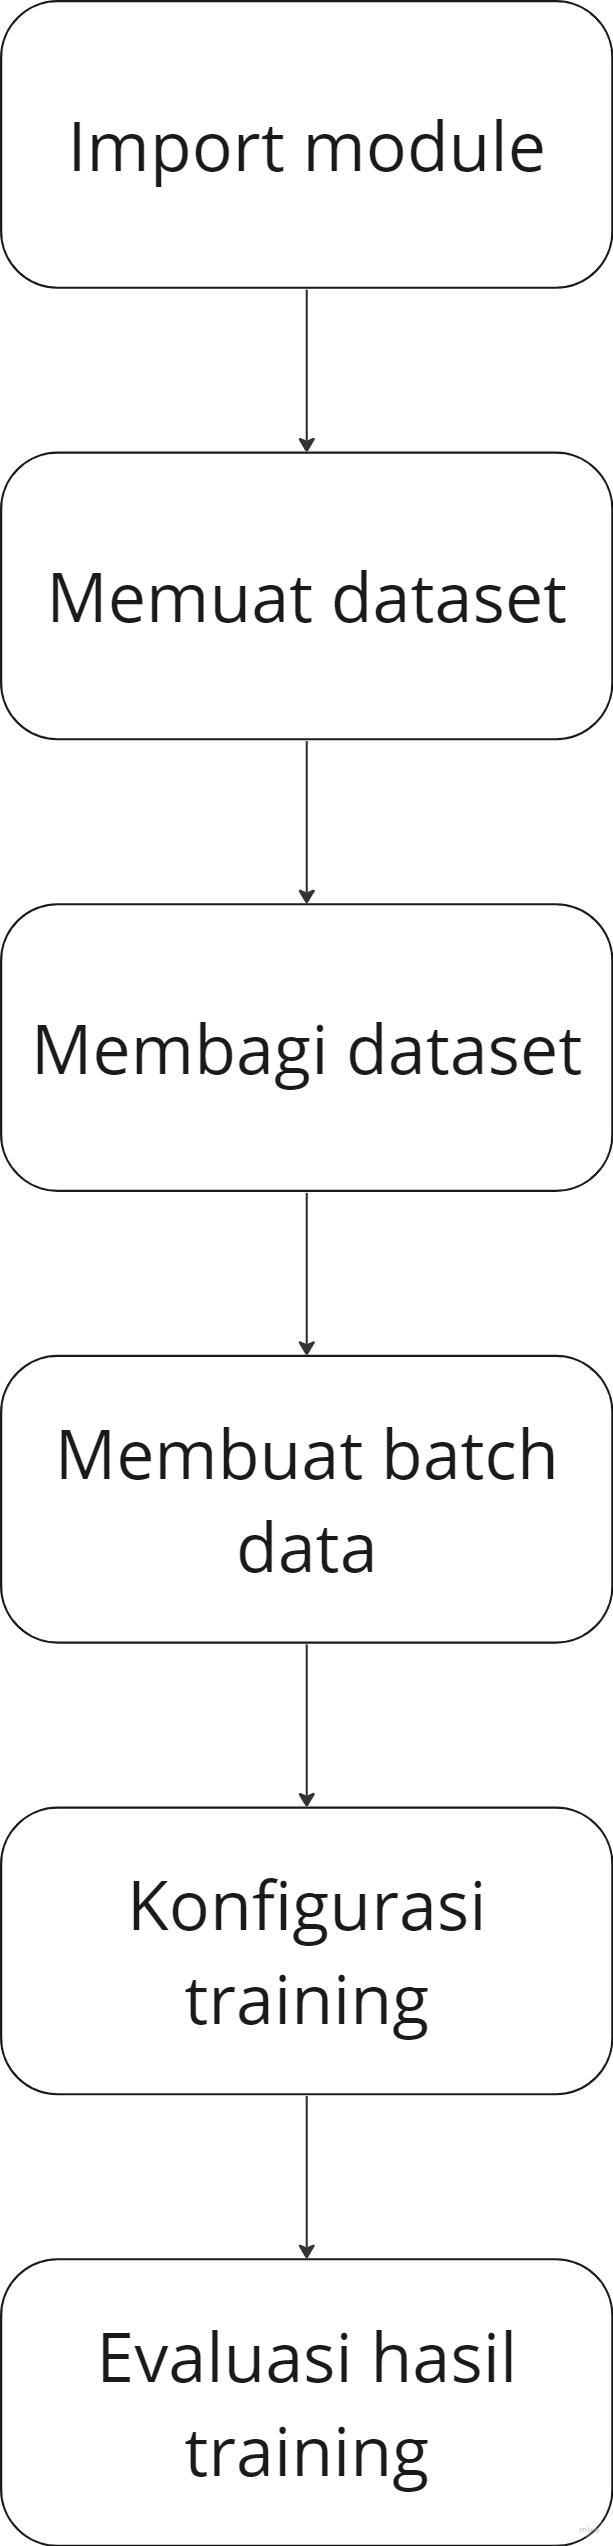
\includegraphics[scale=0.1]{gambar/bab3/trainingcnn.png}
  \caption{Training CNN 2D}
  \label{fig:trainingcnn}
\end{figure}

\begin{algorithm}
  \caption{Training and Evaluation of CNN for Image Classification}
  \begin{algorithmic}[1]
  \State Import necessary modules and libraries
  \State Mount Google Drive and set paths for datasets
  \State Initialize random seeds for reproducibility
  
  \State Define data generators with augmentation settings for training and validation
  \State Prepare data generators for training and validation subsets
  
  \Function{CreateModel}{}
      \State Define a sequential model with multiple convolutional blocks
      \State Add pooling, flattening, dense, and dropout layers
      \State Configure compilation settings (optimizer, loss, metrics)
      \State \textbf{return} model
  \EndFunction
  
  \State Instantiate the model using \Call{CreateModel}{}
  \State Print model summary
  
  \State Define EarlyStopping callback for training
  \State Train model using fit method with callbacks
  \State Evaluate model on validation and training data
  
  \State Plot accuracy and loss graphs for training and validation
  \State Save the trained model to Google Drive
  
  \State Predict on new data using test generators
  \State Display and analyze confusion matrices for training and validation sets
  
  \State Calculate and print F1 scores for training, validation, and test sets
  
  \State Annotate test images with predictions and save outputs
  
  \end{algorithmic}
\end{algorithm}

Pada CNN 2D, digunakan Google Colab sebagai platform untuk training data. Pada CNN ini, digunakan tensorflow untuk mengimport semua kebutuhan CNN 2D. Kemudian mendefinisikan dua generator data gambar, train datagen dan val datagen, yang masing-masing digunakan untuk augmentsi data training secara otomatis dan menyiapkan data validasi. Kedua generator mengubah skala nilai pixel gambar dari [0, 255] menjadi [0, 1] dengan mengalikannya dengan 1,0/255 untuk menormalisasi data. train datagen juga menerapkan transformasi acak seperti geser dan zoom (masing-masing hingga 20\%) dan mengatur fill mode ke "nearest" untuk menangani pixel di luar batas gambar selama transformasi. Generator data ini dikonfigurasi untuk membagi kumpulan data menjadi subset training dan validasi, dengan 20\% data dicadangkan untuk validasi.Kemudian gambar diproses agar sesuai dengan ukuran input model 330x540 piksel, menanganinya dalam 10 batch, dan menghasilkan gambar grayscale. Mode kelas diatur ke "biner" yang menunjukkan bahwa klasifikasi tersebut adalah klasifikasi biner.

Kode CNN ini memiliki variasi dalam layerya. Hal serupa yang dimiliki setiap variasi adalah setiap variasi dari CNN 2-Dimensi memiliki setidaknya sebuah Convolutional layer dan Dense layer yang jumlah serta pengaturan lanjutan yang berbeda-beda pada setiap eksperimen. Kemudian ditambahkan dense layer terakhir dengan unit tunggal dan aktivasi sigmoid untuk klasifikasi biner. Selanjutnya, dilakukan konfigurasi model training dengan menggunakan model.compile() yang mengatur optimizer, loss function, dan metrik evaluasi. Pada model ini, digunakan optimizer Adam dengan loss function binary crossentropy, dan metrik evaluasi akurasi. Kemudian, model dilatih dengan model.fit() yang mengatur generator data training, jumlah epoch sebanyak, generator data validasi, dan langkah validasi. Pada model ini, dilakukan training sebanyak 100 epoch dengan early stopping dan langkah validasi yang disesuaikan dengan ukuran batch dan jumlah validasi. Setelah training selesai, model disimpan dalam format .h5 dan proses training menghasilkan data yang diperlukan terkait hasil training itu sendiri.

Pada percobaan pertama, kedua, dan ketiga, digunakan model CNN 2D yang sama untuk mengetahui pembagian data yang baik. Model pada ketiga percobaan ini dapat dilihat pada tabel \ref{fig:cnnarc1} dimana model ini memiliki total 14 layer dengan rincian 4 Convolutional layer, 4 MaxPooling layer, 1 flatten layer, 2 dropout layer dan 3 dense layer. Untuk percobaaan keempat, digunakan pembagian data yang terbaik dari tiga percobaan pertama. Terdapat perbedaan pada model CNN 2D pada percobaan keempat ini dimana model ini memiliki total 18 layer dengan rincian 4 Convolutional layer, 4 MaxPooling layer, 1 flatten layer, 2 dropout layer, 3 dense layer dan 4 BatchNormalization layer yang ditambahkan setelah setiap Convolutional layer Model pada percobaan keempat ini dapat dilihat pada tabel \ref{fig:cnnarc2}. Sementara itu, pada percobaan kelima, digunakan model CNN 2D dengan layer yang lebih sedikit. Model pada percobaan kelima ini dapat dilihat pada tabel \ref{fig:cnnarc3}. Pada model tersebut, terdapat total 10 layer dengan rincian 2 Convolutional layer, 2 MaxPooling layer, 2 BatchNormalization layer, 1 flatten layer, 1 dropout layer, dan 2 dense layer. Pada percobaan keenam, digunakan model CNN 2D yang juga berbeda yang bisa dilihat pada tabel \ref{fig:cnnarc4}. Model pada percobaan keenam ini memiliki total 11 layer dengan rincian 3 Convolutional layer, 3 MaxPooling layer, 1 flatten layer, 2 dropout layer dan 2 dense layer. Pada percobaan ketujuh, digunakan model CNN 2D yang juga berbeda yang bisa dilihat pada tabel \ref{fig:cnnarc5}. Model pada percobaan keenam ini memiliki total 12 layer dengan rincian 6 Convolutional layer, 4 MaxPooling layer, 1 flatten layer dan 1 dense layer. Dari semua model yang digunakan, digunakan input size dan target size yang sama yakni 550 x 330 piksel dengan mode klasifikasi biner dan warna grayscale.

\subsection{Pengujian Klasifikasi Lanjut Revisi}
Model CNN yang telah di training, akan dilakukan pengujian klasifikasi. Klasifikasi dilaksanakan dengan menggunakan data training, validasi, dan testing. Berikut ini adalah flowchart dari pengujian klasifikasi yang dapat dilihat pada gambar \ref{fig:ujiklasifikasi}.

\begin{minipage}{\linewidth}
  \begin{figure} [H] \centering
    
\includegraphics[scale=0.1]{gambar/bab3/ujiklasifikasi.png}
    \caption{Pengujian Klasifikasi}
    \label{fig:ujiklasifikasi}
  \end{figure}
\end{minipage}

\begin{algorithm}
  \caption{Image Classification with a Pre-trained Model}
  \begin{algorithmic}[1]
  \State Mount Google Drive to access files
  \State Import necessary libraries and modules: TensorFlow, NumPy, Matplotlib
  
  \State Define class names for classification
  \State Load the pre-trained model from specified path
  
  \State Load the image from a path
  \State Preprocess the image: resize, convert color mode, normalize
  \State Expand dimensions of the image array for model input
  
  \State Perform image classification using the model
  \State Determine the predicted class based on the highest probability
  
  \State Display the image and the predicted class
  \end{algorithmic}
\end{algorithm}

Pengujian dapat dilakukan terhadap file tunggal maupun banyak file sekaligus. Pada program, dilakukan import module yang dibutuhkan dalam proses pengujian. Langkah selanjutnya, dimuat model CNN 2D yang telah di training. Kemudian, dimuat gambar yang ingin diuji klasifikasi. Setelah menjalankan proses klasifikasi, maka akan dihasilkan output berupa gambar yang telah diuji klasifikasinya dengan label kelas terklasifikasi. Untuk pengujian data secara keseluruhan, dilakukan pengujian sebagaimana yang tertera pada pseudocode subbab sebelumnya. Data yang dimuat tadi disesuaikan target ukurannya menjadi 550 x 330 piksel dengan mode klasifikasi biner dan warna grayscale. Pengaturan ini dilakukan untuk masing-masing data training, validasi, dan testing. Dilakukan prediksi pada masing-masing data tersebut yang kemudian hasilnya akan disajikan dalam bentuk confussion matrix. Confussion matrix ini akan menunjukkan hasil prediksi yang tepat dan tidak tepat dalam empat kategori yakni TP, FP, TN, dan FN. Selain itu, akan dihitung pula nilai akurasi dari model yang telah di training. Proses pengujian dilakukan lebih lanjut dengan setiap data testing yang diuji, disimpan hasil dari setiap gambar yang diuji tersebut ke dalam folder yang telah disediakan.

\subsection{Deteksi YOLOv9}
Gambar yang telah berhasil diklasifikai akan dilakukan proses deteksi menggunakan YOLOv9. Pada proses deteksi YOLO, perlu dilakukan penyusunan program untuk deteksi YOLO pada Google Colab. Berikut ini adalah flowchart dari deteksi YOLO yang dapat dilihat pada gambar \ref{fig:deteksiyolo}.

\begin{figure} [H] \centering
  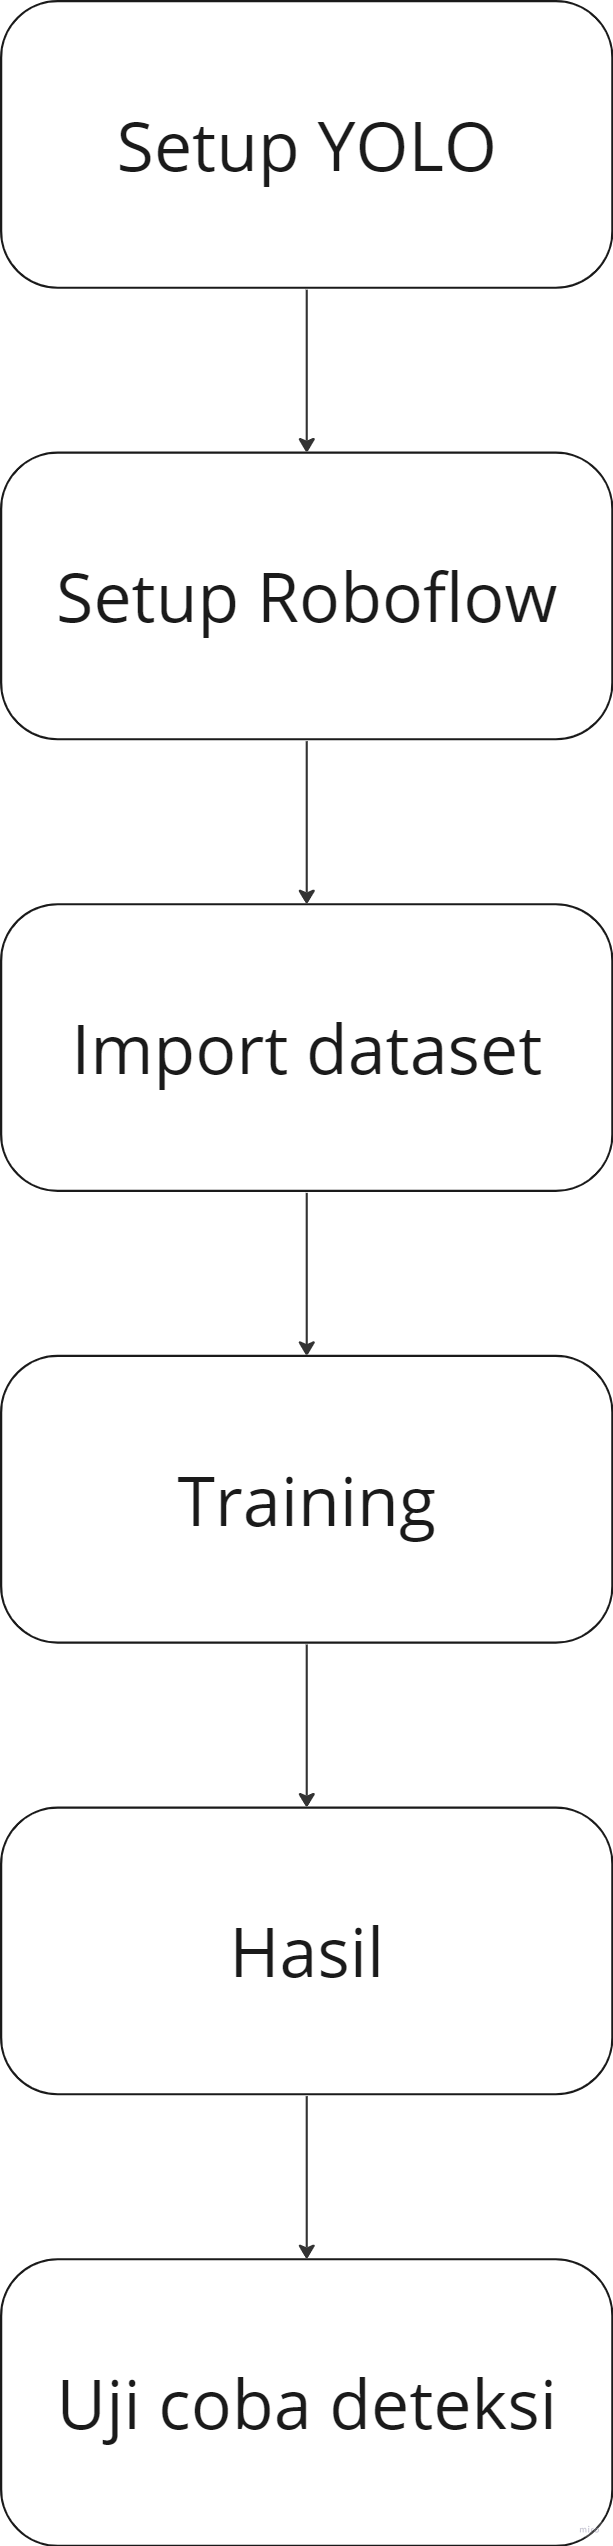
\includegraphics[scale=0.1]{gambar/bab3/deteksiyolo.png}
  \caption{Deteksi YOLOv9}
  \label{fig:deteksiyolo}
\end{figure}

\begin{algorithm}
  \caption{Training and Inference with YOLOv9 on a Custom Dataset}
  \begin{algorithmic}[1]
  \State Mount Google Drive for file access
  \State Check GPU availability using \texttt{nvidia-smi}
  \State Define the home directory and verify it with a print statement
  \State Clone YOLOv9 repository and navigate into it
  \State Install required libraries from the requirements file
  \State Install additional package, Roboflow
  
  \State Download model weights to the specified home directory weights folder
  \State Prepare the data directory within the home directory
  \State Download the dataset using Roboflow and configure it for YOLOv9
  
  \State Train the model using custom weights and hyperparameters
  \State Mount Google Drive if necessary
  \State Download the best model weights after training
  
  \State List training results including images and plots
  \State Display training result images using IPython display functionality
  
  \State Validate the custom model with specified parameters
  \State Perform detection using the trained model on validation images
  
  \State Display confusion matrix and a subset of detection result images
  \end{algorithmic}
\end{algorithm}

Pada program ini, pertama-tama dilakukan import library yang dibutuhkan. Selanjutnya, dilakukan setup YOLOv9 dengan melakukan clone YOLOv9 dari repository github yang kemudian dilakukan instalasi berdasarkan file requirement.txt agar YOLOv9 bisa bekerja. Selanjutnya, program melakukan intalasi Roboflow yang mana hal ini bertujuan agar program bisa melakukan import dari platform Roboflow karena dataset yang digunakan dianotasi pada platform tersebut. Didapatkan bobot YOLOv9 dari repository github yang telah diclone dan melakukan penyesuaian nilai jumlah kelas yang akan dideteksi sesuai dengan jumlah kelas yang ada.

Program kemudian akan melakukan import dataset dari Roboflow dimana dataset tersebut sudah dianotasi. Dilakukan proses training dengan mengatur beberapa parameter seperti ukuran batch, jumlah epoch, ukuran gambar. Ukuran batch diatur menjadi 8, jumlah epoch diatur menjadi 10, dan ukuran gambar diatur menjadi 640x640 piksel menyesuaikan dengan dataset yang telah dilakukan bounding box pada Roboflow. Setelah proses training, didapatkan nilai dari akurasi model tersebut. Kemudian dilakukan prediksi pada yang telah tersedia.
\cleardoublepage

% Bab 4 pengujian dan analisis
\chapter{PENGUJIAN DAN ANALISIS}
\label{chap:pengujiananalisis}

% Ubah bagian-bagian berikut dengan isi dari pengujian dan analisis

Pada bab ini akan dipaparkan mengenai beberapa hasil pengujian sesuai dengan telah dijelaskan pada metodologi. Hasil pengujian ini dilakukan guna untuk mendapatkan hasil klasifikasi dan deteksi yang optimal. Pelaksanaan metodologi serta hasil pengujian yang akan dipaparkan dalam bab ini diharapkan dapat memberikan pemahaman mengenai hasil dan pembahasan sehingga dapat ditarik kesimpulan dari Tugas Akhir yang telah dilaksanakan.


\section{Pengujian Klasifikasi Menggunakan CNN 2-Dimensi}
\label{sec:PengujianCNN2D}
Proses klasifikasi menggunakan CNN 2-Dimensi dilakukan sebanyak tiga kali percobaan. Pada setiap percobaan, dilakukan training dengan pengaturan CNN 2-Dimensi yang sama kecuali dalam satu hal. Setiap percobaan dilakukan dengan pembagian jumlah data berbeda-beda untuk training, valiation, dan testing. Dari hasil tersebut akan dilakukan variasi struktur CNN 2-Dimensi dengan pembagian dataset yang memiliki hasil yang baik. Hasil klasifikasi menggunakan CNN 2-Dimensi akan dibandingkan dengan hasil klasifikasi menggunakan Roboflow dan CNN 2-Dimensi pada percobaan yang lain. Pada pengujian CNN 2-Dimensi ini nantinya akan digunakan gambar yang sama dalam masing-masing eksperimen.

\subsection{Percobaan Pertama}
Pada percobaan pertama, data yang digunakan untuk training, validation, dan testing masing-masing sebanyak 70\%, 20\%, dan 10\%. Hasil klasifikasi menggunakan CNN 2-Dimensi pada percobaan pertama mendapatkan tingkat akurasi training sebesar 0.9918 dengan training loss sebesar 0.0235. Sementara itu, didapatkan tingkat akurasi validasi sebesar 1.0 dengan valiation loss sebesar 4.6915e-05. Berikut ini adalah grafik model accuracy dan model loss pada percobaan pertama yang dapat dilihat pada Gambar \ref{fig:trainres1}.

\begin{figure} [H] \centering
    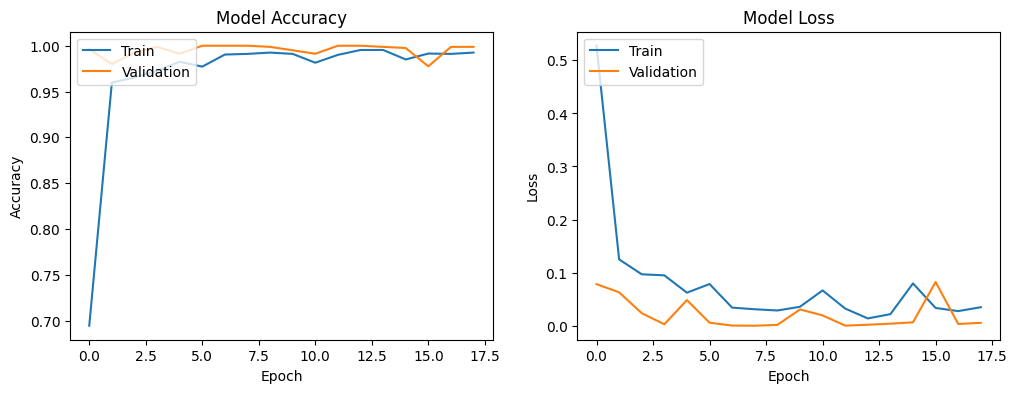
\includegraphics[scale=0.5]{gambar/bab4/trainres1.png}
    \caption{Grafik Akurasi dan Loss Model Percobaan Pertama}
    \label{fig:trainres1}
\end{figure}

Selain itu, didapatkan pula hasil confusion matrix dari data training, validation, dan testing pada percobaan pertama yang masing-masing dapat dilihat pada Gambar \ref{fig:tvcon1} dan \ref{fig:testcon1}. Dari hasil tersebut, dapat dilihat bahwa hasil klasifikasi menggunakan CNN 2-Dimensi pada percobaan pertama memiliki tingkat akurasi yang cukup tinggi. Hal ini didukung dengan nilai f1 score pada data training sebesar 0.98926264, validation sebesar 1.0, dan testing sebesar 0.99750614. Inference time yang didapatkan pada percobaan pertama untuk data training sebanyak 2804 data adalah 79 detik (283ms/step), untuk data validation sebanyak 800 data adalah 9 detik (117ms/step), dan untuk data testing sebanyak 400 data adalah 164 detik (4s/step).

\begin{figure} [H] \centering
    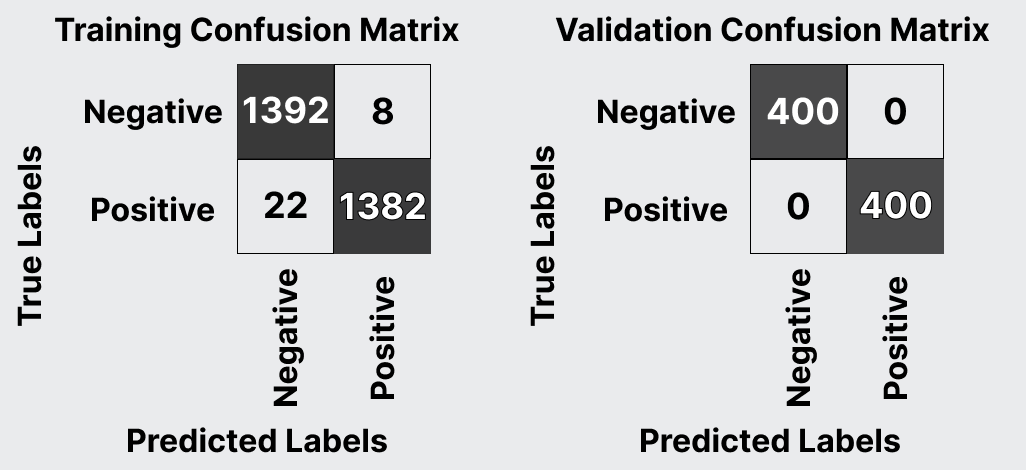
\includegraphics[scale=0.3]{gambar/bab4/tvcon1.png}
    \caption{Confussion Matrix Training dan Validasi Percobaan Pertama}
    \label{fig:tvcon1}
\end{figure}

\begin{figure} [H] \centering
    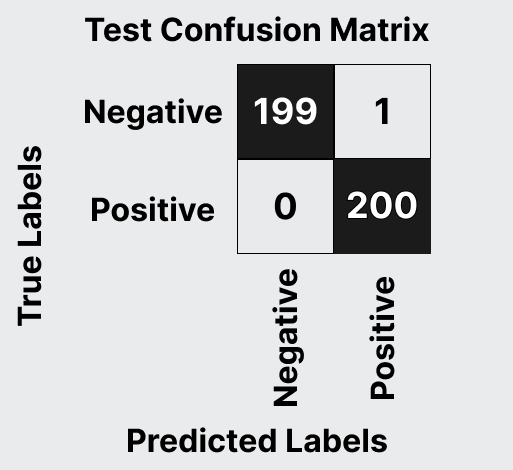
\includegraphics[scale=0.3]{gambar/bab4/testcon1.png}
    \caption{Confussion Matrix Testing Percobaan Pertama}
    \label{fig:testcon1}
\end{figure}

Hasil training yang cukup baik dari percobaan pertama dapat dilihat pula pada keberhasilannya dalam mengklasifikasikan gambar dengan tepat seperti yang dapat dilihat pada gambar berikut:

\begin{figure} [H] \centering
    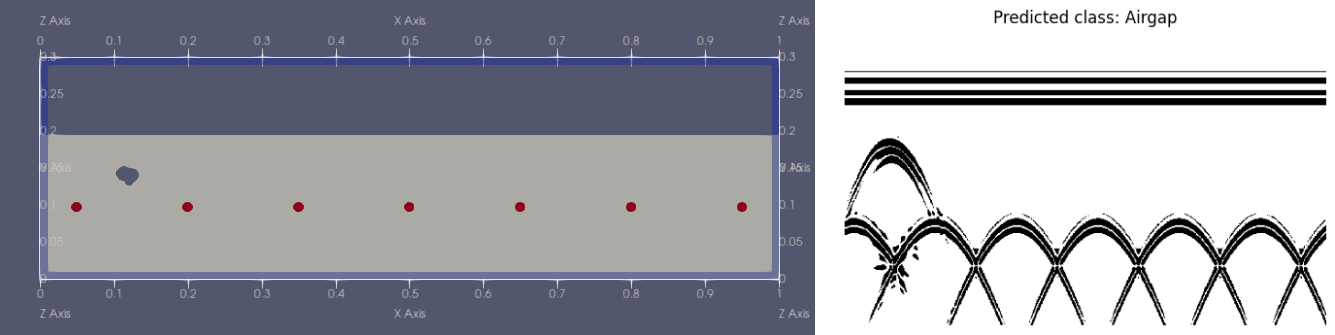
\includegraphics[scale=0.2]{gambar/bab4/Airgap 1999.png}
    \caption{Hasil Klasifikasi Percobaan Pertama 1}
\end{figure}

\begin{figure} [H] \centering
    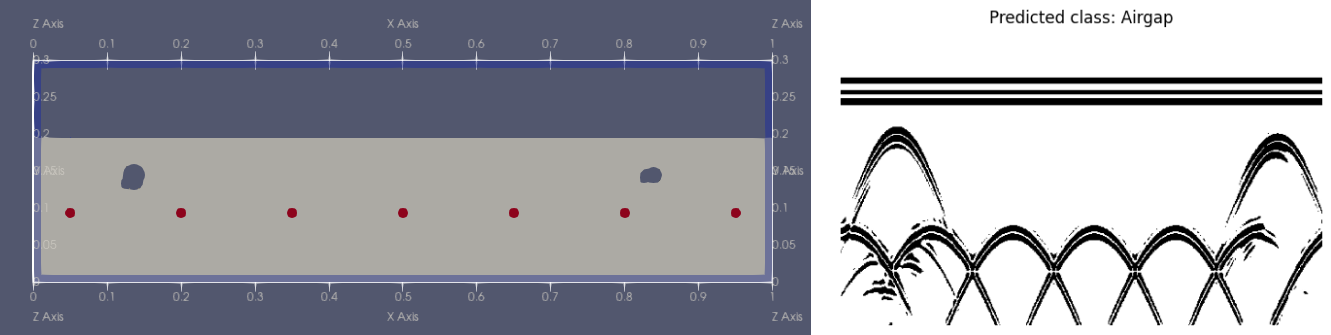
\includegraphics[scale=0.2]{gambar/bab4/Airgap 2000.png}
    \caption{Hasil Klasifikasi Percobaan Pertama 2}
\end{figure}

\begin{figure} [H] \centering
    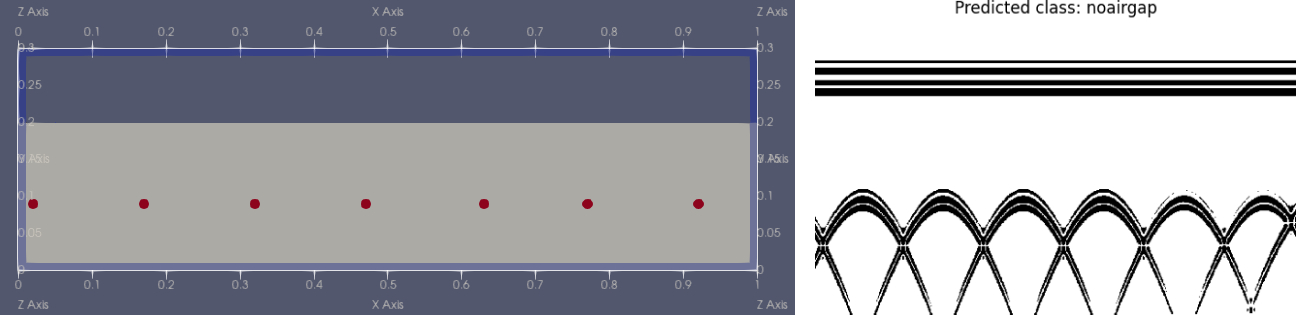
\includegraphics[scale=0.2]{gambar/bab4/Noarigap 1900.png}
    \caption{Hasil Klasifikasi Percobaan Pertama 3}
\end{figure}

\begin{figure} [H] \centering
    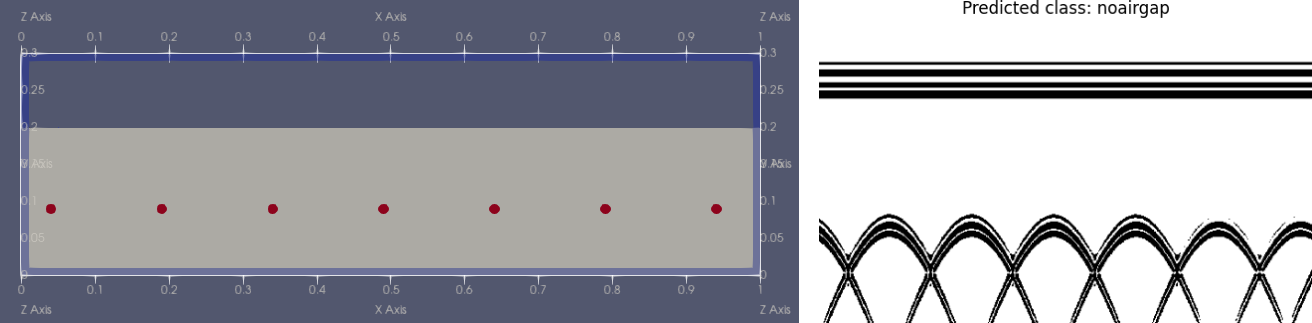
\includegraphics[scale=0.2]{gambar/bab4/Noairgap 2000.png}
    \caption{Hasil Klasifikasi Percobaan Pertama 4}
\end{figure}

\subsection{Percobaan Kedua}
Pada percobaan kedua, data yang digunakan untuk training, validation, dan testing masing-masing sebanyak 70\%, 15\%, dan 15\%. Hasil klasifikasi menggunakan CNN 2-Dimensi pada percobaan kedua mendapatkan tingkat akurasi training sebesar 0.9964 dengan training loss sebesar 0.0103. Sementara itu, didapatkan tingkat akurasi validasi sebesar 1.0 dengan valiation loss sebesar 2.0294e-04. Berikut ini adalah grafik model accuracy dan model loss pada percobaan kedua yang dapat dilihat pada Gambar \ref{fig:trainres2}.

\begin{figure} [H] \centering
    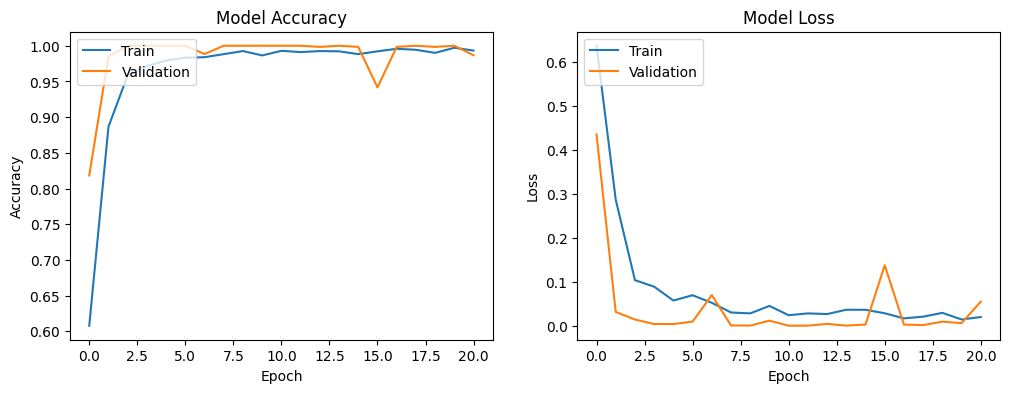
\includegraphics[scale=0.5]{gambar/bab4/trainres2.png}
    \caption{Grafik Akurasi dan Loss Model Percobaan Kedua}
    \label{fig:trainres2}
\end{figure}

Selain itu, didapatkan pula hasil confusion matrix dari data training, validation, dan testing pada percobaan kedua yang masing-masing dapat dilihat pada Gambar \ref{fig:tvcon2} dan \ref{fig:testcon2}. Dari hasil tersebut, dapat dilihat bahwa hasil klasifikasi menggunakan CNN 2-Dimensi pada percobaan kedua memiliki tingkat akurasi yang cukup tinggi. Hal ini didukung dengan nilai f1 score pada data training sebesar 0.99714893, validation sebesar 1.0, dan testing sebesar 1.0. Inference time yang didapatkan pada percobaan kedua untuk data training sebanyak 2800 data adalah 80 detik (285ms/step), untuk data validation sebanyak 600 data adalah 7 detik (115ms/step), dan untuk data testing sebanyak 600 data adalah 8 detik (128ms/step).

\begin{figure} [H] \centering
    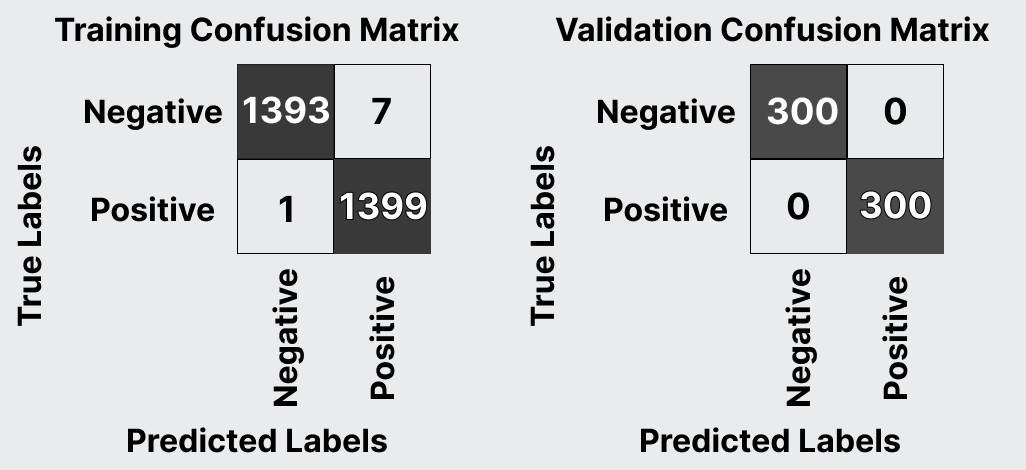
\includegraphics[scale=0.3]{gambar/bab4/tvcon2.png}
    \caption{Confussion Matrix Training dan Validasi Percobaan Kedua}
    \label{fig:tvcon2}
\end{figure}

\begin{figure} [H] \centering
    \includegraphics[scale=0.3]{gambar/bab4/testcon2.png}
    \caption{Confussion Matrix Testing Percobaan Kedua}
    \label{fig:testcon2}
\end{figure}

Hasil training yang cukup baik dari percobaan kedua dapat dilihat pula pada keberhasilannya dalam mengklasifikasikan gambar dengan tepat seperti yang dapat dilihat pada gambar berikut:

\begin{figure} [H] \centering
    \includegraphics[scale=0.2]{gambar/bab4/Airgap 19992.png}
    \caption{Hasil Klasifikasi Percobaan Kedua 1}
\end{figure}

\begin{figure} [H] \centering
    \includegraphics[scale=0.2]{gambar/bab4/Airgap 20002.png}
    \caption{Hasil Klasifikasi Percobaan Kedua 2}
\end{figure}

\begin{figure} [H] \centering
    \includegraphics[scale=0.2]{gambar/bab4/Noarigap 19002.png}
    \caption{Hasil Klasifikasi Percobaan Kedua 3}
\end{figure}

\begin{figure} [H] \centering
    \includegraphics[scale=0.2]{gambar/bab4/Noairgap 20002.png}
    \caption{Hasil Klasifikasi Percobaan Kedua 4}
\end{figure}

\subsection{Percobaan Ketiga}
Pada percobaan ketiga, data yang digunakan untuk training, validation, dan testing masing-masing sebanyak 60\%, 20\%, dan 20\%. Hasil klasifikasi menggunakan CNN 2-Dimensi pada percobaan ketiga mendapatkan tingkat akurasi training sebesar 0.9946 dengan training loss sebesar 0.0147. Sementara itu, didapatkan tingkat akurasi validasi sebesar 1.0 dengan valiation loss sebesar 1.1496e-04. Berikut ini adalah grafik model accuracy dan model loss pada percobaan ketiga yang dapat dilihat pada Gambar \ref{fig:trainres3}.

\begin{figure} [H] \centering
    \includegraphics[scale=0.5]{gambar/bab4/trainres3.png}
    \caption{Grafik Akurasi dan Loss Model Percobaan Ketiga}
    \label{fig:trainres3}
\end{figure}

Meskipun pada hasil training, model memiliki hasil yang baik, grafik hasil training menunjukan training yang tidak begitu baik dan mengindikasikan overfitting dengan adanya spiking. Tidak dipungkiri bahwa hal ini dapat terjadi karena pada salah satu kelas dataset yakni noairgap, kelas tersebut memiliki data yang hampir serupa satu sama lain. Selain itu, didapatkan pula hasil confusion matrix dari data training, validation, dan testing pada percobaan ketiga yang masing-masing dapat dilihat pada Gambar \ref{fig:tvcon3} dan \ref{fig:testcon3}. Dari hasil tersebut, dapat dilihat bahwa hasil klasifikasi menggunakan CNN 2-Dimensi pada percobaan ketiga memiliki tingkat akurasi yang baik. Meskipun pada confusion matriks data training dan valiasi masih menunjukkan kesalahan, namun pada data testing menunjukkan keakuratan yang baik. Hal ini didukung dengan nilai f1 score pada data training sebesar 0.99502486, validation sebesar 1.0, dan testing sebesar 1.0. Inference time yang didapatkan pada percobaan ketiga untuk data training sebanyak 2400 data adalah 72 detik (301ms/step), untuk data validation sebanyak 800 data adalah 9 detik (114ms/step), dan untuk data testing sebanyak 800 data adalah 115 detik (1s/step).

\begin{figure} [H] \centering
    \includegraphics[scale=0.3]{gambar/bab4/tvcon3.png}
    \caption{Confussion Matrix Training dan Validasi Percobaan Ketiga}
    \label{fig:tvcon3}
\end{figure}

\begin{figure} [H] \centering
    \includegraphics[scale=0.3]{gambar/bab4/testcon3.png}
    \caption{Confussion Matrix Testing Percobaan Ketiga}
    \label{fig:testcon3}
\end{figure}

Hasil training yang cukup baik dari percobaan ketiga dapat dilihat pula pada keberhasilannya dalam mengklasifikasikan gambar dengan tepat seperti yang dapat dilihat pada gambar berikut:

\begin{figure} [H] \centering
    \includegraphics[scale=0.2]{gambar/bab4/Airgap 19993.png}
    \caption{Hasil Klasifikasi Percobaan Ketiga 1}
\end{figure}

\begin{figure} [H] \centering
    \includegraphics[scale=0.2]{gambar/bab4/Airgap 20003.png}
    \caption{Hasil Klasifikasi Percobaan Ketiga 2}
\end{figure}

\begin{figure} [H] \centering
    \includegraphics[scale=0.2]{gambar/bab4/Noarigap 19003.png}
    \caption{Hasil Klasifikasi Percobaan Ketiga 3}
\end{figure}

\begin{figure} [H] \centering
    \includegraphics[scale=0.2]{gambar/bab4/Noairgap 20003.png}
    \caption{Hasil Klasifikasi Percobaan Ketiga 4}
\end{figure}

\subsection{Percobaan Keempat}
Pada percobaan keempat, data yang digunakan untuk training, validation, dan testing masing-masing sebanyak 70\%, 15\%, dan 15\%. Selain itu, ditambahkan variasi untuk kode CNN 2-Dimensi dengan menambahkan BatchNormalization setelah setiap layer Conv2D. Hasil klasifikasi menggunakan CNN 2-Dimensi pada percobaan keempat mendapatkan tingkat akurasi training sebesar 0.9621 dengan training loss sebesar 0.1670. Sementara itu, didapatkan tingkat akurasi validasi sebesar 0.9833 dengan valiation loss sebesar 0.1061. Berikut ini adalah grafik model accuracy dan model loss pada percobaan keempat yang dapat dilihat pada Gambar \ref{fig:trainres4}.

\begin{figure} [H] \centering
    \includegraphics[scale=0.5]{gambar/bab4/trainres4.png}
    \caption{Grafik Akurasi dan Loss Model Percobaan Keempat}
    \label{fig:trainres4}
\end{figure}

Berdasarkan grafik hasil training, meskipun hasil memiliki tingkat keakurasian yang baik, grafik menunjukkan perilaku yang tidak wajar dimana terjadi spiking yang tinggi. Hal ini dapat terjadi karena pada salah satu kelas dataset yakni noairgap, kelas tersebut memiliki data yang hampir serupa satu sama lain. Penyebab lain dapat bersumber dari perubahan struktur layer CNN 2-Dimensis yang digunakan. Selain itu, didapatkan pula hasil confusion matrix dari data training, validation, dan testing pada percobaan keempat yang masing-masing dapat dilihat pada Gambar \ref{fig:tvcon4} dan \ref{fig:testcon4}. Dari hasil tersebut, dapat dilihat bahwa hasil klasifikasi menggunakan CNN 2-Dimensi pada percobaan keempat memiliki tingkat akurasi sedang. Hal ini didukung dengan hasil confusion matrix pada data training, validasi, dan testing yang memiliki error yang lebih banyak dibandingkan dengan percobaan yang lain. Nilai f1 score yang didapatkan pada data training sebesar 0.961155, validation sebesar 0.98360646, dan testing sebesar 0.9803921. Inference time yang didapatkan pada percobaan keempat untuk data training sebanyak 2800 data adalah 79 detik (281ms/step), untuk data validation sebanyak 600 data adalah 10 detik (162ms/step), dan untuk data testing sebanyak 600 data adalah 130 detik (2s/step).

\begin{figure} [H] \centering
    \includegraphics[scale=0.3]{gambar/bab4/tvcon4.png}
    \caption{Confussion Matrix Training dan Validasi Percobaan Keempat}
    \label{fig:tvcon4}
\end{figure}

\begin{figure} [H] \centering
    \includegraphics[scale=0.3]{gambar/bab4/testcon4.png}
    \caption{Confussion Matrix Testing Percobaan Keempat}
    \label{fig:testcon4}
\end{figure}

Hasil training yang cukup baik dari percobaan keempat dapat dilihat pula pada keberhasilannya dalam mengklasifikasikan gambar dengan tepat seperti yang dapat dilihat pada gambar berikut:

\begin{figure} [H] \centering
    \includegraphics[scale=0.2]{gambar/bab4/Airgap 19994.png}
    \caption{Hasil Klasifikasi Percobaan Keempat 1}
\end{figure}

\begin{figure} [H] \centering
    \includegraphics[scale=0.2]{gambar/bab4/Airgap 20004.png}
    \caption{Hasil Klasifikasi Percobaan Keempat 2}
\end{figure}

\begin{figure} [H] \centering
    \includegraphics[scale=0.2]{gambar/bab4/Noarigap 19004.png}
    \caption{Hasil Klasifikasi Percobaan Keempat 3}
\end{figure}

\begin{figure} [H] \centering
    \includegraphics[scale=0.2]{gambar/bab4/Noairgap 20004.png}
    \caption{Hasil Klasifikasi Percobaan Keempat 4}
\end{figure}

\subsection{Percobaan Kelima}
Pada percobaan kelima, data yang digunakan untuk training, validation, dan testing masing-masing sebanyak 70\%, 15\%, dan 15\%. Pada percobaan ini, ditambahkan variasi untuk kode CNN 2-Dimensi dengan mengurangi jumlah layer Conv2D menjadi dua dan layer Dense menjadi 1. Layer Conv2D berawal dari 32 dan berakhir di 64 dengan MaxPooling dan BatchNormalization yang sama dengan percobaan keempat. Hasil klasifikasi menggunakan CNN 2-Dimensi pada percobaan kelima mendapatkan tingkat akurasi training sebesar 0.9154 dengan training loss sebesar 0.2236. Sementara itu, didapatkan tingkat akurasi validasi sebesar 0.9867 dengan valiation loss sebesar 0.0336. Berikut ini adalah grafik model accuracy dan model loss pada percobaan kelima yang dapat dilihat pada Gambar \ref{fig:trainres5}.

\begin{figure} [H] \centering
    \includegraphics[scale=0.5]{gambar/bab4/trainres5.png}
    \caption{Grafik Akurasi dan Loss Model Percobaan Kelima}
    \label{fig:trainres5}
\end{figure}

Berdasarkan grafik hasil training, meskipun hasil memiliki tingkat keakurasian yang lebih rendah dibandingkan percobaan sebelumnya, grafik menunjukkan perilaku yang tidak wajar dimana grafik menunjukan nilai yang tinggi kemudian rendah berulang kali. Hal ini dapat terjadi karena pada salah satu kelas dataset yakni noairgap, kelas tersebut memiliki data yang hampir serupa satu sama lain. Penyebab lain dapat bersumber dari perubahan struktur layer CNN 2-Dimensis yang digunakan. Selain itu, didapatkan pula hasil confusion matrix dari data training, validation, dan testing pada percobaan kelima yang masing-masing dapat dilihat pada Gambar \ref{fig:tvcon5} dan \ref{fig:testcon5}. Dari hasil tersebut, dapat dilihat bahwa hasil klasifikasi menggunakan CNN 2-Dimensi pada percobaan kelima terjadi penurunan dalam hal tingkat akurasi. Didapatkan nilai f1 score pada data training sebesar 0.92211217, validation sebesar 0.98684204, dan testing sebesar 0.98360646. Inference time yang didapatkan pada percobaan kelima untuk data training sebanyak 2800 data adalah 85 detik (304ms/step), untuk data validation sebanyak 600 data adalah 8 detik (125ms/step), dan untuk data testing sebanyak 600 data adalah 83 detik (1s/step).

\begin{figure} [H] \centering
    \includegraphics[scale=0.3]{gambar/bab4/tvcon5.png}
    \caption{Confussion Matrix Training dan Validasi Percobaan Kelima}
    \label{fig:tvcon5}
\end{figure}

\begin{figure} [H] \centering
    \includegraphics[scale=0.3]{gambar/bab4/testcon5.png}
    \caption{Confussion Matrix Testing Percobaan Kelima}
    \label{fig:testcon5}
\end{figure}

Hasil training yang cukup baik dari percobaan kelima dapat dilihat pula pada keberhasilannya dalam mengklasifikasikan gambar dengan tepat seperti yang dapat dilihat pada gambar berikut:

\begin{figure} [H] \centering
    \includegraphics[scale=0.2]{gambar/bab4/Airgap 19995.png}
    \caption{Hasil Klasifikasi Percobaan Kelima 1}
\end{figure}

\begin{figure} [H] \centering
    \includegraphics[scale=0.2]{gambar/bab4/Airgap 20005.png}
    \caption{Hasil Klasifikasi Percobaan Kelima 2}
\end{figure}

\begin{figure} [H] \centering
    \includegraphics[scale=0.2]{gambar/bab4/Noarigap 19005.png}
    \caption{Hasil Klasifikasi Percobaan Kelima 3}
\end{figure}

\begin{figure} [H] \centering
    \includegraphics[scale=0.2]{gambar/bab4/Noairgap 20005.png}
    \caption{Hasil Klasifikasi Percobaan Kelima 4}
\end{figure}

\subsection{Percobaan Keenam}
Pada percobaan keenam, data yang digunakan untuk training, validation, dan testing masing-masing sebanyak 70\%, 15\%, dan 15\%. Pada percobaan ini, ditambahkan variasi untuk kode CNN 2-Dimensi dengan menjadikan struktur CNN 2-Dimensi hanya memiliki 3 layer Conv2D tanpa BatchNormalization, masih memiliki MaxPooling yang sama namun layer Conv2D memiliki parameter tambahan yakni padding yang nilainya diatur menjadi 'same' dengan layer Conv2D bermula dari 32 dan berakhir pada 128. Selain itu, ditambahkan dropout layer senilai 0.25 sebelum memasuki flatten layer dan ditambahkan 1 Dense layer setelahnya. Hasil klasifikasi menggunakan CNN 2-Dimensi pada percobaan keenam mendapatkan tingkat akurasi training sebesar 0.9993 dengan training loss sebesar 0.0028. Sementara itu, didapatkan tingkat akurasi validasi sebesar 1.0 dengan valiation loss sebesar 4.2127e-06. Berikut ini adalah grafik model accuracy dan model loss pada percobaan keenam yang dapat dilihat pada Gambar \ref{fig:trainres6}.

\begin{figure} [H] \centering
    \includegraphics[scale=0.5]{gambar/bab4/trainres6.png}
    \caption{Grafik Akurasi dan Loss Model Percobaan Keenam}
    \label{fig:trainres6}
\end{figure}

Berdasarkan grafik hasil training, meskipun hasil memiliki tingkat keakurasian yang perlahan-lahan membaik dibandingkan percobaan sebelumnya, grafik menunjukkan perilaku yang tidak wajar dimana grafik menunjukan spiking yang tinggi. Hal ini dapat terjadi karena pada salah satu kelas dataset yakni noairgap, kelas tersebut memiliki data yang hampir serupa satu sama lain. Selain itu, didapatkan pula hasil confusion matrix dari data training, validation, dan testing pada percobaan keenam yang masing-masing dapat dilihat pada Gambar \ref{fig:tvcon6} dan \ref{fig:testcon6}. Dari hasil tersebut, dapat dilihat bahwa hasil klasifikasi menggunakan CNN 2-Dimensi pada percobaan keenam memiliki tingkat akurasi yang cukup tinggi. Hal ini didukung dengan nilai f1 score pada data training sebesar 0.9985734, validation sebesar 1.0, dan testing sebesar 1.0. Inference time yang didapatkan pada percobaan keenam untuk data training sebanyak 2800 data adalah 76 detik (269ms/step), untuk data validation sebanyak 600 data adalah 7 detik (119ms/step), dan untuk data testing sebanyak 600 data adalah 97 detik (2s/step).

\begin{figure} [H] \centering
    \includegraphics[scale=0.3]{gambar/bab4/tvcon6.png}
    \caption{Confussion Matrix Training dan Validasi Percobaan Keenam}
    \label{fig:tvcon6}
\end{figure}

\begin{figure} [H] \centering
    \includegraphics[scale=0.3]{gambar/bab4/testcon6.png}
    \caption{Confussion Matrix Testing Percobaan Keenam}
    \label{fig:testcon6}
\end{figure}

Hasil training yang cukup baik dari percobaan keenam dapat dilihat pula pada keberhasilannya dalam mengklasifikasikan gambar dengan tepat seperti yang dapat dilihat pada gambar berikut:

\begin{figure} [H] \centering
    \includegraphics[scale=0.2]{gambar/bab4/Airgap 19996.png}
    \caption{Hasil Klasifikasi Percobaan Keenam 1}
\end{figure}

\begin{figure} [H] \centering
    \includegraphics[scale=0.2]{gambar/bab4/Airgap 20006.png}
    \caption{Hasil Klasifikasi Percobaan Keenam 2}
\end{figure}

\begin{figure} [H] \centering
    \includegraphics[scale=0.2]{gambar/bab4/Noarigap 19006.png}
    \caption{Hasil Klasifikasi Percobaan Keenam 3}
\end{figure}

\begin{figure} [H] \centering
    \includegraphics[scale=0.2]{gambar/bab4/Noairgap 20006.png}
    \caption{Hasil Klasifikasi Percobaan Keenam 4}
\end{figure}

Dari semua percobaan diatas, dapat diketahui bahwa hasil terbaik didapatkan pada percobaan kedua. Meskipun semua percobaan memiliki hasil klasifikasi yang baik, percobaan kedua memiliki hasil metrics yang lebih baik dibandingkan dengan percobaan lainnya.

\subsection{Percobaan Ketujuh}
Pada percobaan Ketujuh, data yang digunakan untuk training, validation, dan testing masing-masing sebanyak 70\%, 15\%, dan 15\%. Pada percobaan ini, ditambahkan variasi untuk kode CNN 2-Dimensi dengan menjadikan struktur CNN 2-Dimensi memiliki 6 layer Conv2D dengan masih memiliki MaxPooling yang sama namun hanya pada empat layer pertama. Selain itu, model ini tidak menggunakan dropout layer serta sebelum memasuki flatten layer dan ditambahkan 1 Dense layer setelahnya. Hasil klasifikasi menggunakan CNN 2-Dimensi pada percobaan ketujuh mendapatkan tingkat akurasi training sebesar 0.9979 dengan training loss sebesar 0.0060. Sementara itu, didapatkan tingkat akurasi validasi sebesar 1.0 dengan valiation loss sebesar 1.7544e-04. Berikut ini adalah grafik model accuracy dan model loss pada percobaan ketujuh yang dapat dilihat pada Gambar \ref{fig:trainres7}.

\begin{figure} [H] \centering
    \includegraphics[scale=0.5]{gambar/bab4/trainres7.png}
    \caption{Grafik Akurasi dan Loss Model Percobaan Ketujuh}
    \label{fig:trainres7}
\end{figure}

Berdasarkan grafik hasil training, grafik menunjukkan perilaku yang tidak wajar dimana grafik menunjukan spiking yang tinggi. Hal ini dapat terjadi karena pada salah satu kelas dataset yakni noairgap, kelas tersebut memiliki data yang hampir serupa satu sama lain. Selain itu, didapatkan pula hasil confusion matrix dari data training, validation, dan testing pada percobaan ketujuh yang masing-masing dapat dilihat pada Gambar \ref{fig:tvcon7} dan \ref{fig:testcon7}. Dari hasil tersebut, dapat dilihat bahwa hasil klasifikasi menggunakan CNN 2-Dimensi pada percobaan ketujuh memiliki tingkat akurasi yang tinggi. Hal ini didukung dengan nilai f1 score pada data training sebesar 0.9985734, validation sebesar 1.0, dan testing sebesar 1.0. Inference time yang didapatkan pada percobaan ketujuh untuk data training sebanyak 2800 data adalah 76 detik (269ms/step), untuk data validation sebanyak 600 data adalah 6 detik (107ms/step), dan untuk data testing sebanyak 600 data adalah 81 detik (1s/step).

\begin{figure} [H] \centering
    \includegraphics[scale=0.3]{gambar/bab4/tvcon7.png}
    \caption{Confussion Matrix Training dan Validasi Percobaan Ketujuh}
    \label{fig:tvcon7}
\end{figure}

\begin{figure} [H] \centering
    \includegraphics[scale=0.3]{gambar/bab4/testcon7.png}
    \caption{Confussion Matrix Testing Percobaan Ketujuh}
    \label{fig:testcon7}
\end{figure}

Hasil training yang cukup baik dari percobaan ketujuh dapat dilihat pula pada keberhasilannya dalam mengklasifikasikan gambar dengan tepat seperti yang dapat dilihat pada gambar berikut:

\begin{figure} [H] \centering
    \includegraphics[scale=0.2]{gambar/bab4/Airgap 19997.png}
    \caption{Hasil Klasifikasi Percobaan Ketujuh 1}
\end{figure}

\begin{figure} [H] \centering
    \includegraphics[scale=0.2]{gambar/bab4/Airgap 20007.png}
    \caption{Hasil Klasifikasi Percobaan Ketujuh 2}
\end{figure}

\begin{figure} [H] \centering
    \includegraphics[scale=0.2]{gambar/bab4/Noarigap 19007.png}
    \caption{Hasil Klasifikasi Percobaan Ketujuh 3}
\end{figure}

\begin{figure} [H] \centering
    \includegraphics[scale=0.2]{gambar/bab4/Noairgap 20007.png}
    \caption{Hasil Klasifikasi Percobaan Ketujuh 4}
\end{figure}

Dari semua percobaan diatas, dapat diketahui bahwa hasil terbaik didapatkan pada percobaan kedua. Meskipun semua percobaan memiliki hasil klasifikasi yang baik, percobaan kedua memiliki hasil metrics yang lebih baik dibandingkan dengan percobaan lainnya. Hal tersebut dapat terlihat dari tabel \ref{tab:perbaningancnn} berikut.

\begin{table}[H]
    \centering
    \begin{tabular}{|c|c|c|c|c|c|c|}
        \hline
        \textbf{Percobaan ke} & \multicolumn{3}{c|}{\textbf{F1 Score}} & \multicolumn{3}{c|}{\textbf{Inference Time / step}}                                                \\ \cline{2-7}
                              & Training                               & Validation                                          & Testing    & Training & Validation & Testing \\ \hline
        1                     & 0.98926264                             & 1.0                                                 & 0.99750614 & 283ms    & 117ms      & 4s      \\ \hline
        2                     & 0.99714893                             & 1.0                                                 & 1.0        & 285ms    & 115ms      & 125ms   \\ \hline
        3                     & 0.99502486                             & 1.0                                                 & 1.0        & 301ms    & 114ms      & 1s      \\ \hline
        4                     & 0.961155                               & 0.98360646                                          & 0.9803921  & 281ms    & 162ms      & 2s      \\ \hline
        5                     & 0.92211217                             & 0.98684204                                          & 0.98360646 & 304ms    & 125ms      & 1s      \\ \hline
        6                     & 0.9985734                              & 1.0                                                 & 1.0        & 269ms    & 119ms      & 2s      \\ \hline
        7                     & 0.9985734                              & 1.0                                                 & 1.0        & 269ms    & 107ms      & 1s      \\ \hline
    \end{tabular}
    \caption{Tabel Perbandingan Hasil F1 Score dan Inference Time}
    \label{tab:perbaningancnn}
\end{table}

Berdasarkan tabel \ref{tab:perbaningancnn} diatas, dapat dilihat bahwa semua percobaan memiliki hasil F1 score dan inference time yang relatif sama. Akan tetapi, pada percobaan kedua, dihasilkan inference time yang paling cepat pada data testing dibandingkan dengan percobaan lainnya dengan selisih yang cukup besar. Oleh karena itu, percobaan kedua dipilih sebagai model terbaik untuk klasifikasi menggunakan CNN 2D.

\section{Pengujian Klasifikasi Roboflow}
\label{sec:PengujianRoboflow}
Proses klasifikasi menggunakan Roboflow hanya dilakukan satu kali dan hasil yang didapatkan akan dibandingkan dengan hasil klasifikasi menggunakan CNN 2-Dimensi. Hasil klasifikasi menggunakan Roboflow mendapatkan tingkat akurasi validasi sebesar 98.6\%. Selain itu, klasifikasi menggunakan juga menghasilkan grafik training loss dan valiation accuracy serta confusion matrix yang masing-masing dapat dilihat pada Gambar \ref{fig:roboflow} dan Gambar \ref{fig:confusionrobo}.

\begin{minipage}{\linewidth}
    \begin{figure} [H]
        \centering
        \includegraphics[scale=0.3]{gambar/bab4/roboflow.png}
        \caption{Hasil Training Loss dan Validation Accuracy Roboflow}
        \label{fig:roboflow}
    \end{figure}
\end{minipage}

\begin{minipage}{\linewidth}
    \begin{figure} [H]
        \centering
        \includegraphics[scale=1]{gambar/bab4/confusion.png}
        \caption{Confussion Matrix Roboflow}
        \label{fig:confusionrobo}
    \end{figure}
\end{minipage}

Dari hasil diatas, dapat didapatkan bahwa hasil klasifikasi menggunakan Roboflow memiliki tingkat akurasi yang cukup baik. Namun, hasil klasifikasi menggunakan Roboflow tidak dapat dijadikan sebagai acuan karena hanya dilakukan satu kali. Oleh karena itu, hasil klasifikasi menggunakan Roboflow akan dibandingkan dengan hasil klasifikasi menggunakan CNN 2-Dimensi serta akan diuji lagi melalui deteksi YOLOv9. Berikut ini merupakan hasil klasifikasi menggunakan Roboflow yang dapat dilihat pada gambar berikut:

\begin{figure} [H] \centering
    \includegraphics[scale=0.2]{gambar/bab4/robo1.png}
    \caption{Hasil Klasifikai Roboflow 1}
\end{figure}

\begin{figure} [H] \centering
    \includegraphics[scale=0.2]{gambar/bab4/robo2.png}
    \caption{Hasil Klasifikai Roboflow 2}
\end{figure}

\begin{figure} [H] \centering
    \includegraphics[scale=0.2]{gambar/bab4/robo3.png}
    \caption{Hasil Klasifikai Roboflow 3}
\end{figure}

\begin{figure} [H] \centering
    \includegraphics[scale=0.2]{gambar/bab4/robo4.png}
    \caption{Hasil Klasifikai Roboflow 4}
\end{figure}

\begin{figure} [H] \centering
    \includegraphics[scale=0.2]{gambar/bab4/robon.png}
    \caption{Hasil Klasifikai Roboflow 5}
\end{figure}

\section{Pengujian Deteksi YOLOv9}
\label{sec:PengujianYOLOv9}
Proses deteksi menggunakan YOLOv9 dilakukan sebanyak satu kali percobaan. Hasil klasifikasi menggunakan CNN 2-Dimensi dan Roboflow, nantinya akan dideteksi keberadaan rongga udaranya menggunakan YOLOv9 sehingga keberlangsungan pengujian deteksi menggunakan YOLOv9 sangat penting. Training YOLOv9 dilakukan dengan menggunakan dateset yang dilabeli melalui Roboflow. Dataset yang ada, dilakukan training dengan 10 epochs dan 8 batch. Dari hasil training, didapatkan hasil akurasi sebesar 0.979. Hasil metrics lainnya dapat dilihat pada gambar \ref{fig:metrics}. Selain itu, didapatkan pula hasil confusion matrix dari data training pada Gambar \ref{fig:conyolotrain}. Dari hasil tersebut, dapat dilihat bahwa hasil deteksi menggunakan YOLOv9 memiliki tingkat akurasi yang cukup tinggi.

\begin{figure} [H] \centering
    \includegraphics[scale=0.5]{gambar/bab4/metrics.png}
    \caption{Metrics YOLOv9}
    \label{fig:metrics}
\end{figure}

\begin{figure} [H] \centering
    \includegraphics[scale=0.1]{gambar/bab4/conyolotrain.png}
    \caption{Confussion Matrix YOLOv9}
    \label{fig:conyolotrain}
\end{figure}

Hasil confusion matrix diatas dapat terbentuk karena pada training YOLOv9 ini hanya digunakan satu kelas yakni kelas airgap atau rongga udara. Hal ini dilakukan karena pada penggunaan YOLOv9 ditunjukkan untuk mendeteksi satu objek saja yakni rongga udara pada sinyal B-Scan gprMax. Keakurasian YOLOv9 tersebut dapat dilihat dari hasil pengujian berikut dimana YOLOv9 mampu mendeteksi rongga udara pada sinyal B-Scan gprMax dengan baik. Berikut ini adalah contoh hasil deteksi menggunakan YOLOv9 yang dapat dilihat pada gambar berikut:

\begin{figure} [H] \centering
    \includegraphics[scale=0.2]{gambar/bab4/yolo1.png}
    \caption{Hasil Deteksi YOLOv9 1}
\end{figure}

\begin{figure} [H] \centering
    \includegraphics[scale=0.2]{gambar/bab4/yolo2.png}
    \caption{Hasil Deteksi YOLOv9 2}
\end{figure}

\begin{figure} [H] \centering
    \includegraphics[scale=0.2]{gambar/bab4/yolo3.png}
    \caption{Hasil Deteksi YOLOv9 3}
\end{figure}

\begin{figure} [H] \centering
    \includegraphics[scale=0.2]{gambar/bab4/yolo4.png}
    \caption{Hasil Deteksi YOLOv9 4}
\end{figure}
\cleardoublepage

% Bab 5 penutup
\chapter{PENUTUP}
\label{chap:penutup}

Pada bab ini akan dipaparkan kesimpulan dari hasil pengujian yang akan menjawab dari permasalahan yang diangkat dari pelaksanaan tugas akhir ini. Pada bab ini juga diapaprkan saran mengenai hal yang dapat dilakukan untuk mengembangkan penelitian kedepannya.

% Ubah bagian-bagian berikut dengan isi dari penutup

\section{Kesimpulan}
\label{sec:kesimpulan}

Berdasarkan hasil pengujian yang dilakukan selama pelaksanaan tugas akhir ini adalah sebagai berikut:

\begin{enumerate}[nolistsep]
  \item Model CNN 2D memiliki akurasi yang baik bila dataset dibagi menjadi 70\% training, 15\% validasi, dan 15\% testing
  \item Model dengan akurasi tertinggi didapatkan pada percobaan kedua dengan nilai akurasi sebesar 0.9964 dan training loss sebesar 0.0103. Didapatkan pula nilai f1 score sebesar 0.99714893
  \item Hasil training cenderung memicu lonjakan baik kecil maupun besar yang disebabkan oleh dataset yang digunakan dimana dataset sinyal B-Scan dari simulasi gprMax pada kelas tanpa rongga udara memiliki bentuk yang hampir serupa dengan sedikit variasi
  \item Hasil klasifikasi dengan Roboflow memiliki hasil yang tidak kalah baik dibandingkan dengan CNN 2D
  \item Pendeteksian dengan YOLOv9 memiliki akurasi yang baik sebesar 0.979 dapat mendeteksi rongga udara dengan baik
\end{enumerate}

\section{Saran}
\label{chap:saran}

Berdasarkan hasil yang diperoleh dari penelitian ini maka saran yang dapat dipertimbangkan untuk pengembangan lebih lanjut adalah sebagai berikut:

\begin{enumerate}[nolistsep]
  \item Memperbanyak variasi dari kedua kelas dataset yang digunakan
  \item Mencoba model CNN 2D yang lebih beragam untuk mengetahui model yang lebih efektif dan efisien
\end{enumerate}

\cleardoublepage

\chapter*{DAFTAR PUSTAKA}
\addcontentsline{toc}{chapter}{DAFTAR PUSTAKA}
\renewcommand\refname{}
\vspace{2ex}
\renewcommand{\bibname}{}
\begingroup
\def\chapter*#1{}
\printbibliography
\endgroup
\cleardoublepage

\chapter*{LAMPIRAN}

\section*{Kode Program}

\subsection*{Program Contoh Data Input gprMax}
\begin{lstlisting}[
    caption={Contoh File Input gprMax},
    label={lst:gprMaxinput}
]
#title: B-scan from rebar in concrete

#domain: 1.0 0.3 0.001
#dx_dy_dz: 0.001 0.001 0.001
#time_window: 3e-9

#material: 7.0 0.0 1.0 0.0 concrete
#material: 12.0 1.0e6 1.0 0.0 steel

#waveform: ricker 1 4.5e9 my_ricker
#src_steps: 0.001 0 0
#rx_steps: 0.001 0 0
#box: 0.0 0.0 0.0 1.0 0.203 0.001 concrete
#hertzian_dipole: z 0.010 0.203 0 my_ricker
#rx: 0.050 0.203 0
#cylinder: 0.154 0.092 0.0 0.154 0.092 0.001 0.007 steel
#cylinder: 0.304 0.092 0.0 0.304 0.092 0.001 0.007 steel
#cylinder: 0.454 0.092 0.0 0.454 0.092 0.001 0.007 steel
#cylinder: 0.604 0.092 0.0 0.604 0.092 0.001 0.007 steel
#cylinder: 0.754 0.092 0.0 0.754 0.092 0.001 0.007 steel
#cylinder: 0.904 0.092 0.0 0.904 0.092 0.001 0.007 steel
#cylinder: 0.054 0.092 0.0 0.054 0.092 0.001 0.007 steel
#cylinder: 0.416 0.129 0.0 0.416 0.129 0.001 0.013 free_space
#cylinder: 0.425 0.121 0.0 0.425 0.121 0.001 0.009 free_space
#cylinder: 0.416 0.122 0.0 0.416 0.122 0.001 0.015 free_space
#cylinder: 0.505 0.120 0.0 0.505 0.120 0.001 0.015 free_space
#cylinder: 0.499 0.117 0.0 0.499 0.117 0.001 0.010 free_space
#cylinder: 0.499 0.110 0.0 0.499 0.110 0.001 0.014 free_space
#cylinder: 0.495 0.116 0.0 0.495 0.116 0.001 0.011 free_space
#cylinder: 0.503 0.120 0.0 0.503 0.120 0.001 0.007 free_space
\end{lstlisting}

\subsection*{Program Generate File Input gprMax}
\begin{lstlisting}[
    language=Python,
    caption={Program untuk Menghasilkan File Input gprMax},
    label={lst:airauto}
]
import os
import random

def generate_airgap_cylinders(file, box_height):
    # Define bounds for airgap cylinder placement
    x_min, x_max = 0.05, 0.95
    y_min, y_max = 0.090, box_height - 0.05  # Adjusted Y bounds to ensure cylinders are within the concrete slab
    
    airgap_count = random.randint(1, 2)  # Generate 1 or 2 airgaps per file
    for _ in range(airgap_count):
        # Each airgap formed by 3 to 5 cylinders
        cylinder_count = random.randint(3, 5)
        
        # Initial positions for the first cylinder in an airgap
        x_position = random.uniform(x_min, x_max)
        y_position = random.uniform(y_min, y_max)

        for _ in range(cylinder_count):
            radius = random.uniform(0.010, 0.035) / 2  # Radius between 0.010m and 0.035m
            # Write cylinder, then adjust positions for the next one
            file.write(f"#cylinder: {x_position:.3f} {y_position:.3f} 0.0 {x_position:.3f} {y_position:.3f} 0.001 {radius:.3f} free_space\n")
            
            # Tighten adjustments for X and Y to encourage collisions
            x_adjust = random.uniform(-0.010, 0.010)
            y_adjust = random.uniform(-0.010, 0.010)
            
            # Update positions ensuring they remain within defined bounds
            x_position = min(max(x_position + x_adjust, x_min), x_max)
            y_position = min(max(y_position + y_adjust, y_min), y_max)

def generate_gprMax_files():
    base_content = """#title: B-scan from rebar in concrete

#domain: 1.0 0.3 0.001
#dx_dy_dz: 0.001 0.001 0.001
#time_window: 3e-9

#material: 7.0 0.0 1.0 0.0 concrete
#material: 12.0 1.0e6 1.0 0.0 steel

#waveform: ricker 1 4.5e9 my_ricker
#src_steps: 0.001 0 0
#rx_steps: 0.001 0 0
"""

    parent_folder = "airgap"
    os.makedirs(parent_folder, exist_ok=True)

    box_height_start = 0.190
    box_height_end = 0.210
    total_files = 2000  # Adjust total files generated to 2000

    for file_number in range(1, total_files + 1):
        box_height = random.uniform(box_height_start, box_height_end)
        folder_name = os.path.join(parent_folder, str(file_number))
        os.makedirs(folder_name, exist_ok=True)
        filename = os.path.join(folder_name, f"data{file_number}.in")

        with open(filename, "w") as file:
            file.write(base_content)
            file.write(f"#box: 0.0 0.0 0.0 1.0 {box_height:.3f} 0.001 concrete\n")
            file.write(f"#hertzian_dipole: z 0.010 {box_height:.3f} 0 my_ricker\n")
            file.write(f"#rx: 0.050 {box_height:.3f} 0\n")

            # Generate steel cylinders with a common Y position
            common_y_position = random.uniform(0.090, 0.110)  # Fixed Y position for steel cylinders within the range
            for position in [0.050, 0.200, 0.350, 0.500, 0.650, 0.800, 0.950]:
                new_x = (position + (file_number * 0.001)) % 1.0
                file.write(f"#cylinder: {new_x:.3f} {common_y_position:.3f} 0.0 {new_x:.3f} {common_y_position:.3f} 0.001 0.007 steel\n")

            # Generate abstract airgap shapes with tightened X and Y adjustments
            generate_airgap_cylinders(file, box_height)

            print(f"Generated file: {folder_name}/data{file_number}.in")

generate_gprMax_files()

\end{lstlisting}

\subsection*{Program Setup GPU}
\begin{lstlisting}[
    language=,
    caption={Program Setup GPU},
    label={lst:setupgpu}
]
#!/bin/bash

# Creating Miniconda directory
echo "Creating Miniconda directory..."
mkdir -p ~/miniconda3

# Downloading Miniconda installer
echo "Downloading Miniconda installer..."
wget https://repo.anaconda.com/miniconda/Miniconda3-latest-Linux-x86_64.sh -O ~/miniconda3/miniconda.sh

# Installing Miniconda
echo "Installing Miniconda..."
bash ~/miniconda3/miniconda.sh -b -u -p ~/miniconda3

# Removing the installer to save space
echo "Removing Miniconda installer..."
rm -rf ~/miniconda3/miniconda.sh

# Initializing Conda for bash
echo "Initializing Conda for bash..."
~/miniconda3/bin/conda init bash

source ./.bashrc

# Updating Conda
echo "Updating Conda..."
conda update conda -y

# Installing Git
echo "Installing Git..."
conda install git -y

# Cloning the gprMax repository
echo "Cloning gprMax repository..."
git clone https://github.com/MaulanaGilang/gprMax.git

# Changing directory to gprMax
echo "Changing directory to gprMax..."
cd gprMax

# Creating Conda environment from file
echo "Creating Conda environment from conda_env.yml..."
conda env create -f conda_env.yml

# Activating the gprMax environment
echo "Activating gprMax environment..."
conda activate gprMax

# Building gprMax
echo "Building gprMax..."
python setup.py build

# Installing gprMax
echo "Installing gprMax..."
python setup.py install

# Installing PyCUDA
echo "Installing PyCUDA..."
pip install pycuda

echo "Setup complete. gprMax is ready to use."
\end{lstlisting}

\subsection*{Program Otomatiasi Generate Data Melalui gprMax dengan GPU}
\begin{lstlisting}[
    language=Python,
    caption={Program Otomatiasi Generate Data gprMax dengan GPU},
    label={lst:autogprmax}
]
import argparse
import os
import subprocess
from shutil import move
import re
import matplotlib.pyplot as plt
from tools.plot_Bscan import get_output_data, mpl_plot
from PIL import Image

def natural_keys(text):
    """Helper function for natural sorting (sorts text with embedded numbers correctly)."""
    return [int(c) if c.isdigit() else c for c in re.split('(\d+)', text)]

def list_in_files_recursive(directory):
    """List all .in files recursively in the given directory."""
    in_files = {}
    for root, dirs, files in os.walk(directory):
        for f in files:
            if f.endswith('.in'):
                key = os.path.splitext(f)[0]
                in_files[key] = os.path.join(root, f)
    return in_files

def run_gprMax(file_path, n, use_gpu):
    """Run gprMax command on a file."""
    gpu_flag = '-gpu' if use_gpu else ''
    command = f'python -m gprMax {file_path} -n {n} {gpu_flag}'
    print("Running command: ", command)
    subprocess.run(command, shell=True, check=True)

def merge_output_files(directory, file_without_ext):
    """Merge output files in the directory based on the .in filename and delete the original .out files."""
    subprocess.run(f'python -m tools.outputfiles_merge {directory}/{file_without_ext}', shell=True, check=True)
    
    # New code to delete original .out files
    pattern = f'^{file_without_ext}\d+\.out$'
    for f in os.listdir(directory):
        if re.match(pattern, f):
            os.remove(os.path.join(directory, f))

def ensure_directory_exists(directory):
    """Ensure the specified directory exists, create if it doesn't."""
    if not os.path.exists(directory):
        os.makedirs(directory)

def move_output_file(source_path, dest_directory):
    """Move the file to the specified output directory, creating the directory if necessary."""
    ensure_directory_exists(dest_directory)
    dest_path = os.path.join(dest_directory, os.path.basename(source_path))
    move(source_path, dest_path)

    return dest_path

def process_file(file_path, rxnumber, rxcomponent, non_greyscale_dir, greyscale_dir):
    """Generate plots for a .out file, save color and cropped images (without converting to grayscale)."""
    outputdata, dt = get_output_data(file_path, rxnumber, rxcomponent)
    plt_figure = mpl_plot(file_path, outputdata, dt, rxnumber, rxcomponent)
    plt_figure.axis('off')

    savefile = os.path.splitext(os.path.basename(file_path))[0]
    image_path_with_colorbar = os.path.join(non_greyscale_dir, savefile + '.jpg')
    cropped_image_path = os.path.join(greyscale_dir, savefile + '_cropped.jpg')  # Renamed variable for clarity

    plt_figure.savefig(image_path_with_colorbar, dpi=150, format='JPEG', bbox_inches='tight', pad_inches=0.1)
    plt.close()

    color_bar_width = 300  # Adjusted to 300 pixels as per requirement
    left_crop = 20  # Left side crop
    bottom_crop = 20  # Bottom side crop adjustment

    image = Image.open(image_path_with_colorbar)
    cropped_image = image.crop((left_crop, 0, image.width - color_bar_width - left_crop, image.height - bottom_crop))
    cropped_image.save(cropped_image_path)  # Save the cropped image directly

def main(args):
    in_files = list_in_files_recursive(args.input)
    sorted_keys = sorted(in_files.keys(), key=natural_keys)

    start = args.start if args.start is not None else 0
    end = args.end if args.end is not None else len(sorted_keys)

    processed_count = 0
    processed_files = []  # Keep track of processed _merged.out files

    rxnumber = 1
    rxcomponent = 'Ez'
    non_greyscale_dir = 'images/non'
    greyscale_dir = 'images/greyscale'
    ensure_directory_exists(non_greyscale_dir)
    ensure_directory_exists(greyscale_dir)

    for key in sorted_keys[start:end]:
        file_path = in_files[key]
        run_gprMax(file_path, args.n, args.gpu)

        if args.merge:
            merge_output_files(os.path.dirname(file_path), key)
            merged_file = key + '_merged.out'
            # Adjust merged_path to use the output directory where the file has been moved
            merged_path = os.path.join(os.path.dirname(file_path), merged_file)  # Adjusted to reflect the correct directory
            new_path = move_output_file(merged_path, args.output)  # This operation may be redundant if merged_path already points to the correct location

            process_file(new_path, rxnumber, rxcomponent, non_greyscale_dir, greyscale_dir)
            processed_files.append(new_path)
            processed_count += 1

    # After all files processed, check for any remaining _merged.out files to process
    if processed_files:
        for file in processed_files:
            os.remove(file)

if __name__ == "__main__":
    parser = argparse.ArgumentParser(description='Process .in files with gprMax.')
    parser.add_argument('-i', '--input', required=True, help='Input folder path')
    parser.add_argument('--start', type=int, help='Start index (optional)')
    parser.add_argument('--end', type=int, help='End index (optional)')
    parser.add_argument('--merge', action='store_true', default=False, help='Merge output files')
    parser.add_argument('--gpu', action='store_true', default=False, help='Use GPU for processing')
    parser.add_argument('-n', required=True, type=int, help='Number of iterations')
    parser.add_argument('-o', '--output', required=True, help='Output folder path')
    args = parser.parse_args()

    main(args)


\end{lstlisting}

\subsection*{Program Generate Data Melalui Augmentasi}
\begin{lstlisting}[
    language=Python,
    caption={Program Generate Data Melalui Augmentasi},
    label={lst:augmengprmax}
]
from PIL import Image
import os
from tqdm import tqdm

# Load the images
line_path = os.path.join('noairgap', 'line.png')
wave_path = os.path.join('noairgap', 'wave.png')

line_img = Image.open(line_path)
wave_img = Image.open(wave_path)

# Create a new image with the same size as the line image but with alpha to composite images over it
result_img = Image.new('RGBA', (1860, 1160), (255, 255, 255, 0))

# Paste the line image at (0, 0)
result_img.paste(line_img, (0, 0), line_img)

# Function to apply transformations and save the results
def transform_and_save(wave_img, result_img, shift_x, shift_y, crop_size, file_name):
    temp_img = result_img.copy()
    # Paste the wave image at (0, 0) with the specified horizontal and vertical shifts
    temp_img.paste(wave_img, (shift_x, shift_y), wave_img)
    temp_img.paste(line_img, (0, 0), line_img)
    # Crop the image
    cropped_img = temp_img.crop((0, 0, crop_size[0], crop_size[1]))
    # Save the image
    cropped_img.save(file_name)

crop_size = (1860, 1160)

wave_width, wave_height = wave_img.size
horizontal_step = 5
vertical_step = 20
vertical_limit = 100

print("It will generate", (wave_width - 1860) // horizontal_step * (vertical_limit // vertical_step + 1), "images")

counter = 0
for horizontal_shift in tqdm(range(-wave_width + 1860, 0, horizontal_step)):
  for vertical_shift in range(0, vertical_limit + 1, vertical_step):
    file_name = f'noairgap/fix/data_{counter}.png'
    transform_and_save(wave_img, result_img, horizontal_shift, vertical_shift, crop_size, file_name)
    counter += 1
\end{lstlisting}

\subsection*{Program Preprocessing Data}
\begin{lstlisting}[
    language=Python,
    caption={Program untuk Memformat Ulang Tipe File},
    label={lst:reformat}
]
from PIL import Image
import os
def convert_directory_to_jpeg(input_dir, output_base_dir):
    for root, dirs, files in os.walk(input_dir):
        for file in files:
            if file.lower().endswith(('.png', '.jpg', '.jpeg', '.tiff', '.bmp', '.gif')):
                input_path = os.path.join(root, file)
                relative_path = os.path.relpath(root, input_dir)
                output_dir = os.path.join(output_base_dir, relative_path)

                if not os.path.exists(output_dir):
                    os.makedirs(output_dir)

                output_file = os.path.splitext(os.path.join(output_dir, file))[0] + '.jpg'

                # Load the image
                image = Image.open(input_path)

                # If the image has an alpha channel, convert it to RGB and fill transparency with white
                if image.mode in ('RGBA', 'LA') or (image.mode == 'P' and 'transparency' in image.info):
                    # Create a white background image
                    background = Image.new('RGB', image.size, (255, 255, 255))
                    # Paste the image onto the background
                    background.paste(image, mask=image.split()[3])  # 3 is the alpha channel
                    image = background

                # Save the image in JPEG format
                image.save(output_file, 'JPEG')

                # print(f"Image saved as {output_file}")
                break

# Example usage
input_dir = 'dataset'  # Change this to your input directory path
output_base_dir = 'out'  # Change this to your desired output base directory

convert_directory_to_jpeg(input_dir, output_base_dir)
\end{lstlisting}

\begin{lstlisting}[
    language=Python,
    caption={Program untuk Binarization Gambar},
    label={lst:binaryimage}
]
import cv2
import os
from pathlib import Path
from tqdm import tqdm

def process_image(image_path, output_dir):
    # Read the image
    img = cv2.imread(str(image_path))
    
    # Convert to grayscale
    gray_image = cv2.cvtColor(img, cv2.COLOR_BGR2GRAY)
    
    # Apply Otsu's thresholding
    _, binary_image = cv2.threshold(gray_image, 0, 255, cv2.THRESH_BINARY + cv2.THRESH_OTSU)
    
    # Construct the output path
    output_path = output_dir / image_path.relative_to(input_dir)
    output_path.parent.mkdir(parents=True, exist_ok=True)
    
    # Save the binary image
    cv2.imwrite(str(output_path), binary_image)

def process_directory(input_dir, output_dir):
    input_dir = Path(input_dir)
    output_dir = Path(output_dir)

    # Prepare a list of image files to process
    image_files = [Path(root) / file for root, _, files in os.walk(input_dir) for file in files if file.lower().endswith(('.png', '.jpg', '.jpeg', '.bmp'))]
    
    # Process each image with a progress bar
    for image_path in tqdm(image_files, desc="Processing images"):
        process_image(image_path, output_dir)

# Specify the input and output directories
input_dir = 'dataset'
output_dir = 'out'

# Process the directory
process_directory(input_dir, output_dir)
\end{lstlisting}

\subsection*{Program CNN 2-Dimensi Percobaan Pertama}
\begin{lstlisting}[
    language=Python,
    caption={Program CNN 2-Dimensi Percobaan Pertama},
    label={lst:cnn1}
]
# -*- coding: utf-8 -*-
"""CNN TA v1 d1.ipynb

Automatically generated by Colab.

Original file is located at
    https://colab.research.google.com/drive/1DBPtAJpUwnFAbiazC_suoOmEWDtla0wC
"""

import tensorflow as tf
tf.__version__

from tensorflow.keras.models import Sequential
from tensorflow.keras.layers import Conv2D, MaxPooling2D, Flatten, Dense, Dropout
from tensorflow.keras.preprocessing.image import ImageDataGenerator
from tensorflow.keras.metrics import Precision, Recall
import os
import time
import time
from sklearn.metrics import confusion_matrix
import seaborn as sns
import matplotlib.pyplot as plt
import numpy as np

# Set the seed for TensorFlow's random number generator
np.random.seed(42)
tf.random.set_seed(42)

from google.colab import drive
drive.mount('/content/drive')

datasetDir = "/content/drive/MyDrive/KeperluanTA/another/out"

train_datagen = ImageDataGenerator(
    rescale=1.0/255,
    shear_range=0.2,
    zoom_range=0.2,
    fill_mode="nearest",
    validation_split=0.22225
)

val_datagen = ImageDataGenerator(
    rescale=1.0/255,
    validation_split=0.22225
)

train_generator = train_datagen.flow_from_directory(
    datasetDir,
    target_size=(330, 540),
    batch_size=10,
    class_mode="binary",  # Set class_mode to "categorical" for multi-class classification
    color_mode="grayscale",  # Generate grayscale images
    subset="training"
)

validation_generator = val_datagen.flow_from_directory(
    datasetDir,
    target_size=(330, 540),
    batch_size=10,
    class_mode="binary",  # Set class_mode to "categorical" for multi-class classification
    color_mode="grayscale",  # Generate grayscale images
    subset="validation"
)

print(train_generator.class_indices)

train_generator.image_shape

# Now your model definition follows
model = Sequential()

# First Convolutional Block
model.add(Conv2D(32, (3, 3), activation="relu", input_shape=(330, 540, 1)))
model.add(MaxPooling2D((2, 2)))

# Second Convolutional Block
model.add(Conv2D(64, (3, 3), activation="relu"))
model.add(MaxPooling2D((2, 2)))

# Third Convolutional Block
model.add(Conv2D(128, (3, 3), activation="relu"))
model.add(MaxPooling2D((2, 2)))

# Fourth Convolutional Block
model.add(Conv2D(256, (3, 3), activation="relu"))
model.add(MaxPooling2D((2, 2)))

# Flattening and Fully Connected Layers
model.add(Flatten())
model.add(Dense(256, activation="relu"))
model.add(Dropout(0.5))  # Dropout layer to reduce overfitting
model.add(Dense(128, activation="relu"))
model.add(Dropout(0.5))  # Another dropout layer

# Output Layer for binary classification
model.add(Dense(1, activation="sigmoid"))

model.summary()

model.compile(
    optimizer="adam",
    loss="binary_crossentropy",
    metrics=["accuracy"]
)

from tensorflow.keras.callbacks import EarlyStopping

# Define EarlyStopping callback
early_stopping = EarlyStopping(
    monitor='val_loss',     # Metric to monitor
    patience=10,             # Number of epochs with no improvement after which training will be stopped
    verbose=1,              # To log when training is being stopped
    mode='min',             # Stops training when the quantity monitored has stopped decreasing
    restore_best_weights=True  # Restores model weights from the epoch with the best value of the monitored quantity
)

# Fit the model with the EarlyStopping callback
history = model.fit(
    train_generator,
    validation_data=validation_generator,
    epochs=100,
    validation_steps=80,
    verbose=1,
    callbacks=[early_stopping]  # Include the callback in the list
)

model.evaluate(validation_generator)

model.evaluate(train_generator)

# Specify the directory path
save_dir = '/content/drive/MyDrive/KeperluanTA/another/1rev'

# Create the directory if it doesn't exist
os.makedirs(save_dir, exist_ok=True)

# Save the model to the specified directory
model.save(save_dir + 'model.h5')

model.save("model.h5")

import matplotlib.pyplot as plt

# Plot training & validation accuracy values
plt.figure(figsize=(12, 4))

plt.subplot(1, 2, 1)
plt.plot(history.history['accuracy'])
plt.plot(history.history['val_accuracy'])
plt.title('Model Accuracy')
plt.ylabel('Accuracy')
plt.xlabel('Epoch')
plt.legend(['Train', 'Validation'], loc='upper left')

# Plot training & validation loss values
plt.subplot(1, 2, 2)
plt.plot(history.history['loss'])
plt.plot(history.history['val_loss'])
plt.title('Model Loss')
plt.ylabel('Loss')
plt.xlabel('Epoch')
plt.legend(['Train', 'Validation'], loc='upper left')

plt.show()

import time

from sklearn.metrics import confusion_matrix
import seaborn as sns
import matplotlib.pyplot as plt
import numpy as np

# Create new generators without shuffling for evaluating confusion matrix
eval_train_generator = train_datagen.flow_from_directory(
    datasetDir,
    target_size=(330, 540),
    batch_size=10,  # Adjust this based on your setup
    class_mode="binary",  # Adjusted for binary classification
    color_mode="grayscale",
    shuffle=False,  # Important for matching predictions to labels
    subset="training"
)

eval_validation_generator = val_datagen.flow_from_directory(
    datasetDir,
    target_size=(330, 540),
    batch_size=10,  # Match the batch size used for training/validation
    class_mode="binary",  # Adjusted for binary classification
    color_mode="grayscale",
    shuffle=False,  # Important for matching predictions to labels
    subset="validation"
)
# Start timer for inference
start_time = time.time()

# Predict the data
train_predictions = model.predict(eval_train_generator, verbose=1)
validation_predictions = model.predict(eval_validation_generator, verbose=1)

# End timer and calculate inference time
inference_time = time.time() - start_time
print("Inference time for the test set: {:.2f} seconds".format(inference_time))

# Convert probabilities to binary predictions based on a 0.5 threshold
train_pred_classes = (train_predictions > 0.5).astype(int).reshape(-1)
validation_pred_classes = (validation_predictions > 0.5).astype(int).reshape(-1)

# True labels (already in binary format)
train_true_classes = eval_train_generator.classes
validation_true_classes = eval_validation_generator.classes

# Compute confusion matrices
train_cm = confusion_matrix(train_true_classes, train_pred_classes)
validation_cm = confusion_matrix(validation_true_classes, validation_pred_classes)

# Plotting the confusion matrices
fig, ax = plt.subplots(1, 2, figsize=(12, 5))

sns.heatmap(train_cm, annot=True, fmt='d', cmap='Blues', ax=ax[0])
ax[0].set_title('Training Confusion Matrix')
ax[0].set_xlabel('Predicted Labels')
ax[0].set_ylabel('True Labels')
ax[0].set_xticklabels(['Negative', 'Positive'])
ax[0].set_yticklabels(['Negative', 'Positive'])

sns.heatmap(validation_cm, annot=True, fmt='d', cmap='Greens', ax=ax[1])
ax[1].set_title('Validation Confusion Matrix')
ax[1].set_xlabel('Predicted Labels')
ax[1].set_ylabel('True Labels')
ax[1].set_xticklabels(['Negative', 'Positive'])
ax[1].set_yticklabels(['Negative', 'Positive'], va='center')

plt.tight_layout()
plt.show()

import time
from sklearn.metrics import confusion_matrix
import seaborn as sns
import matplotlib.pyplot as plt
import numpy as np

testDir = "/content/drive/MyDrive/KeperluanTA/another/testout"

# Set up the test data generator
test_datagen = ImageDataGenerator(rescale=1.0/255)

test_generator = test_datagen.flow_from_directory(
    testDir,  # Directory with test images
    target_size=(330, 540),
    batch_size=10,  # Adjust based on your setup
    class_mode="binary",  # Ensure this matches your label setup
    color_mode="grayscale",
    shuffle=False  # Important for matching predictions to labels
)

# Start timer for inference
start_time = time.time()

# Predict the data
test_predictions = model.predict(test_generator, verbose=1)

# End timer and calculate inference time
inference_time = time.time() - start_time
print("Inference time for the test set: {:.2f} seconds".format(inference_time))

# Convert probabilities to binary predictions based on a 0.5 threshold
test_pred_classes = (test_predictions > 0.5).astype(int).reshape(-1)

# True labels (already in binary format)
test_true_classes = test_generator.classes

# Compute the confusion matrix
test_cm = confusion_matrix(test_true_classes, test_pred_classes)

# Plotting the confusion matrix
plt.figure(figsize=(6, 5))
sns.heatmap(test_cm, annot=True, fmt='d', cmap='Purples')
plt.title('Test Confusion Matrix')
plt.xlabel('Predicted Labels')
plt.ylabel('True Labels')
plt.xticks([0.5, 1.5], ['Negative', 'Positive'])
plt.yticks([0.5, 1.5], ['Negative', 'Positive'], va='center')
plt.show()

import tensorflow as tf
from tensorflow.keras.metrics import Precision, Recall

# Define a custom F1 score metric
class F1Score(tf.keras.metrics.Metric):
    def __init__(self, name='f1_score', **kwargs):
        super(F1Score, self).__init__(name=name, **kwargs)
        self.precision = Precision()
        self.recall = Recall()

    def update_state(self, y_true, y_pred, sample_weight=None):
        self.precision.update_state(y_true, y_pred, sample_weight)
        self.recall.update_state(y_true, y_pred, sample_weight)

    def result(self):
        p = self.precision.result()
        r = self.recall.result()
        return 2 * ((p * r) / (p + r + tf.keras.backend.epsilon()))

    def reset_state(self):
        self.precision.reset_state()
        self.recall.reset_state()

# Instantiate the F1Score metric for training, validation, and test
f1_score_train = F1Score()
f1_score_val = F1Score()
f1_score_test = F1Score()

# Update the state of the F1Score metric with training data
f1_score_train.update_state(train_true_classes, train_pred_classes)
# Update the state of the F1Score metric with validation data
f1_score_val.update_state(validation_true_classes, validation_pred_classes)
# Update the state of the F1Score metric with test data
f1_score_test.update_state(test_true_classes, test_pred_classes)

# Calculate and print the F1 scores
print("Calculated F1 Score for Training Set:", f1_score_train.result().numpy())
print("Calculated F1 Score for Validation Set:", f1_score_val.result().numpy())
print("Calculated F1 Score for Test Set:", f1_score_test.result().numpy())

import os
import matplotlib.pyplot as plt
from tensorflow.keras.preprocessing.image import ImageDataGenerator
from PIL import Image, ImageDraw

# Assuming `model` and `test_generator` have already been defined as in your original code.

# Create a directory to save the annotated images
save_dir = '/content/drive/MyDrive/Deteksi/Eks1'
os.makedirs(save_dir, exist_ok=True)

# Iterate over each batch in the test generator
for i in range(len(test_generator)):
    images, labels = test_generator.next()
    predictions = model.predict(images)
    pred_classes = (predictions > 0.5).astype(int)

    # Process each image in the batch
    for j in range(len(images)):
        # Correctly handle images based on channel information
        if images[j].shape[-1] == 3:  # Color images
            img = Image.fromarray((images[j] * 255).astype('uint8')).convert('L')
        else:  # Grayscale images, potentially with a channel dimension of 1
            # Ensure the image is 2D
            img_array = (images[j] * 255).squeeze()  # Remove singleton dimensions
            img = Image.fromarray(img_array.astype('uint8'), 'L')

        # Determine predicted class name
        predicted_label = pred_classes[j]
        predicted_class_name = "noairgap" if predicted_label == 1 else "airgap"

        # Prepare text to draw on the image
        annotation = f'Predicted class: {predicted_class_name}'

        # Draw text on the image using PIL (default font)
        draw = ImageDraw.Draw(img)
        draw.text((10, 10), annotation, fill='white')

        # Add title to the image
        plt.imshow(img, cmap='gray')  # Ensure the image is displayed as grayscale
        plt.title(f'Predicted class: {predicted_class_name}')  # Display the name of the predicted class
        plt.axis('off')

        # Get the original filename
        original_filename = test_generator.filenames[test_generator.batch_index * test_generator.batch_size + j]
        original_filename = os.path.basename(original_filename)  # Get just the file name

        # Generate new filename based on predicted class
        predicted_filename = original_filename.split('.')[0] + '_' + predicted_class_name + '.' + original_filename.split('.')[-1]

        # Save the image with the new filename
        plt.savefig(os.path.join(save_dir, predicted_filename), bbox_inches='tight', pad_inches=0)
        plt.close()

print("Images have been annotated and saved.")
\end{lstlisting}

\subsection*{Program CNN 2-Dimensi Percobaan Kedua}
\begin{lstlisting}[
    language=Python,
    caption={Program CNN 2-Dimensi Percobaan Kedua},
    label={lst:cnn2}
]
# -*- coding: utf-8 -*-
"""CNN TA v1 d2.ipynb

Automatically generated by Colab.

Original file is located at
    https://colab.research.google.com/drive/1Rbs0ElddUPIz1tzB4VAn-gmnBZ1Wl7nD
"""

import tensorflow as tf
tf.__version__

from tensorflow.keras.models import Sequential
from tensorflow.keras.layers import Conv2D, MaxPooling2D, Flatten, Dense, Dropout
from tensorflow.keras.preprocessing.image import ImageDataGenerator
from tensorflow.keras.metrics import Precision, Recall
import os
import time
import time
from sklearn.metrics import confusion_matrix
import seaborn as sns
import matplotlib.pyplot as plt
import numpy as np

# Set the seed for TensorFlow's random number
np.random.seed(42)
tf.random.set_seed(42)

from google.colab import drive
drive.mount('/content/drive')

datasetDir = "/content/drive/MyDrive/KeperluanTA/another1/out"

train_datagen = ImageDataGenerator(
    rescale=1.0/255,
    shear_range=0.2,
    zoom_range=0.2,
    fill_mode="nearest",
    validation_split=0.1765
)

val_datagen = ImageDataGenerator(
    rescale=1.0/255,
    validation_split=0.1765
)

train_generator = train_datagen.flow_from_directory(
    datasetDir,
    target_size=(330, 540),
    batch_size=10,
    class_mode="binary",  # Set class_mode to "categorical" for multi-class classification
    color_mode="grayscale",  # Generate grayscale images
    subset="training"
)

validation_generator = val_datagen.flow_from_directory(
    datasetDir,
    target_size=(330, 540),
    batch_size=10,
    class_mode="binary",  # Set class_mode to "categorical" for multi-class classification
    color_mode="grayscale",  # Generate grayscale images
    subset="validation"
)

print(train_generator.class_indices)

train_generator.image_shape

# Now your model definition follows
model = Sequential()

# First Convolutional Block
model.add(Conv2D(32, (3, 3), activation="relu", input_shape=(330, 540, 1)))
model.add(MaxPooling2D((2, 2)))

# Second Convolutional Block
model.add(Conv2D(64, (3, 3), activation="relu"))
model.add(MaxPooling2D((2, 2)))

# Third Convolutional Block
model.add(Conv2D(128, (3, 3), activation="relu"))
model.add(MaxPooling2D((2, 2)))

# Fourth Convolutional Block
model.add(Conv2D(256, (3, 3), activation="relu"))
model.add(MaxPooling2D((2, 2)))

# Flattening and Fully Connected Layers
model.add(Flatten())
model.add(Dense(256, activation="relu"))
model.add(Dropout(0.5))  # Dropout layer to reduce overfitting
model.add(Dense(128, activation="relu"))
model.add(Dropout(0.5))  # Another dropout layer

# Output Layer for binary classification
model.add(Dense(1, activation="sigmoid"))

model.summary()

model.compile(
    optimizer="adam",
    loss="binary_crossentropy",
    metrics=["accuracy"]
)

from tensorflow.keras.callbacks import EarlyStopping

# Define EarlyStopping callback
early_stopping = EarlyStopping(
    monitor='val_loss',     # Metric to monitor
    patience=10,             # Number of epochs with no improvement after which training will be stopped
    verbose=1,              # To log when training is being stopped
    mode='min',             # Stops training when the quantity monitored has stopped decreasing
    restore_best_weights=True  # Restores model weights from the epoch with the best value of the monitored quantity
)

# Fit the model with the EarlyStopping callback
history = model.fit(
    train_generator,
    validation_data=validation_generator,
    epochs=100,
    validation_steps=60,
    verbose=1,
    callbacks=[early_stopping]  # Include the callback in the list
)

model.evaluate(validation_generator)

model.evaluate(train_generator)

# Specify the directory path
save_dir = '/content/drive/MyDrive/KeperluanTA/another1/2rev'

# Create the directory if it doesn't exist
os.makedirs(save_dir, exist_ok=True)

# Save the model to the specified directory
model.save(save_dir + 'model.h5')

model.save("model.h5")

import matplotlib.pyplot as plt

# Plot training & validation accuracy values
plt.figure(figsize=(12, 4))

plt.subplot(1, 2, 1)
plt.plot(history.history['accuracy'])
plt.plot(history.history['val_accuracy'])
plt.title('Model Accuracy')
plt.ylabel('Accuracy')
plt.xlabel('Epoch')
plt.legend(['Train', 'Validation'], loc='upper left')

# Plot training & validation loss values
plt.subplot(1, 2, 2)
plt.plot(history.history['loss'])
plt.plot(history.history['val_loss'])
plt.title('Model Loss')
plt.ylabel('Loss')
plt.xlabel('Epoch')
plt.legend(['Train', 'Validation'], loc='upper left')

plt.show()

import time

from sklearn.metrics import confusion_matrix
import seaborn as sns
import matplotlib.pyplot as plt
import numpy as np

# Create new generators without shuffling for evaluating confusion matrix
eval_train_generator = train_datagen.flow_from_directory(
    datasetDir,
    target_size=(330, 540),
    batch_size=10,  # Adjust this based on your setup
    class_mode="binary",  # Adjusted for binary classification
    color_mode="grayscale",
    shuffle=False,  # Important for matching predictions to labels
    subset="training"
)

eval_validation_generator = val_datagen.flow_from_directory(
    datasetDir,
    target_size=(330, 540),
    batch_size=10,  # Match the batch size used for training/validation
    class_mode="binary",  # Adjusted for binary classification
    color_mode="grayscale",
    shuffle=False,  # Important for matching predictions to labels
    subset="validation"
)
# Start timer for inference
start_time = time.time()

# Predict the data
train_predictions = model.predict(eval_train_generator, verbose=1)
validation_predictions = model.predict(eval_validation_generator, verbose=1)

# End timer and calculate inference time
inference_time = time.time() - start_time
print("Inference time for the test set: {:.2f} seconds".format(inference_time))

# Convert probabilities to binary predictions based on a 0.5 threshold
train_pred_classes = (train_predictions > 0.5).astype(int).reshape(-1)
validation_pred_classes = (validation_predictions > 0.5).astype(int).reshape(-1)

# True labels (already in binary format)
train_true_classes = eval_train_generator.classes
validation_true_classes = eval_validation_generator.classes

# Compute confusion matrices
train_cm = confusion_matrix(train_true_classes, train_pred_classes)
validation_cm = confusion_matrix(validation_true_classes, validation_pred_classes)

# Plotting the confusion matrices
fig, ax = plt.subplots(1, 2, figsize=(12, 5))

sns.heatmap(train_cm, annot=True, fmt='d', cmap='Blues', ax=ax[0])
ax[0].set_title('Training Confusion Matrix')
ax[0].set_xlabel('Predicted Labels')
ax[0].set_ylabel('True Labels')
ax[0].set_xticklabels(['Negative', 'Positive'])
ax[0].set_yticklabels(['Negative', 'Positive'])

sns.heatmap(validation_cm, annot=True, fmt='d', cmap='Greens', ax=ax[1])
ax[1].set_title('Validation Confusion Matrix')
ax[1].set_xlabel('Predicted Labels')
ax[1].set_ylabel('True Labels')
ax[1].set_xticklabels(['Negative', 'Positive'])
ax[1].set_yticklabels(['Negative', 'Positive'], va='center')

plt.tight_layout()
plt.show()

import time
from sklearn.metrics import confusion_matrix
import seaborn as sns
import matplotlib.pyplot as plt
import numpy as np

testDir = "/content/drive/MyDrive/KeperluanTA/another1/testout"

# Set up the test data generator
test_datagen = ImageDataGenerator(rescale=1.0/255)

test_generator = test_datagen.flow_from_directory(
    testDir,  # Directory with test images
    target_size=(330, 540),
    batch_size=10,  # Adjust based on your setup
    class_mode="binary",  # Ensure this matches your label setup
    color_mode="grayscale",
    shuffle=False  # Important for matching predictions to labels
)

# Start timer for inference
start_time = time.time()

# Predict the data
test_predictions = model.predict(test_generator, verbose=1)

# End timer and calculate inference time
inference_time = time.time() - start_time
print("Inference time for the test set: {:.2f} seconds".format(inference_time))

# Convert probabilities to binary predictions based on a 0.5 threshold
test_pred_classes = (test_predictions > 0.5).astype(int).reshape(-1)

# True labels (already in binary format)
test_true_classes = test_generator.classes

# Compute the confusion matrix
test_cm = confusion_matrix(test_true_classes, test_pred_classes)

# Plotting the confusion matrix
plt.figure(figsize=(6, 5))
sns.heatmap(test_cm, annot=True, fmt='d', cmap='Purples')
plt.title('Test Confusion Matrix')
plt.xlabel('Predicted Labels')
plt.ylabel('True Labels')
plt.xticks([0.5, 1.5], ['Negative', 'Positive'])
plt.yticks([0.5, 1.5], ['Negative', 'Positive'], va='center')
plt.show()

import tensorflow as tf
from tensorflow.keras.metrics import Precision, Recall

# Define a custom F1 score metric
class F1Score(tf.keras.metrics.Metric):
    def __init__(self, name='f1_score', **kwargs):
        super(F1Score, self).__init__(name=name, **kwargs)
        self.precision = Precision()
        self.recall = Recall()

    def update_state(self, y_true, y_pred, sample_weight=None):
        self.precision.update_state(y_true, y_pred, sample_weight)
        self.recall.update_state(y_true, y_pred, sample_weight)

    def result(self):
        p = self.precision.result()
        r = self.recall.result()
        return 2 * ((p * r) / (p + r + tf.keras.backend.epsilon()))

    def reset_state(self):
        self.precision.reset_state()
        self.recall.reset_state()

# Instantiate the F1Score metric for training, validation, and test
f1_score_train = F1Score()
f1_score_val = F1Score()
f1_score_test = F1Score()

# Update the state of the F1Score metric with training data
f1_score_train.update_state(train_true_classes, train_pred_classes)
# Update the state of the F1Score metric with validation data
f1_score_val.update_state(validation_true_classes, validation_pred_classes)
# Update the state of the F1Score metric with test data
f1_score_test.update_state(test_true_classes, test_pred_classes)

# Calculate and print the F1 scores
print("Calculated F1 Score for Training Set:", f1_score_train.result().numpy())
print("Calculated F1 Score for Validation Set:", f1_score_val.result().numpy())
print("Calculated F1 Score for Test Set:", f1_score_test.result().numpy())

import os
import matplotlib.pyplot as plt
from tensorflow.keras.preprocessing.image import ImageDataGenerator
from PIL import Image, ImageDraw

# Assuming `model` and `test_generator` have already been defined as in your original code.

# Create a directory to save the annotated images
save_dir = '/content/drive/MyDrive/Deteksi/Eks2'
os.makedirs(save_dir, exist_ok=True)

# Iterate over each batch in the test generator
for i in range(len(test_generator)):
    images, labels = test_generator.next()
    predictions = model.predict(images)
    pred_classes = (predictions > 0.5).astype(int)

    # Process each image in the batch
    for j in range(len(images)):
        # Correctly handle images based on channel information
        if images[j].shape[-1] == 3:  # Color images
            img = Image.fromarray((images[j] * 255).astype('uint8')).convert('L')
        else:  # Grayscale images, potentially with a channel dimension of 1
            # Ensure the image is 2D
            img_array = (images[j] * 255).squeeze()  # Remove singleton dimensions
            img = Image.fromarray(img_array.astype('uint8'), 'L')

        # Determine predicted class name
        predicted_label = pred_classes[j]
        predicted_class_name = "noairgap" if predicted_label == 1 else "airgap"

        # Prepare text to draw on the image
        annotation = f'Predicted class: {predicted_class_name}'

        # Draw text on the image using PIL (default font)
        draw = ImageDraw.Draw(img)
        draw.text((10, 10), annotation, fill='white')

        # Add title to the image
        plt.imshow(img, cmap='gray')  # Ensure the image is displayed as grayscale
        plt.title(f'Predicted class: {predicted_class_name}')  # Display the name of the predicted class
        plt.axis('off')

        # Get the original filename
        original_filename = test_generator.filenames[test_generator.batch_index * test_generator.batch_size + j]
        original_filename = os.path.basename(original_filename)  # Get just the file name

        # Generate new filename based on predicted class
        predicted_filename = original_filename.split('.')[0] + '_' + predicted_class_name + '.' + original_filename.split('.')[-1]

        # Save the image with the new filename
        plt.savefig(os.path.join(save_dir, predicted_filename), bbox_inches='tight', pad_inches=0)
        plt.close()

print("Images have been annotated and saved.")
\end{lstlisting}

\subsection*{Program CNN 2-Dimensi Percobaan Ketiga}
\begin{lstlisting}[
    language=Python,
    caption={Program CNN 2-Dimensi Percobaan Ketiga},
    label={lst:cnn3}
]
# -*- coding: utf-8 -*-
"""CNN TA v1 d3.ipynb

Automatically generated by Colab.

Original file is located at
    https://colab.research.google.com/drive/1REU_uabiXleR9J2P306nMpuyenmJobka
"""

import tensorflow as tf
tf.__version__

from tensorflow.keras.models import Sequential
from tensorflow.keras.layers import Conv2D, MaxPooling2D, Flatten, Dense, Dropout
from tensorflow.keras.preprocessing.image import ImageDataGenerator
from tensorflow.keras.metrics import Precision, Recall
import os
import time
import time
from sklearn.metrics import confusion_matrix
import seaborn as sns
import matplotlib.pyplot as plt
import numpy as np

# Set the seed for TensorFlow's random number
np.random.seed(42)
tf.random.set_seed(42)

from google.colab import drive
drive.mount('/content/drive')

datasetDir = "/content/drive/MyDrive/KeperluanTA/out"

train_datagen = ImageDataGenerator(
    rescale=1.0/255,
    shear_range=0.2,
    zoom_range=0.2,
    fill_mode="nearest",
    validation_split=0.25
)

val_datagen = ImageDataGenerator(
    rescale=1.0/255,
    validation_split=0.25
)

train_generator = train_datagen.flow_from_directory(
    datasetDir,
    target_size=(330, 540),
    batch_size=10,
    class_mode="binary",  # Set class_mode to "categorical" for multi-class classification
    color_mode="grayscale",  # Generate grayscale images
    subset="training"
)

validation_generator = val_datagen.flow_from_directory(
    datasetDir,
    target_size=(330, 540),
    batch_size=10,
    class_mode="binary",  # Set class_mode to "categorical" for multi-class classification
    color_mode="grayscale",  # Generate grayscale images
    subset="validation"
)

print(train_generator.class_indices)

train_generator.image_shape

# Now your model definition follows
model = Sequential()

# First Convolutional Block
model.add(Conv2D(32, (3, 3), activation="relu", input_shape=(330, 540, 1)))
model.add(MaxPooling2D((2, 2)))

# Second Convolutional Block
model.add(Conv2D(64, (3, 3), activation="relu"))
model.add(MaxPooling2D((2, 2)))

# Third Convolutional Block
model.add(Conv2D(128, (3, 3), activation="relu"))
model.add(MaxPooling2D((2, 2)))

# Fourth Convolutional Block
model.add(Conv2D(256, (3, 3), activation="relu"))
model.add(MaxPooling2D((2, 2)))

# Flattening and Fully Connected Layers
model.add(Flatten())
model.add(Dense(256, activation="relu"))
model.add(Dropout(0.5))  # Dropout layer to reduce overfitting
model.add(Dense(128, activation="relu"))
model.add(Dropout(0.5))  # Another dropout layer

# Output Layer for binary classification
model.add(Dense(1, activation="sigmoid"))

model.summary()

model.compile(
    optimizer="adam",
    loss="binary_crossentropy",
    metrics=["accuracy"]
)

from tensorflow.keras.callbacks import EarlyStopping

# Define EarlyStopping callback
early_stopping = EarlyStopping(
    monitor='val_loss',     # Metric to monitor
    patience=10,             # Number of epochs with no improvement after which training will be stopped
    verbose=1,              # To log when training is being stopped
    mode='min',             # Stops training when the quantity monitored has stopped decreasing
    restore_best_weights=True  # Restores model weights from the epoch with the best value of the monitored quantity
)

# Fit the model with the EarlyStopping callback
history = model.fit(
    train_generator,
    validation_data=validation_generator,
    epochs=100,
    validation_steps=80,
    verbose=1,
    callbacks=[early_stopping]  # Include the callback in the list
)

model.evaluate(validation_generator)

model.evaluate(train_generator)

# Specify the directory path
save_dir = '/content/drive/MyDrive/KeperluanTA/3rev'

# Create the directory if it doesn't exist
os.makedirs(save_dir, exist_ok=True)

# Save the model to the specified directory
model.save(save_dir + 'model.h5')

model.save("model.h5")

import matplotlib.pyplot as plt

# Plot training & validation accuracy values
plt.figure(figsize=(12, 4))

plt.subplot(1, 2, 1)
plt.plot(history.history['accuracy'])
plt.plot(history.history['val_accuracy'])
plt.title('Model Accuracy')
plt.ylabel('Accuracy')
plt.xlabel('Epoch')
plt.legend(['Train', 'Validation'], loc='upper left')

# Plot training & validation loss values
plt.subplot(1, 2, 2)
plt.plot(history.history['loss'])
plt.plot(history.history['val_loss'])
plt.title('Model Loss')
plt.ylabel('Loss')
plt.xlabel('Epoch')
plt.legend(['Train', 'Validation'], loc='upper left')

plt.show()

import time

from sklearn.metrics import confusion_matrix
import seaborn as sns
import matplotlib.pyplot as plt
import numpy as np

# Create new generators without shuffling for evaluating confusion matrix
eval_train_generator = train_datagen.flow_from_directory(
    datasetDir,
    target_size=(330, 540),
    batch_size=10,  # Adjust this based on your setup
    class_mode="binary",  # Adjusted for binary classification
    color_mode="grayscale",
    shuffle=False,  # Important for matching predictions to labels
    subset="training"
)

eval_validation_generator = val_datagen.flow_from_directory(
    datasetDir,
    target_size=(330, 540),
    batch_size=10,  # Match the batch size used for training/validation
    class_mode="binary",  # Adjusted for binary classification
    color_mode="grayscale",
    shuffle=False,  # Important for matching predictions to labels
    subset="validation"
)
# Start timer for inference
start_time = time.time()

# Predict the data
train_predictions = model.predict(eval_train_generator, verbose=1)
validation_predictions = model.predict(eval_validation_generator, verbose=1)

# End timer and calculate inference time
inference_time = time.time() - start_time
print("Inference time for the test set: {:.2f} seconds".format(inference_time))

# Convert probabilities to binary predictions based on a 0.5 threshold
train_pred_classes = (train_predictions > 0.5).astype(int).reshape(-1)
validation_pred_classes = (validation_predictions > 0.5).astype(int).reshape(-1)

# True labels (already in binary format)
train_true_classes = eval_train_generator.classes
validation_true_classes = eval_validation_generator.classes

# Compute confusion matrices
train_cm = confusion_matrix(train_true_classes, train_pred_classes)
validation_cm = confusion_matrix(validation_true_classes, validation_pred_classes)

# Plotting the confusion matrices
fig, ax = plt.subplots(1, 2, figsize=(12, 5))

sns.heatmap(train_cm, annot=True, fmt='d', cmap='Blues', ax=ax[0])
ax[0].set_title('Training Confusion Matrix')
ax[0].set_xlabel('Predicted Labels')
ax[0].set_ylabel('True Labels')
ax[0].set_xticklabels(['Negative', 'Positive'])
ax[0].set_yticklabels(['Negative', 'Positive'])

sns.heatmap(validation_cm, annot=True, fmt='d', cmap='Greens', ax=ax[1])
ax[1].set_title('Validation Confusion Matrix')
ax[1].set_xlabel('Predicted Labels')
ax[1].set_ylabel('True Labels')
ax[1].set_xticklabels(['Negative', 'Positive'])
ax[1].set_yticklabels(['Negative', 'Positive'], va='center')

plt.tight_layout()
plt.show()

import time
from sklearn.metrics import confusion_matrix
import seaborn as sns
import matplotlib.pyplot as plt
import numpy as np

testDir = "/content/drive/MyDrive/KeperluanTA/testout"

# Set up the test data generator
test_datagen = ImageDataGenerator(rescale=1.0/255)

test_generator = test_datagen.flow_from_directory(
    testDir,  # Directory with test images
    target_size=(330, 540),
    batch_size=10,  # Adjust based on your setup
    class_mode="binary",  # Ensure this matches your label setup
    color_mode="grayscale",
    shuffle=False  # Important for matching predictions to labels
)

# Start timer for inference
start_time = time.time()

# Predict the data
test_predictions = model.predict(test_generator, verbose=1)

# End timer and calculate inference time
inference_time = time.time() - start_time
print("Inference time for the test set: {:.2f} seconds".format(inference_time))

# Convert probabilities to binary predictions based on a 0.5 threshold
test_pred_classes = (test_predictions > 0.5).astype(int).reshape(-1)

# True labels (already in binary format)
test_true_classes = test_generator.classes

# Compute the confusion matrix
test_cm = confusion_matrix(test_true_classes, test_pred_classes)

# Plotting the confusion matrix
plt.figure(figsize=(6, 5))
sns.heatmap(test_cm, annot=True, fmt='d', cmap='Purples')
plt.title('Test Confusion Matrix')
plt.xlabel('Predicted Labels')
plt.ylabel('True Labels')
plt.xticks([0.5, 1.5], ['Negative', 'Positive'])
plt.yticks([0.5, 1.5], ['Negative', 'Positive'], va='center')
plt.show()

import tensorflow as tf
from tensorflow.keras.metrics import Precision, Recall

# Define a custom F1 score metric
class F1Score(tf.keras.metrics.Metric):
    def __init__(self, name='f1_score', **kwargs):
        super(F1Score, self).__init__(name=name, **kwargs)
        self.precision = Precision()
        self.recall = Recall()

    def update_state(self, y_true, y_pred, sample_weight=None):
        self.precision.update_state(y_true, y_pred, sample_weight)
        self.recall.update_state(y_true, y_pred, sample_weight)

    def result(self):
        p = self.precision.result()
        r = self.recall.result()
        return 2 * ((p * r) / (p + r + tf.keras.backend.epsilon()))

    def reset_state(self):
        self.precision.reset_state()
        self.recall.reset_state()

# Instantiate the F1Score metric for training, validation, and test
f1_score_train = F1Score()
f1_score_val = F1Score()
f1_score_test = F1Score()

# Update the state of the F1Score metric with training data
f1_score_train.update_state(train_true_classes, train_pred_classes)
# Update the state of the F1Score metric with validation data
f1_score_val.update_state(validation_true_classes, validation_pred_classes)
# Update the state of the F1Score metric with test data
f1_score_test.update_state(test_true_classes, test_pred_classes)

# Calculate and print the F1 scores
print("Calculated F1 Score for Training Set:", f1_score_train.result().numpy())
print("Calculated F1 Score for Validation Set:", f1_score_val.result().numpy())
print("Calculated F1 Score for Test Set:", f1_score_test.result().numpy())

import os
import matplotlib.pyplot as plt
from tensorflow.keras.preprocessing.image import ImageDataGenerator
from PIL import Image, ImageDraw

# Assuming `model` and `test_generator` have already been defined as in your original code.

# Create a directory to save the annotated images
save_dir = '/content/drive/MyDrive/Deteksi/Eks3'
os.makedirs(save_dir, exist_ok=True)

# Iterate over each batch in the test generator
for i in range(len(test_generator)):
    images, labels = test_generator.next()
    predictions = model.predict(images)
    pred_classes = (predictions > 0.5).astype(int)

    # Process each image in the batch
    for j in range(len(images)):
        # Correctly handle images based on channel information
        if images[j].shape[-1] == 3:  # Color images
            img = Image.fromarray((images[j] * 255).astype('uint8')).convert('L')
        else:  # Grayscale images, potentially with a channel dimension of 1
            # Ensure the image is 2D
            img_array = (images[j] * 255).squeeze()  # Remove singleton dimensions
            img = Image.fromarray(img_array.astype('uint8'), 'L')

        # Determine predicted class name
        predicted_label = pred_classes[j]
        predicted_class_name = "noairgap" if predicted_label == 1 else "airgap"

        # Prepare text to draw on the image
        annotation = f'Predicted class: {predicted_class_name}'

        # Draw text on the image using PIL (default font)
        draw = ImageDraw.Draw(img)
        draw.text((10, 10), annotation, fill='white')

        # Add title to the image
        plt.imshow(img, cmap='gray')  # Ensure the image is displayed as grayscale
        plt.title(f'Predicted class: {predicted_class_name}')  # Display the name of the predicted class
        plt.axis('off')

        # Get the original filename
        original_filename = test_generator.filenames[test_generator.batch_index * test_generator.batch_size + j]
        original_filename = os.path.basename(original_filename)  # Get just the file name

        # Generate new filename based on predicted class
        predicted_filename = original_filename.split('.')[0] + '_' + predicted_class_name + '.' + original_filename.split('.')[-1]

        # Save the image with the new filename
        plt.savefig(os.path.join(save_dir, predicted_filename), bbox_inches='tight', pad_inches=0)
        plt.close()

print("Images have been annotated and saved.")
\end{lstlisting}

\subsection*{Program CNN 2-Dimensi Percobaan Keempat}
\begin{lstlisting}[
    language=Python,
    caption={Program CNN 2-Dimensi Percobaan Keempat},
    label={lst:cnn4}
]
# -*- coding: utf-8 -*-
"""CNN TA v2 d2.ipynb

Automatically generated by Colab.

Original file is located at
    https://colab.research.google.com/drive/14j8vm7ZgSmFuK882nIG5Jnml11XZ73hg
"""

import tensorflow as tf
tf.__version__

from tensorflow.keras.models import Sequential
from tensorflow.keras.layers import Conv2D, MaxPooling2D, Flatten, Dense, Dropout, BatchNormalization
from tensorflow.keras.preprocessing.image import ImageDataGenerator
from tensorflow.keras.metrics import Precision, Recall
import os
import time
import time
from sklearn.metrics import confusion_matrix
import seaborn as sns
import matplotlib.pyplot as plt
import numpy as np

# Set the seed for TensorFlow's random number generator
np.random.seed(42)
tf.random.set_seed(42)

from google.colab import drive
drive.mount('/content/drive')

datasetDir = "/content/drive/MyDrive/KeperluanTA/another1/out"

train_datagen = ImageDataGenerator(
    rescale=1.0/255,
    shear_range=0.2,
    zoom_range=0.2,
    fill_mode="nearest",
    validation_split=0.1765
)

val_datagen = ImageDataGenerator(
    rescale=1.0/255,
    validation_split=0.1765
)

train_generator = train_datagen.flow_from_directory(
    datasetDir,
    target_size=(330, 540),
    batch_size=10,
    class_mode="binary",  # Set class_mode to "categorical" for multi-class classification
    color_mode="grayscale",  # Generate grayscale images
    subset="training"
)

validation_generator = val_datagen.flow_from_directory(
    datasetDir,
    target_size=(330, 540),
    batch_size=10,
    class_mode="binary",  # Set class_mode to "categorical" for multi-class classification
    color_mode="grayscale",  # Generate grayscale images
    subset="validation"
)

print(train_generator.class_indices)

train_generator.image_shape

# Now your model definition follows
model = Sequential()

# First Convolutional Block
model.add(Conv2D(32, (3, 3), activation="relu", input_shape=(330, 540, 1)))
model.add(BatchNormalization())
model.add(MaxPooling2D((2, 2)))

# Second Convolutional Block
model.add(Conv2D(64, (3, 3), activation="relu"))
model.add(BatchNormalization())
model.add(MaxPooling2D((2, 2)))

# Third Convolutional Block
model.add(Conv2D(128, (3, 3), activation="relu"))
model.add(BatchNormalization())
model.add(MaxPooling2D((2, 2)))

# Fourth Convolutional Block
model.add(Conv2D(256, (3, 3), activation="relu"))
model.add(BatchNormalization())
model.add(MaxPooling2D((2, 2)))

# Flattening and Fully Connected Layers
model.add(Flatten())
model.add(Dense(256, activation="relu"))
model.add(Dropout(0.5))  # Dropout layer to reduce overfitting
model.add(Dense(128, activation="relu"))
model.add(Dropout(0.5))  # Another dropout layer

# Output Layer for binary classification
model.add(Dense(1, activation="sigmoid"))

model.summary()

model.compile(
    optimizer="adam",
    loss="binary_crossentropy",
    metrics=["accuracy"]
)

from tensorflow.keras.callbacks import EarlyStopping

# Define EarlyStopping callback
early_stopping = EarlyStopping(
    monitor='val_loss',     # Metric to monitor
    patience=10,             # Number of epochs with no improvement after which training will be stopped
    verbose=1,              # To log when training is being stopped
    mode='min',             # Stops training when the quantity monitored has stopped decreasing
    restore_best_weights=True  # Restores model weights from the epoch with the best value of the monitored quantity
)

# Fit the model with the EarlyStopping callback
history = model.fit(
    train_generator,
    validation_data=validation_generator,
    epochs=100,
    validation_steps=60,
    verbose=1,
    callbacks=[early_stopping]  # Include the callback in the list
)

model.evaluate(validation_generator)

model.evaluate(train_generator)

# Specify the directory path
save_dir = '/content/drive/MyDrive/KeperluanTA/4rev'

# Create the directory if it doesn't exist
os.makedirs(save_dir, exist_ok=True)

# Save the model to the specified directory
model.save(save_dir + 'model.h5')

model.save("model.h5")

import matplotlib.pyplot as plt

# Plot training & validation accuracy values
plt.figure(figsize=(12, 4))

plt.subplot(1, 2, 1)
plt.plot(history.history['accuracy'])
plt.plot(history.history['val_accuracy'])
plt.title('Model Accuracy')
plt.ylabel('Accuracy')
plt.xlabel('Epoch')
plt.legend(['Train', 'Validation'], loc='upper left')

# Plot training & validation loss values
plt.subplot(1, 2, 2)
plt.plot(history.history['loss'])
plt.plot(history.history['val_loss'])
plt.title('Model Loss')
plt.ylabel('Loss')
plt.xlabel('Epoch')
plt.legend(['Train', 'Validation'], loc='upper left')

plt.show()

import time

from sklearn.metrics import confusion_matrix
import seaborn as sns
import matplotlib.pyplot as plt
import numpy as np

# Create new generators without shuffling for evaluating confusion matrix
eval_train_generator = train_datagen.flow_from_directory(
    datasetDir,
    target_size=(330, 540),
    batch_size=10,  # Adjust this based on your setup
    class_mode="binary",  # Adjusted for binary classification
    color_mode="grayscale",
    shuffle=False,  # Important for matching predictions to labels
    subset="training"
)

eval_validation_generator = val_datagen.flow_from_directory(
    datasetDir,
    target_size=(330, 540),
    batch_size=10,  # Match the batch size used for training/validation
    class_mode="binary",  # Adjusted for binary classification
    color_mode="grayscale",
    shuffle=False,  # Important for matching predictions to labels
    subset="validation"
)
# Start timer for inference
start_time = time.time()

# Predict the data
train_predictions = model.predict(eval_train_generator, verbose=1)
validation_predictions = model.predict(eval_validation_generator, verbose=1)

# End timer and calculate inference time
inference_time = time.time() - start_time
print("Inference time for the test set: {:.2f} seconds".format(inference_time))

# Convert probabilities to binary predictions based on a 0.5 threshold
train_pred_classes = (train_predictions > 0.5).astype(int).reshape(-1)
validation_pred_classes = (validation_predictions > 0.5).astype(int).reshape(-1)

# True labels (already in binary format)
train_true_classes = eval_train_generator.classes
validation_true_classes = eval_validation_generator.classes

# Compute confusion matrices
train_cm = confusion_matrix(train_true_classes, train_pred_classes)
validation_cm = confusion_matrix(validation_true_classes, validation_pred_classes)

# Plotting the confusion matrices
fig, ax = plt.subplots(1, 2, figsize=(12, 5))

sns.heatmap(train_cm, annot=True, fmt='d', cmap='Blues', ax=ax[0])
ax[0].set_title('Training Confusion Matrix')
ax[0].set_xlabel('Predicted Labels')
ax[0].set_ylabel('True Labels')
ax[0].set_xticklabels(['Negative', 'Positive'])
ax[0].set_yticklabels(['Negative', 'Positive'])

sns.heatmap(validation_cm, annot=True, fmt='d', cmap='Greens', ax=ax[1])
ax[1].set_title('Validation Confusion Matrix')
ax[1].set_xlabel('Predicted Labels')
ax[1].set_ylabel('True Labels')
ax[1].set_xticklabels(['Negative', 'Positive'])
ax[1].set_yticklabels(['Negative', 'Positive'], va='center')

plt.tight_layout()
plt.show()

import time
from sklearn.metrics import confusion_matrix
import seaborn as sns
import matplotlib.pyplot as plt
import numpy as np

testDir = "/content/drive/MyDrive/KeperluanTA/another1/testout"

# Set up the test data generator
test_datagen = ImageDataGenerator(rescale=1.0/255)

test_generator = test_datagen.flow_from_directory(
    testDir,  # Directory with test images
    target_size=(330, 540),
    batch_size=10,  # Adjust based on your setup
    class_mode="binary",  # Ensure this matches your label setup
    color_mode="grayscale",
    shuffle=False  # Important for matching predictions to labels
)

# Start timer for inference
start_time = time.time()

# Predict the data
test_predictions = model.predict(test_generator, verbose=1)

# End timer and calculate inference time
inference_time = time.time() - start_time
print("Inference time for the test set: {:.2f} seconds".format(inference_time))

# Convert probabilities to binary predictions based on a 0.5 threshold
test_pred_classes = (test_predictions > 0.5).astype(int).reshape(-1)

# True labels (already in binary format)
test_true_classes = test_generator.classes

# Compute the confusion matrix
test_cm = confusion_matrix(test_true_classes, test_pred_classes)

# Plotting the confusion matrix
plt.figure(figsize=(6, 5))
sns.heatmap(test_cm, annot=True, fmt='d', cmap='Purples')
plt.title('Test Confusion Matrix')
plt.xlabel('Predicted Labels')
plt.ylabel('True Labels')
plt.xticks([0.5, 1.5], ['Negative', 'Positive'])
plt.yticks([0.5, 1.5], ['Negative', 'Positive'], va='center')
plt.show()

import tensorflow as tf
from tensorflow.keras.metrics import Precision, Recall

# Define a custom F1 score metric
class F1Score(tf.keras.metrics.Metric):
    def __init__(self, name='f1_score', **kwargs):
        super(F1Score, self).__init__(name=name, **kwargs)
        self.precision = Precision()
        self.recall = Recall()

    def update_state(self, y_true, y_pred, sample_weight=None):
        self.precision.update_state(y_true, y_pred, sample_weight)
        self.recall.update_state(y_true, y_pred, sample_weight)

    def result(self):
        p = self.precision.result()
        r = self.recall.result()
        return 2 * ((p * r) / (p + r + tf.keras.backend.epsilon()))

    def reset_state(self):
        self.precision.reset_state()
        self.recall.reset_state()

# Instantiate the F1Score metric for training, validation, and test
f1_score_train = F1Score()
f1_score_val = F1Score()
f1_score_test = F1Score()

# Update the state of the F1Score metric with training data
f1_score_train.update_state(train_true_classes, train_pred_classes)
# Update the state of the F1Score metric with validation data
f1_score_val.update_state(validation_true_classes, validation_pred_classes)
# Update the state of the F1Score metric with test data
f1_score_test.update_state(test_true_classes, test_pred_classes)

# Calculate and print the F1 scores
print("Calculated F1 Score for Training Set:", f1_score_train.result().numpy())
print("Calculated F1 Score for Validation Set:", f1_score_val.result().numpy())
print("Calculated F1 Score for Test Set:", f1_score_test.result().numpy())

import os
import matplotlib.pyplot as plt
from tensorflow.keras.preprocessing.image import ImageDataGenerator
from PIL import Image, ImageDraw

# Assuming `model` and `test_generator` have already been defined as in your original code.

# Create a directory to save the annotated images
save_dir = '/content/drive/MyDrive/Deteksi/Eks4'
os.makedirs(save_dir, exist_ok=True)

# Iterate over each batch in the test generator
for i in range(len(test_generator)):
    images, labels = test_generator.next()
    predictions = model.predict(images)
    pred_classes = (predictions > 0.5).astype(int)

    # Process each image in the batch
    for j in range(len(images)):
        # Correctly handle images based on channel information
        if images[j].shape[-1] == 3:  # Color images
            img = Image.fromarray((images[j] * 255).astype('uint8')).convert('L')
        else:  # Grayscale images, potentially with a channel dimension of 1
            # Ensure the image is 2D
            img_array = (images[j] * 255).squeeze()  # Remove singleton dimensions
            img = Image.fromarray(img_array.astype('uint8'), 'L')

        # Determine predicted class name
        predicted_label = pred_classes[j]
        predicted_class_name = "noairgap" if predicted_label == 1 else "airgap"

        # Prepare text to draw on the image
        annotation = f'Predicted class: {predicted_class_name}'

        # Draw text on the image using PIL (default font)
        draw = ImageDraw.Draw(img)
        draw.text((10, 10), annotation, fill='white')

        # Add title to the image
        plt.imshow(img, cmap='gray')  # Ensure the image is displayed as grayscale
        plt.title(f'Predicted class: {predicted_class_name}')  # Display the name of the predicted class
        plt.axis('off')

        # Get the original filename
        original_filename = test_generator.filenames[test_generator.batch_index * test_generator.batch_size + j]
        original_filename = os.path.basename(original_filename)  # Get just the file name

        # Generate new filename based on predicted class
        predicted_filename = original_filename.split('.')[0] + '_' + predicted_class_name + '.' + original_filename.split('.')[-1]

        # Save the image with the new filename
        plt.savefig(os.path.join(save_dir, predicted_filename), bbox_inches='tight', pad_inches=0)
        plt.close()

print("Images have been annotated and saved.")
\end{lstlisting}

\subsection*{Program CNN 2-Dimensi Percobaan Kelima}
\begin{lstlisting}[
    language=Python,
    caption={Program CNN 2-Dimensi Percobaan Kelima},
    label={lst:cnn5}
]
# -*- coding: utf-8 -*-
"""CNN TA v3 d2.ipynb

Automatically generated by Colab.

Original file is located at
    https://colab.research.google.com/drive/1PlukUiRafS8ZGE8S26rNjQ3WD0SEQ-tP
"""

import tensorflow as tf
tf.__version__

from tensorflow.keras.models import Sequential
from tensorflow.keras.layers import Conv2D, MaxPooling2D, Flatten, Dense, Dropout, BatchNormalization
from tensorflow.keras.preprocessing.image import ImageDataGenerator
from tensorflow.keras.metrics import Precision, Recall
import os
import time
import time
from sklearn.metrics import confusion_matrix
import seaborn as sns
import matplotlib.pyplot as plt
import numpy as np

# Set the seed for TensorFlow's random number generator
np.random.seed(42)
tf.random.set_seed(42)

from google.colab import drive
drive.mount('/content/drive')

datasetDir = "/content/drive/MyDrive/KeperluanTA/another1/out"

train_datagen = ImageDataGenerator(
    rescale=1.0/255,
    shear_range=0.2,
    zoom_range=0.2,
    fill_mode="nearest",
    validation_split=0.1765
)

val_datagen = ImageDataGenerator(
    rescale=1.0/255,
    validation_split=0.1765
)

train_generator = train_datagen.flow_from_directory(
    datasetDir,
    target_size=(330, 540),
    batch_size=10,
    class_mode="binary",  # Set class_mode to "categorical" for multi-class classification
    color_mode="grayscale",  # Generate grayscale images
    subset="training"
)

validation_generator = val_datagen.flow_from_directory(
    datasetDir,
    target_size=(330, 540),
    batch_size=10,
    class_mode="binary",  # Set class_mode to "categorical" for multi-class classification
    color_mode="grayscale",  # Generate grayscale images
    subset="validation"
)

print(train_generator.class_indices)

train_generator.image_shape

# Now your model definition follows
model = Sequential()

# First Convolutional Block
model.add(Conv2D(32, (3, 3), activation="relu", input_shape=(330, 540, 1)))
model.add(BatchNormalization())
model.add(MaxPooling2D((2, 2)))

# Second Convolutional Block
model.add(Conv2D(64, (3, 3), activation="relu"))
model.add(BatchNormalization())
model.add(MaxPooling2D((2, 2)))

# Flattening and Fully Connected Layers
model.add(Flatten())
model.add(Dense(128, activation="relu"))
model.add(Dropout(0.5))  # Dropout layer to reduce overfitting

# Output Layer for binary classification
model.add(Dense(1, activation="sigmoid"))

model.summary()

model.compile(
    optimizer="adam",
    loss="binary_crossentropy",
    metrics=["accuracy"]
)

from tensorflow.keras.callbacks import EarlyStopping

# Define EarlyStopping callback
early_stopping = EarlyStopping(
    monitor='val_loss',     # Metric to monitor
    patience=10,             # Number of epochs with no improvement after which training will be stopped
    verbose=1,              # To log when training is being stopped
    mode='min',             # Stops training when the quantity monitored has stopped decreasing
    restore_best_weights=True  # Restores model weights from the epoch with the best value of the monitored quantity
)

# Fit the model with the EarlyStopping callback
history = model.fit(
    train_generator,
    validation_data=validation_generator,
    epochs=100,
    validation_steps=60,
    verbose=1,
    callbacks=[early_stopping]  # Include the callback in the list
)

model.evaluate(validation_generator)

model.evaluate(train_generator)

# Specify the directory path
save_dir = '/content/drive/MyDrive/KeperluanTA/5rev'

# Create the directory if it doesn't exist
os.makedirs(save_dir, exist_ok=True)

# Save the model to the specified directory
model.save(save_dir + 'model.h5')

model.save("model.h5")

import matplotlib.pyplot as plt

# Plot training & validation accuracy values
plt.figure(figsize=(12, 4))

plt.subplot(1, 2, 1)
plt.plot(history.history['accuracy'])
plt.plot(history.history['val_accuracy'])
plt.title('Model Accuracy')
plt.ylabel('Accuracy')
plt.xlabel('Epoch')
plt.legend(['Train', 'Validation'], loc='upper left')

# Plot training & validation loss values
plt.subplot(1, 2, 2)
plt.plot(history.history['loss'])
plt.plot(history.history['val_loss'])
plt.title('Model Loss')
plt.ylabel('Loss')
plt.xlabel('Epoch')
plt.legend(['Train', 'Validation'], loc='upper left')

plt.show()

import time

from sklearn.metrics import confusion_matrix
import seaborn as sns
import matplotlib.pyplot as plt
import numpy as np

# Create new generators without shuffling for evaluating confusion matrix
eval_train_generator = train_datagen.flow_from_directory(
    datasetDir,
    target_size=(330, 540),
    batch_size=10,  # Adjust this based on your setup
    class_mode="binary",  # Adjusted for binary classification
    color_mode="grayscale",
    shuffle=False,  # Important for matching predictions to labels
    subset="training"
)

eval_validation_generator = val_datagen.flow_from_directory(
    datasetDir,
    target_size=(330, 540),
    batch_size=10,  # Match the batch size used for training/validation
    class_mode="binary",  # Adjusted for binary classification
    color_mode="grayscale",
    shuffle=False,  # Important for matching predictions to labels
    subset="validation"
)
# Start timer for inference
start_time = time.time()

# Predict the data
train_predictions = model.predict(eval_train_generator, verbose=1)
validation_predictions = model.predict(eval_validation_generator, verbose=1)

# End timer and calculate inference time
inference_time = time.time() - start_time
print("Inference time for the test set: {:.2f} seconds".format(inference_time))

# Convert probabilities to binary predictions based on a 0.5 threshold
train_pred_classes = (train_predictions > 0.5).astype(int).reshape(-1)
validation_pred_classes = (validation_predictions > 0.5).astype(int).reshape(-1)

# True labels (already in binary format)
train_true_classes = eval_train_generator.classes
validation_true_classes = eval_validation_generator.classes

# Compute confusion matrices
train_cm = confusion_matrix(train_true_classes, train_pred_classes)
validation_cm = confusion_matrix(validation_true_classes, validation_pred_classes)

# Plotting the confusion matrices
fig, ax = plt.subplots(1, 2, figsize=(12, 5))

sns.heatmap(train_cm, annot=True, fmt='d', cmap='Blues', ax=ax[0])
ax[0].set_title('Training Confusion Matrix')
ax[0].set_xlabel('Predicted Labels')
ax[0].set_ylabel('True Labels')
ax[0].set_xticklabels(['Negative', 'Positive'])
ax[0].set_yticklabels(['Negative', 'Positive'])

sns.heatmap(validation_cm, annot=True, fmt='d', cmap='Greens', ax=ax[1])
ax[1].set_title('Validation Confusion Matrix')
ax[1].set_xlabel('Predicted Labels')
ax[1].set_ylabel('True Labels')
ax[1].set_xticklabels(['Negative', 'Positive'])
ax[1].set_yticklabels(['Negative', 'Positive'], va='center')

plt.tight_layout()
plt.show()

import time
from sklearn.metrics import confusion_matrix
import seaborn as sns
import matplotlib.pyplot as plt
import numpy as np

testDir = "/content/drive/MyDrive/KeperluanTA/another1/testout"

# Set up the test data generator
test_datagen = ImageDataGenerator(rescale=1.0/255)

test_generator = test_datagen.flow_from_directory(
    testDir,  # Directory with test images
    target_size=(330, 540),
    batch_size=10,  # Adjust based on your setup
    class_mode="binary",  # Ensure this matches your label setup
    color_mode="grayscale",
    shuffle=False  # Important for matching predictions to labels
)

# Start timer for inference
start_time = time.time()

# Predict the data
test_predictions = model.predict(test_generator, verbose=1)

# End timer and calculate inference time
inference_time = time.time() - start_time
print("Inference time for the test set: {:.2f} seconds".format(inference_time))

# Convert probabilities to binary predictions based on a 0.5 threshold
test_pred_classes = (test_predictions > 0.5).astype(int).reshape(-1)

# True labels (already in binary format)
test_true_classes = test_generator.classes

# Compute the confusion matrix
test_cm = confusion_matrix(test_true_classes, test_pred_classes)

# Plotting the confusion matrix
plt.figure(figsize=(6, 5))
sns.heatmap(test_cm, annot=True, fmt='d', cmap='Purples')
plt.title('Test Confusion Matrix')
plt.xlabel('Predicted Labels')
plt.ylabel('True Labels')
plt.xticks([0.5, 1.5], ['Negative', 'Positive'])
plt.yticks([0.5, 1.5], ['Negative', 'Positive'], va='center')
plt.show()

import tensorflow as tf
from tensorflow.keras.metrics import Precision, Recall

# Define a custom F1 score metric
class F1Score(tf.keras.metrics.Metric):
    def __init__(self, name='f1_score', **kwargs):
        super(F1Score, self).__init__(name=name, **kwargs)
        self.precision = Precision()
        self.recall = Recall()

    def update_state(self, y_true, y_pred, sample_weight=None):
        self.precision.update_state(y_true, y_pred, sample_weight)
        self.recall.update_state(y_true, y_pred, sample_weight)

    def result(self):
        p = self.precision.result()
        r = self.recall.result()
        return 2 * ((p * r) / (p + r + tf.keras.backend.epsilon()))

    def reset_state(self):
        self.precision.reset_state()
        self.recall.reset_state()

# Instantiate the F1Score metric for training, validation, and test
f1_score_train = F1Score()
f1_score_val = F1Score()
f1_score_test = F1Score()

# Update the state of the F1Score metric with training data
f1_score_train.update_state(train_true_classes, train_pred_classes)
# Update the state of the F1Score metric with validation data
f1_score_val.update_state(validation_true_classes, validation_pred_classes)
# Update the state of the F1Score metric with test data
f1_score_test.update_state(test_true_classes, test_pred_classes)

# Calculate and print the F1 scores
print("Calculated F1 Score for Training Set:", f1_score_train.result().numpy())
print("Calculated F1 Score for Validation Set:", f1_score_val.result().numpy())
print("Calculated F1 Score for Test Set:", f1_score_test.result().numpy())

import os
import matplotlib.pyplot as plt
from tensorflow.keras.preprocessing.image import ImageDataGenerator
from PIL import Image, ImageDraw

# Assuming `model` and `test_generator` have already been defined as in your original code.

# Create a directory to save the annotated images
save_dir = '/content/drive/MyDrive/Deteksi/Eks5'
os.makedirs(save_dir, exist_ok=True)

# Iterate over each batch in the test generator
for i in range(len(test_generator)):
    images, labels = test_generator.next()
    predictions = model.predict(images)
    pred_classes = (predictions > 0.5).astype(int)

    # Process each image in the batch
    for j in range(len(images)):
        # Correctly handle images based on channel information
        if images[j].shape[-1] == 3:  # Color images
            img = Image.fromarray((images[j] * 255).astype('uint8')).convert('L')
        else:  # Grayscale images, potentially with a channel dimension of 1
            # Ensure the image is 2D
            img_array = (images[j] * 255).squeeze()  # Remove singleton dimensions
            img = Image.fromarray(img_array.astype('uint8'), 'L')

        # Determine predicted class name
        predicted_label = pred_classes[j]
        predicted_class_name = "noairgap" if predicted_label == 1 else "airgap"

        # Prepare text to draw on the image
        annotation = f'Predicted class: {predicted_class_name}'

        # Draw text on the image using PIL (default font)
        draw = ImageDraw.Draw(img)
        draw.text((10, 10), annotation, fill='white')

        # Add title to the image
        plt.imshow(img, cmap='gray')  # Ensure the image is displayed as grayscale
        plt.title(f'Predicted class: {predicted_class_name}')  # Display the name of the predicted class
        plt.axis('off')

        # Get the original filename
        original_filename = test_generator.filenames[test_generator.batch_index * test_generator.batch_size + j]
        original_filename = os.path.basename(original_filename)  # Get just the file name

        # Generate new filename based on predicted class
        predicted_filename = original_filename.split('.')[0] + '_' + predicted_class_name + '.' + original_filename.split('.')[-1]

        # Save the image with the new filename
        plt.savefig(os.path.join(save_dir, predicted_filename), bbox_inches='tight', pad_inches=0)
        plt.close()

print("Images have been annotated and saved.")
\end{lstlisting}

\subsection*{Program CNN 2-Dimensi Percobaan Keenam}
\begin{lstlisting}[
    language=Python,
    caption={Program CNN 2-Dimensi Percobaan Keenam},
    label={lst:cnn6}
]
# -*- coding: utf-8 -*-
"""CNN TA v4 d3.ipynb

Automatically generated by Colab.

Original file is located at
    https://colab.research.google.com/drive/1J9nJXK3vrTZfJ6JgwF8-ERq4FC6YQ5lh
"""

import tensorflow as tf
tf.__version__

from tensorflow.keras.models import Sequential
from tensorflow.keras.layers import Conv2D, MaxPooling2D, Flatten, Dense, Dropout, BatchNormalization
from tensorflow.keras.preprocessing.image import ImageDataGenerator
from tensorflow.keras.metrics import Precision, Recall
import os
import time
import time
from sklearn.metrics import confusion_matrix
import seaborn as sns
import matplotlib.pyplot as plt
import numpy as np

# Set the seed for TensorFlow's random number generator
np.random.seed(42)
tf.random.set_seed(42)

from google.colab import drive
drive.mount('/content/drive')

datasetDir = "/content/drive/MyDrive/KeperluanTA/another1/out"

train_datagen = ImageDataGenerator(
    rescale=1.0/255,
    shear_range=0.2,
    zoom_range=0.2,
    fill_mode="nearest",
    validation_split=0.1765
)

val_datagen = ImageDataGenerator(
    rescale=1.0/255,
    validation_split=0.1765
)

train_generator = train_datagen.flow_from_directory(
    datasetDir,
    target_size=(330, 540),
    batch_size=10,
    class_mode="binary",  # Set class_mode to "categorical" for multi-class classification
    color_mode="grayscale",  # Generate grayscale images
    subset="training"
)

validation_generator = val_datagen.flow_from_directory(
    datasetDir,
    target_size=(330, 540),
    batch_size=10,
    class_mode="binary",  # Set class_mode to "categorical" for multi-class classification
    color_mode="grayscale",  # Generate grayscale images
    subset="validation"
)

print(train_generator.class_indices)

train_generator.image_shape

# Now your model definition follows
model = Sequential()

# First Convolutional Block
model.add(Conv2D(32, (3, 3), activation='relu', input_shape=(330, 540, 1), padding='same'))
model.add(MaxPooling2D((2, 2)))

# Second Convolutional Block
model.add(Conv2D(64, (3, 3), activation='relu', padding='same'))
model.add(MaxPooling2D((2, 2)))

# Third Convolutional Block
model.add(Conv2D(128, (3, 3), activation='relu', padding='same'))
model.add(MaxPooling2D((2, 2)))

# Adding Dropout after Max Pooling in the Third Block
model.add(Dropout(0.25))

model.add(Flatten())
model.add(Dense(256, activation='relu'))
model.add(Dropout(0.5))

model.add(Dense(1, activation="sigmoid"))

model.summary()

model.compile(
    optimizer="adam",
    loss="binary_crossentropy",
    metrics=["accuracy"]
)

from tensorflow.keras.callbacks import EarlyStopping

# Define EarlyStopping callback
early_stopping = EarlyStopping(
    monitor='val_loss',     # Metric to monitor
    patience=10,             # Number of epochs with no improvement after which training will be stopped
    verbose=1,              # To log when training is being stopped
    mode='min',             # Stops training when the quantity monitored has stopped decreasing
    restore_best_weights=True  # Restores model weights from the epoch with the best value of the monitored quantity
)

# Fit the model with the EarlyStopping callback
history = model.fit(
    train_generator,
    validation_data=validation_generator,
    epochs=100,
    validation_steps=60,
    verbose=1,
    callbacks=[early_stopping]  # Include the callback in the list
)

model.evaluate(validation_generator)

model.evaluate(train_generator)

# Specify the directory path
save_dir = '/content/drive/MyDrive/KeperluanTA/6rev'

# Create the directory if it doesn't exist
os.makedirs(save_dir, exist_ok=True)

# Save the model to the specified directory
model.save(save_dir + 'model.h5')

model.save("model.h5")

import matplotlib.pyplot as plt

# Plot training & validation accuracy values
plt.figure(figsize=(12, 4))

plt.subplot(1, 2, 1)
plt.plot(history.history['accuracy'])
plt.plot(history.history['val_accuracy'])
plt.title('Model Accuracy')
plt.ylabel('Accuracy')
plt.xlabel('Epoch')
plt.legend(['Train', 'Validation'], loc='upper left')

# Plot training & validation loss values
plt.subplot(1, 2, 2)
plt.plot(history.history['loss'])
plt.plot(history.history['val_loss'])
plt.title('Model Loss')
plt.ylabel('Loss')
plt.xlabel('Epoch')
plt.legend(['Train', 'Validation'], loc='upper left')

plt.show()

import time

from sklearn.metrics import confusion_matrix
import seaborn as sns
import matplotlib.pyplot as plt
import numpy as np

# Create new generators without shuffling for evaluating confusion matrix
eval_train_generator = train_datagen.flow_from_directory(
    datasetDir,
    target_size=(330, 540),
    batch_size=10,  # Adjust this based on your setup
    class_mode="binary",  # Adjusted for binary classification
    color_mode="grayscale",
    shuffle=False,  # Important for matching predictions to labels
    subset="training"
)

eval_validation_generator = val_datagen.flow_from_directory(
    datasetDir,
    target_size=(330, 540),
    batch_size=10,  # Match the batch size used for training/validation
    class_mode="binary",  # Adjusted for binary classification
    color_mode="grayscale",
    shuffle=False,  # Important for matching predictions to labels
    subset="validation"
)
# Start timer for inference
start_time = time.time()

# Predict the data
train_predictions = model.predict(eval_train_generator, verbose=1)
validation_predictions = model.predict(eval_validation_generator, verbose=1)

# End timer and calculate inference time
inference_time = time.time() - start_time
print("Inference time for the test set: {:.2f} seconds".format(inference_time))

# Convert probabilities to binary predictions based on a 0.5 threshold
train_pred_classes = (train_predictions > 0.5).astype(int).reshape(-1)
validation_pred_classes = (validation_predictions > 0.5).astype(int).reshape(-1)

# True labels (already in binary format)
train_true_classes = eval_train_generator.classes
validation_true_classes = eval_validation_generator.classes

# Compute confusion matrices
train_cm = confusion_matrix(train_true_classes, train_pred_classes)
validation_cm = confusion_matrix(validation_true_classes, validation_pred_classes)

# Plotting the confusion matrices
fig, ax = plt.subplots(1, 2, figsize=(12, 5))

sns.heatmap(train_cm, annot=True, fmt='d', cmap='Blues', ax=ax[0])
ax[0].set_title('Training Confusion Matrix')
ax[0].set_xlabel('Predicted Labels')
ax[0].set_ylabel('True Labels')
ax[0].set_xticklabels(['Negative', 'Positive'])
ax[0].set_yticklabels(['Negative', 'Positive'])

sns.heatmap(validation_cm, annot=True, fmt='d', cmap='Greens', ax=ax[1])
ax[1].set_title('Validation Confusion Matrix')
ax[1].set_xlabel('Predicted Labels')
ax[1].set_ylabel('True Labels')
ax[1].set_xticklabels(['Negative', 'Positive'])
ax[1].set_yticklabels(['Negative', 'Positive'], va='center')

plt.tight_layout()
plt.show()

import time
from sklearn.metrics import confusion_matrix
import seaborn as sns
import matplotlib.pyplot as plt
import numpy as np

testDir = "/content/drive/MyDrive/KeperluanTA/another1/testout"

# Set up the test data generator
test_datagen = ImageDataGenerator(rescale=1.0/255)

test_generator = test_datagen.flow_from_directory(
    testDir,  # Directory with test images
    target_size=(330, 540),
    batch_size=10,  # Adjust based on your setup
    class_mode="binary",  # Ensure this matches your label setup
    color_mode="grayscale",
    shuffle=False  # Important for matching predictions to labels
)

# Start timer for inference
start_time = time.time()

# Predict the data
test_predictions = model.predict(test_generator, verbose=1)

# End timer and calculate inference time
inference_time = time.time() - start_time
print("Inference time for the test set: {:.2f} seconds".format(inference_time))

# Convert probabilities to binary predictions based on a 0.5 threshold
test_pred_classes = (test_predictions > 0.5).astype(int).reshape(-1)

# True labels (already in binary format)
test_true_classes = test_generator.classes

# Compute the confusion matrix
test_cm = confusion_matrix(test_true_classes, test_pred_classes)

# Plotting the confusion matrix
plt.figure(figsize=(6, 5))
sns.heatmap(test_cm, annot=True, fmt='d', cmap='Purples')
plt.title('Test Confusion Matrix')
plt.xlabel('Predicted Labels')
plt.ylabel('True Labels')
plt.xticks([0.5, 1.5], ['Negative', 'Positive'])
plt.yticks([0.5, 1.5], ['Negative', 'Positive'], va='center')
plt.show()

import tensorflow as tf
from tensorflow.keras.metrics import Precision, Recall

# Define a custom F1 score metric
class F1Score(tf.keras.metrics.Metric):
    def __init__(self, name='f1_score', **kwargs):
        super(F1Score, self).__init__(name=name, **kwargs)
        self.precision = Precision()
        self.recall = Recall()

    def update_state(self, y_true, y_pred, sample_weight=None):
        self.precision.update_state(y_true, y_pred, sample_weight)
        self.recall.update_state(y_true, y_pred, sample_weight)

    def result(self):
        p = self.precision.result()
        r = self.recall.result()
        return 2 * ((p * r) / (p + r + tf.keras.backend.epsilon()))

    def reset_state(self):
        self.precision.reset_state()
        self.recall.reset_state()

# Instantiate the F1Score metric for training, validation, and test
f1_score_train = F1Score()
f1_score_val = F1Score()
f1_score_test = F1Score()

# Update the state of the F1Score metric with training data
f1_score_train.update_state(train_true_classes, train_pred_classes)
# Update the state of the F1Score metric with validation data
f1_score_val.update_state(validation_true_classes, validation_pred_classes)
# Update the state of the F1Score metric with test data
f1_score_test.update_state(test_true_classes, test_pred_classes)

# Calculate and print the F1 scores
print("Calculated F1 Score for Training Set:", f1_score_train.result().numpy())
print("Calculated F1 Score for Validation Set:", f1_score_val.result().numpy())
print("Calculated F1 Score for Test Set:", f1_score_test.result().numpy())

import os
import matplotlib.pyplot as plt
from tensorflow.keras.preprocessing.image import ImageDataGenerator
from PIL import Image, ImageDraw

# Assuming `model` and `test_generator` have already been defined as in your original code.

# Create a directory to save the annotated images
save_dir = '/content/drive/MyDrive/Deteksi/Eks6'
os.makedirs(save_dir, exist_ok=True)

# Iterate over each batch in the test generator
for i in range(len(test_generator)):
    images, labels = test_generator.next()
    predictions = model.predict(images)
    pred_classes = (predictions > 0.5).astype(int)

    # Process each image in the batch
    for j in range(len(images)):
        # Correctly handle images based on channel information
        if images[j].shape[-1] == 3:  # Color images
            img = Image.fromarray((images[j] * 255).astype('uint8')).convert('L')
        else:  # Grayscale images, potentially with a channel dimension of 1
            # Ensure the image is 2D
            img_array = (images[j] * 255).squeeze()  # Remove singleton dimensions
            img = Image.fromarray(img_array.astype('uint8'), 'L')

        # Determine predicted class name
        predicted_label = pred_classes[j]
        predicted_class_name = "noairgap" if predicted_label == 1 else "airgap"

        # Prepare text to draw on the image
        annotation = f'Predicted class: {predicted_class_name}'

        # Draw text on the image using PIL (default font)
        draw = ImageDraw.Draw(img)
        draw.text((10, 10), annotation, fill='white')

        # Add title to the image
        plt.imshow(img, cmap='gray')  # Ensure the image is displayed as grayscale
        plt.title(f'Predicted class: {predicted_class_name}')  # Display the name of the predicted class
        plt.axis('off')

        # Get the original filename
        original_filename = test_generator.filenames[test_generator.batch_index * test_generator.batch_size + j]
        original_filename = os.path.basename(original_filename)  # Get just the file name

        # Generate new filename based on predicted class
        predicted_filename = original_filename.split('.')[0] + '_' + predicted_class_name + '.' + original_filename.split('.')[-1]

        # Save the image with the new filename
        plt.savefig(os.path.join(save_dir, predicted_filename), bbox_inches='tight', pad_inches=0)
        plt.close()

print("Images have been annotated and saved.")
\end{lstlisting}

\subsection*{Program CNN 2-Dimensi Percobaan Ketujuh}
\begin{lstlisting}[
    language=Python,
    caption={Program CNN 2-Dimensi Percobaan Ketujuh},
    label={lst:cnn7}
]
# -*- coding: utf-8 -*-
"""CNN TA v5 d3.ipynb

Automatically generated by Colab.

Original file is located at
    https://colab.research.google.com/drive/14YJiY7-QgkdhxnLSejOSxlxHOtxi2uiL
"""

import tensorflow as tf
tf.__version__

from tensorflow.keras.models import Sequential
from tensorflow.keras.layers import Conv2D, MaxPooling2D, Flatten, Dense, Dropout, BatchNormalization
from tensorflow.keras.preprocessing.image import ImageDataGenerator
from tensorflow.keras.metrics import Precision, Recall
import os
import time
import time
from sklearn.metrics import confusion_matrix
import seaborn as sns
import matplotlib.pyplot as plt
import numpy as np

# Set the seed for TensorFlow's random number generator
np.random.seed(42)
tf.random.set_seed(42)

from google.colab import drive
drive.mount('/content/drive')

datasetDir = "/content/drive/MyDrive/KeperluanTA/another1/out"

train_datagen = ImageDataGenerator(
    rescale=1.0/255,
    shear_range=0.2,
    zoom_range=0.2,
    fill_mode="nearest",
    validation_split=0.1765
)

val_datagen = ImageDataGenerator(
    rescale=1.0/255,
    validation_split=0.1765
)

train_generator = train_datagen.flow_from_directory(
    datasetDir,
    target_size=(330, 540),
    batch_size=10,
    class_mode="binary",  # Set class_mode to "categorical" for multi-class classification
    color_mode="grayscale",  # Generate grayscale images
    subset="training"
)

validation_generator = val_datagen.flow_from_directory(
    datasetDir,
    target_size=(330, 540),
    batch_size=10,
    class_mode="binary",  # Set class_mode to "categorical" for multi-class classification
    color_mode="grayscale",  # Generate grayscale images
    subset="validation"
)

print(train_generator.class_indices)

train_generator.image_shape

model = Sequential()

# Input layer and first Convolutional block
model.add(Conv2D(32, (3, 3), activation="relu", input_shape=(330, 540, 1)))
model.add(MaxPooling2D((4, 4)))

# Second Convolutional block
model.add(Conv2D(34, (3, 3), activation="relu"))
model.add(MaxPooling2D((2, 2)))

# Third Convolutional block
model.add(Conv2D(32, (3, 3), activation="relu"))
model.add(MaxPooling2D((2, 2)))

# Fourth Convolutional block
model.add(Conv2D(32, (3, 3), activation="relu"))
model.add(MaxPooling2D((2, 2)))

# Fifth Convolutional block
model.add(Conv2D(32, (3, 3), activation="relu"))

# Sixth Convolutional block
model.add(Conv2D(32, (3, 3), activation="relu"))

# Flattening layer
model.add(Flatten())

model.add(Dense(1, activation="sigmoid"))

model.summary()

model.compile(
    optimizer="adam",
    loss="binary_crossentropy",
    metrics=["accuracy"]
)

from tensorflow.keras.callbacks import EarlyStopping

# Define EarlyStopping callback
early_stopping = EarlyStopping(
    monitor='val_loss',     # Metric to monitor
    patience=10,             # Number of epochs with no improvement after which training will be stopped
    verbose=1,              # To log when training is being stopped
    mode='min',             # Stops training when the quantity monitored has stopped decreasing
    restore_best_weights=True  # Restores model weights from the epoch with the best value of the monitored quantity
)

# Fit the model with the EarlyStopping callback
history = model.fit(
    train_generator,
    validation_data=validation_generator,
    epochs=100,
    validation_steps=60,
    verbose=1,
    callbacks=[early_stopping]  # Include the callback in the list
)

model.evaluate(validation_generator)

model.evaluate(train_generator)

# Specify the directory path
save_dir = '/content/drive/MyDrive/KeperluanTA/7rev'

# Create the directory if it doesn't exist
os.makedirs(save_dir, exist_ok=True)

# Save the model to the specified directory
model.save(save_dir + 'model.h5')

model.save("model.h5")

import matplotlib.pyplot as plt

# Plot training & validation accuracy values
plt.figure(figsize=(12, 4))

plt.subplot(1, 2, 1)
plt.plot(history.history['accuracy'])
plt.plot(history.history['val_accuracy'])
plt.title('Model Accuracy')
plt.ylabel('Accuracy')
plt.xlabel('Epoch')
plt.legend(['Train', 'Validation'], loc='upper left')

# Plot training & validation loss values
plt.subplot(1, 2, 2)
plt.plot(history.history['loss'])
plt.plot(history.history['val_loss'])
plt.title('Model Loss')
plt.ylabel('Loss')
plt.xlabel('Epoch')
plt.legend(['Train', 'Validation'], loc='upper left')

plt.show()

import time

from sklearn.metrics import confusion_matrix
import seaborn as sns
import matplotlib.pyplot as plt
import numpy as np

# Create new generators without shuffling for evaluating confusion matrix
eval_train_generator = train_datagen.flow_from_directory(
    datasetDir,
    target_size=(330, 540),
    batch_size=10,  # Adjust this based on your setup
    class_mode="binary",  # Adjusted for binary classification
    color_mode="grayscale",
    shuffle=False,  # Important for matching predictions to labels
    subset="training"
)

eval_validation_generator = val_datagen.flow_from_directory(
    datasetDir,
    target_size=(330, 540),
    batch_size=10,  # Match the batch size used for training/validation
    class_mode="binary",  # Adjusted for binary classification
    color_mode="grayscale",
    shuffle=False,  # Important for matching predictions to labels
    subset="validation"
)
# Start timer for inference
start_time = time.time()

# Predict the data
train_predictions = model.predict(eval_train_generator, verbose=1)
validation_predictions = model.predict(eval_validation_generator, verbose=1)

# End timer and calculate inference time
inference_time = time.time() - start_time
print("Inference time for the test set: {:.2f} seconds".format(inference_time))

# Convert probabilities to binary predictions based on a 0.5 threshold
train_pred_classes = (train_predictions > 0.5).astype(int).reshape(-1)
validation_pred_classes = (validation_predictions > 0.5).astype(int).reshape(-1)

# True labels (already in binary format)
train_true_classes = eval_train_generator.classes
validation_true_classes = eval_validation_generator.classes

# Compute confusion matrices
train_cm = confusion_matrix(train_true_classes, train_pred_classes)
validation_cm = confusion_matrix(validation_true_classes, validation_pred_classes)

# Plotting the confusion matrices
fig, ax = plt.subplots(1, 2, figsize=(12, 5))

sns.heatmap(train_cm, annot=True, fmt='d', cmap='Blues', ax=ax[0])
ax[0].set_title('Training Confusion Matrix')
ax[0].set_xlabel('Predicted Labels')
ax[0].set_ylabel('True Labels')
ax[0].set_xticklabels(['Negative', 'Positive'])
ax[0].set_yticklabels(['Negative', 'Positive'])

sns.heatmap(validation_cm, annot=True, fmt='d', cmap='Greens', ax=ax[1])
ax[1].set_title('Validation Confusion Matrix')
ax[1].set_xlabel('Predicted Labels')
ax[1].set_ylabel('True Labels')
ax[1].set_xticklabels(['Negative', 'Positive'])
ax[1].set_yticklabels(['Negative', 'Positive'], va='center')

plt.tight_layout()
plt.show()

import time
from sklearn.metrics import confusion_matrix
import seaborn as sns
import matplotlib.pyplot as plt
import numpy as np

testDir = "/content/drive/MyDrive/KeperluanTA/another1/testout"

# Set up the test data generator
test_datagen = ImageDataGenerator(rescale=1.0/255)

test_generator = test_datagen.flow_from_directory(
    testDir,  # Directory with test images
    target_size=(330, 540),
    batch_size=10,  # Adjust based on your setup
    class_mode="binary",  # Ensure this matches your label setup
    color_mode="grayscale",
    shuffle=False  # Important for matching predictions to labels
)

# Start timer for inference
start_time = time.time()

# Predict the data
test_predictions = model.predict(test_generator, verbose=1)

# End timer and calculate inference time
inference_time = time.time() - start_time
print("Inference time for the test set: {:.2f} seconds".format(inference_time))

# Convert probabilities to binary predictions based on a 0.5 threshold
test_pred_classes = (test_predictions > 0.5).astype(int).reshape(-1)

# True labels (already in binary format)
test_true_classes = test_generator.classes

# Compute the confusion matrix
test_cm = confusion_matrix(test_true_classes, test_pred_classes)

# Plotting the confusion matrix
plt.figure(figsize=(6, 5))
sns.heatmap(test_cm, annot=True, fmt='d', cmap='Purples')
plt.title('Test Confusion Matrix')
plt.xlabel('Predicted Labels')
plt.ylabel('True Labels')
plt.xticks([0.5, 1.5], ['Negative', 'Positive'])
plt.yticks([0.5, 1.5], ['Negative', 'Positive'], va='center')
plt.show()

import tensorflow as tf
from tensorflow.keras.metrics import Precision, Recall

# Define a custom F1 score metric
class F1Score(tf.keras.metrics.Metric):
    def __init__(self, name='f1_score', **kwargs):
        super(F1Score, self).__init__(name=name, **kwargs)
        self.precision = Precision()
        self.recall = Recall()

    def update_state(self, y_true, y_pred, sample_weight=None):
        self.precision.update_state(y_true, y_pred, sample_weight)
        self.recall.update_state(y_true, y_pred, sample_weight)

    def result(self):
        p = self.precision.result()
        r = self.recall.result()
        return 2 * ((p * r) / (p + r + tf.keras.backend.epsilon()))

    def reset_state(self):
        self.precision.reset_state()
        self.recall.reset_state()

# Instantiate the F1Score metric for training, validation, and test
f1_score_train = F1Score()
f1_score_val = F1Score()
f1_score_test = F1Score()

# Update the state of the F1Score metric with training data
f1_score_train.update_state(train_true_classes, train_pred_classes)
# Update the state of the F1Score metric with validation data
f1_score_val.update_state(validation_true_classes, validation_pred_classes)
# Update the state of the F1Score metric with test data
f1_score_test.update_state(test_true_classes, test_pred_classes)

# Calculate and print the F1 scores
print("Calculated F1 Score for Training Set:", f1_score_train.result().numpy())
print("Calculated F1 Score for Validation Set:", f1_score_val.result().numpy())
print("Calculated F1 Score for Test Set:", f1_score_test.result().numpy())

import os
import matplotlib.pyplot as plt
from tensorflow.keras.preprocessing.image import ImageDataGenerator
from PIL import Image, ImageDraw

# Assuming `model` and `test_generator` have already been defined as in your original code.

# Create a directory to save the annotated images
save_dir = '/content/drive/MyDrive/Deteksi/Eks7'
os.makedirs(save_dir, exist_ok=True)

# Iterate over each batch in the test generator
for i in range(len(test_generator)):
    images, labels = test_generator.next()
    predictions = model.predict(images)
    pred_classes = (predictions > 0.5).astype(int)

    # Process each image in the batch
    for j in range(len(images)):
        # Correctly handle images based on channel information
        if images[j].shape[-1] == 3:  # Color images
            img = Image.fromarray((images[j] * 255).astype('uint8')).convert('L')
        else:  # Grayscale images, potentially with a channel dimension of 1
            # Ensure the image is 2D
            img_array = (images[j] * 255).squeeze()  # Remove singleton dimensions
            img = Image.fromarray(img_array.astype('uint8'), 'L')

        # Determine predicted class name
        predicted_label = pred_classes[j]
        predicted_class_name = "noairgap" if predicted_label == 1 else "airgap"

        # Prepare text to draw on the image
        annotation = f'Predicted class: {predicted_class_name}'

        # Draw text on the image using PIL (default font)
        draw = ImageDraw.Draw(img)
        draw.text((10, 10), annotation, fill='white')

        # Add title to the image
        plt.imshow(img, cmap='gray')  # Ensure the image is displayed as grayscale
        plt.title(f'Predicted class: {predicted_class_name}')  # Display the name of the predicted class
        plt.axis('off')

        # Get the original filename
        original_filename = test_generator.filenames[test_generator.batch_index * test_generator.batch_size + j]
        original_filename = os.path.basename(original_filename)  # Get just the file name

        # Generate new filename based on predicted class
        predicted_filename = original_filename.split('.')[0] + '_' + predicted_class_name + '.' + original_filename.split('.')[-1]

        # Save the image with the new filename
        plt.savefig(os.path.join(save_dir, predicted_filename), bbox_inches='tight', pad_inches=0)
        plt.close()

print("Images have been annotated and saved.")
\end{lstlisting}

\subsection*{Program Training YOLOv9}
\begin{lstlisting}[
    language=Python,
    caption={Program Training YOLOv9},
    label={lst:yolotrain}
]
!nvidia-smi
import os
HOME = os.getcwd()
print(HOME)

!git clone https://github.com/WongKinYiu/yolov9.git
%cd yolov9
!pip install -r requirements.txt -q

!pip install -q roboflow
import roboflow
from IPython.display import Image

!mkdir -p {HOME}/weights
!wget -P {HOME}/weights -q https://github.com/WongKinYiu/yolov9/releases/download/v0.1/yolov9-c.pt
!wget -P {HOME}/weights -q https://github.com/WongKinYiu/yolov9/releases/download/v0.1/yolov9-e.pt
!wget -P {HOME}/weights -q https://github.com/WongKinYiu/yolov9/releases/download/v0.1/gelan-c.pt
!wget -P {HOME}/weights -q https://github.com/WongKinYiu/yolov9/releases/download/v0.1/gelan-e.pt
!ls -la {HOME}/weights

%cd {HOME}/yolov9
from roboflow import Roboflow
rf = Roboflow(api_key="5dDggxfyiXKXXOiHfrDv")
project = rf.workspace("fp-pcv-z6u2a").project("detect-cl54w")
version = project.version(1)
dataset = version.download("yolov9")

%cd {HOME}/yolov9
!python train.py \
--batch 8 --epochs 10 --img 640 --device 0 --min-items 0 --close-mosaic 15 \
--data {dataset.location}/data.yaml \
--weights {HOME}/weights/gelan-c.pt \
--cfg models/detect/gelan-c.yaml \
--hyp hyp.scratch-high.yaml

!ls {HOME}/yolov9/runs/train/exp/
Image(filename=f"{HOME}/yolov9/runs/train/exp/results.png", width=1000)
Image(filename=f"{HOME}/yolov9/runs/train/exp/confusion_matrix.png", width=1000)
Image(filename=f"{HOME}/yolov9/runs/train/exp/val_batch0_pred.jpg", width=1000)

%cd {HOME}/yolov9
!python val.py \
--img 640 --batch 8 --conf 0.001 --iou 0.7 --device 0 \
--data {dataset.location}/data.yaml \
--weights {HOME}/yolov9/runs/train/exp/weights/best.pt

!python detect.py \
--img 640 --conf 0.1 --device 0 \
--weights {HOME}/yolov9/runs/train/exp/weights/best.pt \
--source {dataset.location}/valid/images
\end{lstlisting}

\subsection*{Program Pengujian Model CNN 2-Dimensi}
\begin{lstlisting}[
    language=Python,
    caption={Pengujian Model CNN 2-Dimensi},
    label={lst:ujicnn}
]
from google.colab import drive
drive.mount('/content/drive')

import os
import matplotlib.pyplot as plt
from tensorflow.keras.preprocessing.image import ImageDataGenerator
from PIL import Image, ImageDraw

# Assuming `model` and `test_generator` have already been defined as in your original code.

# Create a directory to save the annotated images
save_dir = '/content/drive/MyDrive/Deteksi/Eks6'
os.makedirs(save_dir, exist_ok=True)

# Iterate over each batch in the test generator
for i in range(len(test_generator)):
    images, labels = test_generator.next()
    predictions = model.predict(images)
    pred_classes = (predictions > 0.5).astype(int)

    # Process each image in the batch
    for j in range(len(images)):
        # Correctly handle images based on channel information
        if images[j].shape[-1] == 3:  # Color images
            img = Image.fromarray((images[j] * 255).astype('uint8')).convert('L')
        else:  # Grayscale images, potentially with a channel dimension of 1
            # Ensure the image is 2D
            img_array = (images[j] * 255).squeeze()  # Remove singleton dimensions
            img = Image.fromarray(img_array.astype('uint8'), 'L')

        # Determine predicted class name
        predicted_label = pred_classes[j]
        predicted_class_name = "noairgap" if predicted_label == 1 else "airgap"

        # Prepare text to draw on the image
        annotation = f'Predicted class: {predicted_class_name}'

        # Draw text on the image using PIL (default font)
        draw = ImageDraw.Draw(img)
        draw.text((10, 10), annotation, fill='white')

        # Add title to the image
        plt.imshow(img, cmap='gray')  # Ensure the image is displayed as grayscale
        plt.title(f'Predicted class: {predicted_class_name}')  # Display the name of the predicted class
        plt.axis('off')

        # Get the original filename
        original_filename = test_generator.filenames[test_generator.batch_index * test_generator.batch_size + j]
        original_filename = os.path.basename(original_filename)  # Get just the file name

        # Generate new filename based on predicted class
        predicted_filename = original_filename.split('.')[0] + '_' + predicted_class_name + '.' + original_filename.split('.')[-1]

        # Save the image with the new filename
        plt.savefig(os.path.join(save_dir, predicted_filename), bbox_inches='tight', pad_inches=0)
        plt.close()

print("Images have been annotated and saved.")
\end{lstlisting}

\subsection*{Program Pengujian Model YOLOv9}
\begin{lstlisting}[
    language=Python,
    caption={Program Pengujian Model YOLOv9},
    label={lst:ujiyolo}
]
from google.colab import drive
drive.mount('/content/drive')

import os
base_dir = '/content/drive/MyDrive/KumpulanModel'
model_path = os.path.join(base_dir, 'best.pt')
image_path = os.path.join(base_dir, 'picture/wn.jpg')

!git clone https://github.com/WongKinYiu/yolov9.git
%cd yolov9
!pip install -r requirements.txt -q

!python detect.py --weights '{model_path}' --img 640 --conf 0.25 --source '{image_path}'
from IPython.display import Image, display
for imageName in os.listdir('/content/yolov9/runs/detect/exp'):
    display(Image(filename='/content/yolov9/runs/detect/exp/' + imageName))
\end{lstlisting}

\cleardoublepage


% Biografi penulis
\begin{center}
  \Large
  \textbf{BIOGRAFI PENULIS}
\end{center}

\addcontentsline{toc}{chapter}{BIOGRAFI PENULIS}

\vspace{2ex}

\begin{wrapfigure}{L}{0.3\textwidth}
  \centering
  \vspace{-3ex}
  % Ubah file gambar berikut dengan file foto dari mahasiswa
  \includegraphics[width=0.3\textwidth]{gambar/biografi/gilang.jpg}
  \vspace{-4ex}
\end{wrapfigure}

% Ubah kalimat berikut dengan biografi dari mahasiswa
\name{}, atau yang biasa dikenal dengan Gilang, lahir pada tanggal 30 Mei 2002 di kota Tuban. Penulis merupakan anak kedua dari dua bersaudara yang tinggal dan besar di Tuban, Jawa Timur. Setelah lulus dari SMA Negeri 1 Tuban, penulis kemudian melanjutkan pendidikan ke jenjang strata satu di Departemen Teknik Komputer, Fakultas Teknologi Elektro dan Informatika Cerdas, Institut Teknologi Sepuluh Nopember mulai tahun 2020.

Penulis merupakan orang yang aktif berorganisasi, dan memiliki berbagai \emph{softskill} serta \emph{hardskill}. Hal ini dibuktikan dengan rekam jejak organisasi dan kepanitiaan dari penulis seperti, Wakil Kepala Departemen Hubungan Luar Himpunan Mahasiswa Teknik Komputer ITS (HIMATEKKOM-ITS), Wakil Ketua Divisi Desain dan Dokumentasi \emph{Multimedia and Game Event}, Ketua Capstone Project pada Bangkit Academy yang diselenggarakan oleh Google, Cloud Engineer pada Bangkit Academy Capstone project, dan masih banyak lagi.
\cleardoublepage

\end{document}
